% !Mode:: "TeX:UTF-8:Hard"

\documentclass[a4paper,11pt,twoside]{book}
%\usepackage{CJKutf8}
\usepackage[T1]{fontenc}
\usepackage{pifont}
\usepackage{graphicx}
\usepackage{multirow} 
\usepackage{longtable}
\usepackage{capt-of}
\usepackage{color}
\usepackage{amsmath}

\usepackage[a4paper,left=2cm,right=2cm,top=3cm,bottom=3cm,]{geometry}

\newcommand{\linuxcommand}[1]{\texttt{\textcolor{blue}{\$ #1 \Pisymbol{psy}{191}}}}
\newcommand{\op}[1]{\textcolor{blue}{-#1}}
\newcommand{\hotkey}[1]{\framebox{#1}}
\newenvironment{screen}{\sffamily}{\rmfamily}

% for C/C++ frame box
\usepackage{listings}
\definecolor{mygray}{rgb}{0.9,0.9,0.9}

\lstset{ 
	backgroundcolor=\color{mygray},
	mathescape=true,
	frame=single,
	frameround=tttt,
	language=c++,
	basicstyle=\footnotesize,
	%literate={\ \ }{{\ }}1
	tabsize=2,
	numbersep=6pt,
	breaklines=true,
	%framextopmargin=0.5em,
	%framexbottommargin=0.5em,
	morecomment=[s][\color{red}]{/*-}{*/},
	%escapeinside={//*}{*//},
	numberstyle=\tiny\textit,  stepnumber=1,
	numbers=left,
}

\lstset{morecomment=[s][\color{red}]{/*-}{*/}}
\newcommand{\Hilight}[1]{\makebox[0pt][l]{\color{yellow}\rule[-3pt]{#1em}{11pt}}}
\newcommand{\HilightLine}[2][yellow]{\makebox[0pt][l]{\color{#1}\rule[-4pt]{#2em}{13.9pt}}}

\newenvironment{answer}{\ttfamily}{\par}

\newcommand{\specialcell}[2][c]{%
  \begin{tabular}[#1]{@{}c@{}}#2\end{tabular}}

\begin{document}
%\begin{CJK*}{UTF8}{song}
\title{Data Structure, algorithm}
\author{yan zhao}
\date{}\maketitle

\setcounter{secnumdepth}{4}
\setcounter{tocdepth}{4}
\tableofcontents


\chapter{Data structure, algorithm} 

\section{Basic Knowledge}
\begin{itemize}
	\item Data structure is known as ADT(Abstract Date Type),  which is independent of implementation. For example, stack can be implemented by array or linked list inside. Such as stack in STL library, It's implemented by deque default.   
	
	\item \textbf{Linear and hierarchical structures}. Array, linked lists, stacks and queue are linear structures. And tree, graph, heaps are hierarchical.
	
	\item STL is a good reference when you learn data structure, especially (API) design and interface of STL container. such as \texttt{push}, \texttt{pop}  and \texttt{top} for \texttt{stack} and \texttt{priority\_queue}. For \texttt{queue}, besides \texttt{push, pop},  there are also \texttt{front()} and \texttt{back()}. Just remember four words: \textbf{push, pop, front, back}
	
	\item All the normal container(not including adapter container, stack, queue, priority\_queue) includes four basic operations: begin(), end(), insert() and erase(). 
	
	\item Big O notation. Remember below English words: constant, logarithmic (log n), linear (n)  linearithmic (n*log(n)) , quadratic $2^{n}$, polynomial(quadratic cubic),  exponential $c^{n}$.  factorial $n!$.  O($10^{N}$): trying to break a password by testing every possible combination (assuming numerical password of length N).  traveling salesman problem(TSP)is factorial $n!$.  Both factorial and exponential are non-polynomial(NP). 
	
	\item space complexity is much simple, usually, we only use O(1), O(n) and O($n^{2}$), we don't use other forms.  
\end{itemize}


\section{Array}
\subsection{basic}
\subsubsection{basic syntax}
\begin{itemize}
	\item All language support array and it is a build-in data type in most of language.  
\begin{lstlisting}[frame=single, language=c++]
//C/C++ language
int a[3]; or int a[4][5].  
vector<int> vi(4,0); //STL
array<int, 4> al = {1, 2, 3 , 4};
  
//C# language 
object[] a1 = {"string", 123, true};
\end{lstlisting}

	\item Array support three basic operations: (random access)index, insert, delete(erase in STL).  

	\item Dynamic two dimension array(ragged array) can be implemented below:  \texttt{char ** p}; should be used as ragged array. Pay attention to p[1][2] and pa[1][2]. They are all correct forms.

	\item All ragged array should include terminate flag, so you can know the length of each row.  For C-style string ragged array, the 'NULL' in the end of string can be used as terminate flag directly, so ragged array is idea container for C-style string array. 

\begin{lstlisting}[frame=single, language=c++]
char **p;
char* a[]={"zhao","yan","hello"};
p = a;
printf("%c\n",*(*(p+1)+2)); //p[1][2]

int (*pa)[3];
int aa[2][3] = {{1,2,3},{4,5,6}};
pa = aa;
int bb[][3]; //bb must have 3 as last dimension. c++ syntax.
bb = aa;
printf("%d\n",pa[1][2]);//*(*(pa+1)+2);
\end{lstlisting} 
\begin{description}
	\item[line 2] this is array of pointer. so you can use pointer of pointer to catch it.
	\item[line 7-10] this is array of \textbf{array}. so you have to use pointer of array to catch it.
\end{description}

\end{itemize}

\subsubsection{Basic operation}

\begin{itemize}
	\item If you want to insert an element into an array, you  \textbf{need to copy backward from end. }
if erase an element from an array, \textbf{copy forward from erasing point.} Most of time, you can just call insert or erase in STL container. \textbf{It inserts the element before the pos and erase the element at th pos.}

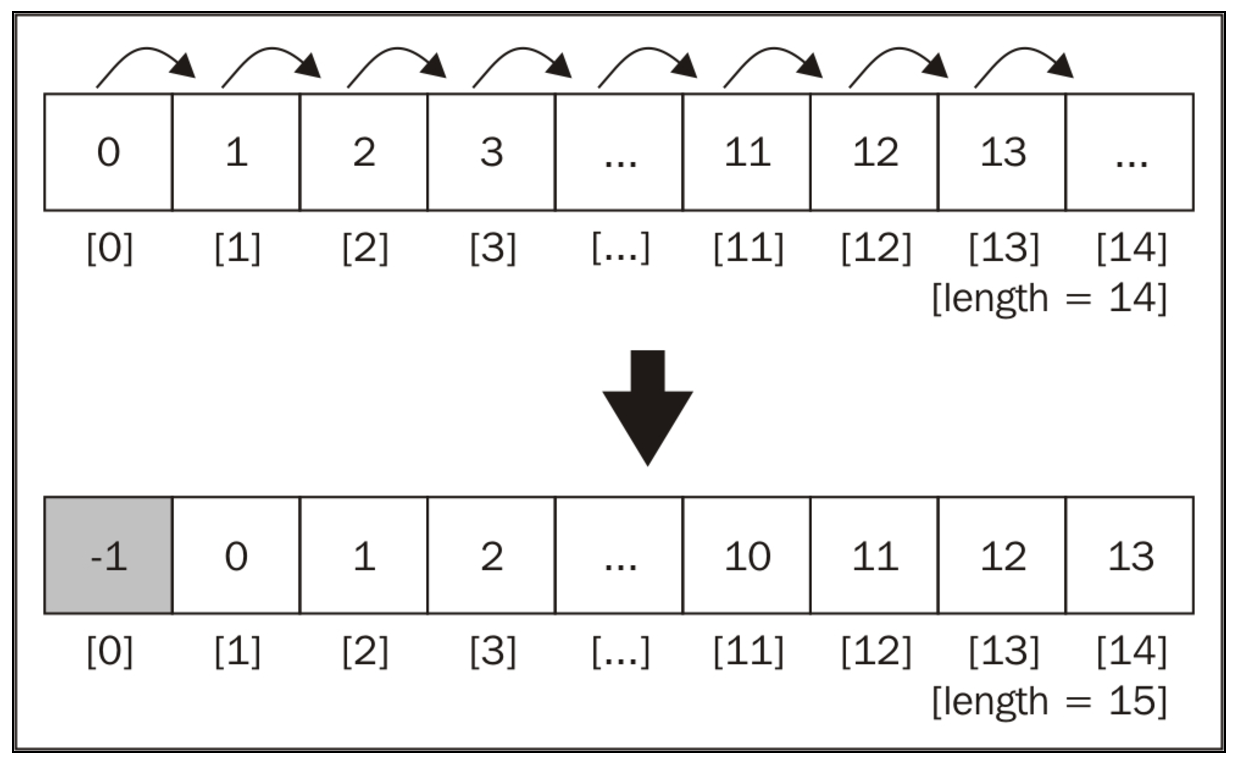
\includegraphics[scale=0.35]{pics/array_insert.png} \newline

	\item If you have an array of big object, and you need to sort it. You can build a array of pointer to point to each object in the array. When you sort the an array of big object,  you just move pointer instead, It is called \textbf{"indirect addressing"}, It can help you to avoid moving big chunk of data.  

	\item reverse array can be implemented by \textbf{swap + double pointers}, But reversing list need different algorithm, so in STL , \texttt{std::list} has its own reverse member function. 
\begin{lstlisting}[breaklines]
void reverseArray(int a [], int n){
	int i,j,temp;
	for(i=0,j=n-1;i<n/2;++i,--j){
		swap(a[i], a[j]);
	}
}
\end{lstlisting}
\begin{description}
	\item[line 3] remember: if \texttt{n} is size of array, \texttt{n/2} is the middle element(odd) or the first element in the second half(even). This pattern is very helpful for you to write reverse function. 
\end{description}

	\item Write a function rotate(ar[], d, n) that rotates arr[] of size n by d elements.
\begin{enumerate}
	\item single rotate method
\begin{lstlisting}[breaklines]
while(d-->0){ //d-- >0 is good trick
  int temp = Array[0];
  for (int i = 0; i < n-1; i++){
    Array[i] = Array[i + 1];
  }
  Array[n-1] = temp;
}
\end{lstlisting}

	\item Reverse method. That is a very efficient implementation.
\begin{lstlisting}[breaklines]
rotate(arr[], d, n)
  reverse(arr[], 1, d) ;
  reverse(arr[], d + 1, n);
  reverse(arr[], l, n);
\end{lstlisting}
\textbf{Idea: middle part reverse twice, so keep origin value}


	\item You can use rotate in insert sort method. also use in slide. Detail can be found in "Top 5 Beautiful C++ std Algorithms Examples"
\begin{lstlisting}[breaklines, basicstyle=\scriptsize]
for (auto i = start; i != end; ++i)
	std::rotate(std::upper_bound(start, i, *i), i, std::next(i));  
	//all stl algorithms deal with left open, right close space. 
	//i and std::next(i) is right close point                               

template <typename It> 
auto slide(It f, It l, randIter p) -> std::pair<It, It>{
  //  p < [f...l] < p, two possibles 
  if (p < f) return { p, std::rotate(p, f, l) };
  if (l < p) return { std::rotate(f, l, p), p };
  return { f, l };
}

ForwardIt rotate( ForwardIt first, ForwardIt n_first, ForwardIt last );
// rotate returns Iterator to the new location of the element pointed by first
\end{lstlisting}
\begin{description}
	\item[line 2:] rotate(a, b, c) is [a,b) and [b,c) scope. they are all left close, right open scope. In this way, you can understand why we need \texttt{std::next(i)} here.
\end{description}

	\item \textbf{reverse-->rotate--> insert order and slide}

\end{enumerate}

	\item We can also use partition to implement gather. \textbf{Partition return: Iterator to the first element of the second group.}

	\item Gather all eligible element around iterator p
\begin{lstlisting}[numbers=none]
template <typename BiIt, typename UnPred> 
auto gather(BiIt f, BiIt l, BiIt p, UnPred s) -> std::pair <BiIt, BiIt>{
	return { stable_partition(f, p, not1(s)), 
		stable_partition(p, l, s) };
}		
\end{lstlisting}


\end{itemize}

\subsection{Interview questions}
\subsubsection{common questions}
\begin{itemize}
	\item Two sum. 
\begin{enumerate}
\item Answer 1: Sort O(n*log(n))
\begin{lstlisting}[tabsize=3]
bool hasArrayTwoCandidates(int A[], int arr_size, int sum) { 
	int l, r; 
	sort(A, A + arr_size); 
	
	/* Now look for the two candidates in  
	the sorted array*/
	l = 0; 
	r = arr_size - 1; 
	while (l < r) { 
		if (A[l] + A[r] == sum) 
			return 1; 
		else if (A[l] + A[r] < sum) 
			l++; 
		else // A[i] + A[j] > sum 
			r--; 
	} 
	return 0; 
} 
\end{lstlisting}
\textbf{Idea: Don't need keep index information, so you can sort it. }

\item Answer 2: Hash O(n)
\end{enumerate}

\item Count triplets with sum smaller than a given value. 
\begin{lstlisting}[breaklines]
1) Sort the input array in increasing order. 
2) Initialize result as 0.
3) Run a loop from i = 0 to n-2.  An iteration of this loop finds all
   triplets with arr[i] as first element.
     a) Initialize other two elements as corner elements of subarray 
        arr[i+1..n-1], i.e., j = i+1 and k = n-1
     b) Move j and k toward each other until they meet, i.e., while (j < k)
            (i) if (arr[i] + arr[j] + arr[k] >= sum), then do k-- 

            // Else for current i and j, there can (k-j) possible third elements 
            // that satisfy the constraint.
            (ii) Else Do ans += (k - j) followed by j++ 
\end{lstlisting}
\textbf{Idea: Same Idea as previous question, Don't need keep index information, so you can sort it. }


	\item Given an array of positive integers. All numbers occur even number of times except one number which occurs odd number of times. Find the number in O(n) time and constant space.
Example: I/P = [1, 2, 3, 2, 3, 1, 3] and O/P = 3. The Best Solution is to do bitwise XOR of all the elements. XOR of all elements gives us odd occurring element. Please note that XOR of two elements is 0 if both elements are same and XOR of a number x with 0 is x.

\begin{lstlisting}[breaklines]
	result = result ^ a[i];
\end{lstlisting}
\textbf{Idea: Perform some calculation on all elements. }


	\item You are given a list of n-1 integers and these integers are in the range of 1 to n. There are no duplicates in list. One of the integers is missing in the list. Write an efficient code to find the missing integer.
\begin{lstlisting}[breaklines]
1) Get the sum of numbers 
       total = n*(n+1)/2
2  Subtract all the numbers from total and you will get the missing number.
\end{lstlisting}
\textbf{Idea: Perform some calculation on all elements. }

	\item Max product of the three numbers for a given array of size N. \textbf{Find the three largest numbers in the array (n1, n2, n3) and the two smallest numbers (m1, m2). The answer is either n1 x n2 x n3 or n1 x m1 x m2.}
\begin{lstlisting}[breaklines]
nth_element(...)
\end{lstlisting}
\textbf{Idea: Not sort, but nth max element based on heap}

	\item Given an unsorted array of non-negative integers, find a \textbf{continuous} subarray which adds to a given number.  Examples: Input: arr[] = {1, 4, 20, 3, 10, 5}, sum = 33; Ouptut: Sum found between indexes 2 and 4. 

\begin{lstlisting}[breaklines]
int arr[] = {1, 4, 20, 3, 10, 5};
int left = 0; int right = 0;
int sum = 0;
while(right< 6){
	sum+=arr[right];
	++right;
	
	while(sum>33){
		sum-=arr[left];
		++left;
		if (sum == 33){
			cout<<left<<" "<<right<<" "<<endl;
		}
	}	
}
\end{lstlisting}
\textbf{Idea: 1) You must keep index information, so you can't sort. }  \textbf{That is a typical sliding window problems. Keep head and trail two index. } Sliding window can be found in algorithm chapter. 

	\item Given an array \texttt{arr[]} of integers, find out the difference between any two elements such that larger element appears after the smaller number in arr[]. Examples: If array is [2, 3, 10, 6, 4, 8, 1] then returned value should be 8 (Diff between 10 and 2). If array is [ 7, 9, 5, 6, 3, 2 ] then returned value should be 2 (Diff between 7 and 9). That is also a one time stock buy sell problem.
\begin{lstlisting}[breaklines]
In this method, instead of taking difference of the picked element with every other element, we take the difference with the minimum element found so far. So we need to keep track of 2 things:
1) Maximum difference found so far (max\_diff).
2) Minimum number visited so far (min\_element).
\end{lstlisting}
\textbf{Keep position, but this problem can be divided by sub-problem. Such as, [ 7, 9, 5, 6, 3, 2 ] can be seen as [7,9] [5, 6] [3] [2]  Once current element is less than min\_element, begin a new sub-problem.}


	\item Inversion Count for an array indicates -- how far (or close) the array is from being sorted. If array is already sorted then inversion count is 0. If array is sorted in reverse order that inversion count is the maximum. Formally speaking, two elements a[i] and a[j] form an inversion if a[i] > a[j] and i < j. Example: The sequence 2, 4, 1, 3, 5 has three inversions (2, 1), (4, 1), (4, 3).

\begin{lstlisting}[breaklines]
int main(){
	vector<int> vi = {2, 4, 1, 3, 5};
	set<int> si;
	int sum = 0;
	for(auto i :vi){
		si.insert(i);
		cout<<i<<endl;
		auto it1 = si.upper_bound(i);
		if (it1 != si.end())
		cout<<"***"<<*it1<<endl;
		sum += distance(it1, si.end());
	}
	
	cout<<sum<<endl;
	return 0;
}
\end{lstlisting}
\begin{description}
	\item[Line 10:] \textbf{set also support iterator, it will output sorted element from beginning to end }
	\item[Line 12] \textbf{distance function, you have to input smaller iterator first. for set, if you input end, it will fall into dead loop}
\end{description}

\textbf{1) You need keep index(position) information. (No sort, no calculation).  2) you can't divid it to subj-problem. 3) You have to use auxiliary DS outside. such as set. which store how many element is greeter than current element.  }


	\item Convert array into Zig-Zag fashion ? The converted array should be in form a < b > c < d > e < f. 
\begin{lstlisting}[breaklines]
We can convert in O(n) time using an Efficient Approach. The idea is to use modified one pass of bubble sort. Maintain a flag for representing which order(i.e. < or >) currently we need. If the current two elements are not in that order then swap those elements otherwise not.
Let us see the main logic using three consecutive elements A, B, C. Suppose we are processing B and C currently and the current relation is '<'. But we have B > C. Since current relation is '<' previous relation must be '>' i.e., A must be greater than B. So, the relation is A > B and B > C. We can deduce A > C. So if we swap B and C then the relation is A > C and C < B. Finally we get the desired order A C B
\end{lstlisting}

\end{itemize}


\subsubsection{mono stack}
\begin{itemize}
	
	\item  Write a program to print all the LEADERS in the array. An element is leader if it is greater than all the elements to its right side. And the rightmost element is always a leader. For example int the array {16, 17, 4, 3, 5, 2}, leaders are 17, 5 and 2. 
	
\begin{lstlisting}[breaklines]
		Scan all the elements from right to left in array and keep track of maximum till now. When maximum changes it's value, print it.
		\textbf{Same idea just like previous}
\end{lstlisting}	
	
	\item Next Greater Element.  Given an array, print the Next Greater Element (NGE) for every element. The Next greater Element for an element x is the first greater element on the right side of x in array. Elements for which no greater element exist, consider next greater element as -1.
\begin{verbatim}
		Examples:
		a) For any array, rightmost element always has next greater element as -1.
		b) For an array which is sorted in decreasing order, all elements have next greater element as -1.
		c) For the input array [4, 5, 2, 25}, the next greater elements for each element are as follows.
	Element       NGE
	4      -->   5
	5      -->   25
	2      -->   25
	25     -->   -1
\end{verbatim}

\begin{lstlisting}[breaklines]
void printNGE(int arr[], int n){
	stack<int> s;
	
	/* push the first element to stack */
	s.push(arr[0]);

	// iterate for rest of the elements
	for (int i = 1; i < n; i++) {
		
		if (s.empty()) {
			s.push(arr[i]);
			continue;
		}
		
		/* if stack is not empty, then
		pop an element from stack.
		If the popped element is smaller
		than next, then
		a) print the pair
		b) keep popping while elements are
		smaller and stack is not empty */
		while (s.empty() == false && s.top() < arr[i]) {
			cout << s.top() 
			<< " --> " << arr[i] << endl;
			s.pop();
		}
		
		/* push next to stack so that we can find
		next greater for it */
		s.push(arr[i]);
	}
	
	/* After iterating over the loop, the remaining
	elements in stack do not have the next greater
	element, so print -1 for them */
	while (s.empty() == false) {
		cout << s.top() << " --> " << -1 << endl;
		s.pop();
	}
}
\end{lstlisting}	
%单调栈的一个主要的理念就是针对不同的问题,把一些不满足条件的元素不压入栈(丢弃掉,因为他们对答案没有意义。)

\end{itemize}	

\subsubsection{mono queue}
\begin{itemize}
	\item Given an array and an integer K, find the maximum for each and every contiguous subarray of size k.
\begin{enumerate}
	\item The first brute force, O(n*k). 
	\item The second, use balance Search Tree(std::set), O(n*log(k)). 
	\item the third, use queue O(n)
\begin{lstlisting}[breaklines]
    std::deque<int> Qi(k);

	/* Process first k (or first window) elements of array */
	int i;
	for (i = 0; i < k; ++i) {
		
		// For every element, the previous
		// smaller elements are useless so
		// remove them from Qi
		while ((!Qi.empty()) && arr[i] >= arr[Qi.back()])
		
		// Remove from rear
		Qi.pop_back();
		
		// Add new element at rear of queue
		Qi.push_back(i);
	}

	// Process rest of the elements, 
	// i.e., from arr[k] to arr[n-1]
	for (; i < n; ++i) {
		
		// The element at the front of 
		// the queue is the largest element of
		// previous window, so print it
		cout << arr[Qi.front()] << " ";
		
		// Remove the elements which 
		// are out of this window
		while ((!Qi.empty()) && Qi.front() <= i - k)
		
		// Remove from front of queue
		Qi.pop_front(); 
		
		// Remove all elements 
		// smaller than the currently
		// being added element (remove 
		// useless elements)
		while ((!Qi.empty()) && arr[i] >= arr[Qi.back()])
		Qi.pop_back();
		
		// Add current element at the rear of Qi
		Qi.push_back(i);
	}

	// Print the maximum element 
	// of last window
	cout << arr[Qi.front()];	
\end{lstlisting}	
	
	\item The conclusion. It looks like two sum problem. there are three different levels time complexity. 
\end{enumerate}

	
\end{itemize}


\subsubsection{hints for array questions.}

\begin{enumerate}
	\item Clue1: Get max and min value, based on heap, init a heap need O(n), when you get the second largest or third largest one, you only need O(log(n)). It's better than sort O(n*log(n) ). 
	
	\item Clue2: Sort, it will lose the index information. 
	
	\item Clue3: For continuous subarray, keep head and trail two index. two indexes can be used in reverse, and two sums. 
	
	\item Clue4: Calculate, such as sum and bit operator XOR. 
	
	\item Clue5: Use other auxiliary DS, such as, map, set or hash\_map.  They can be used as count and sort. 
\end{enumerate}

\begin{itemize}
	\item A few common use pattern.  \newline
	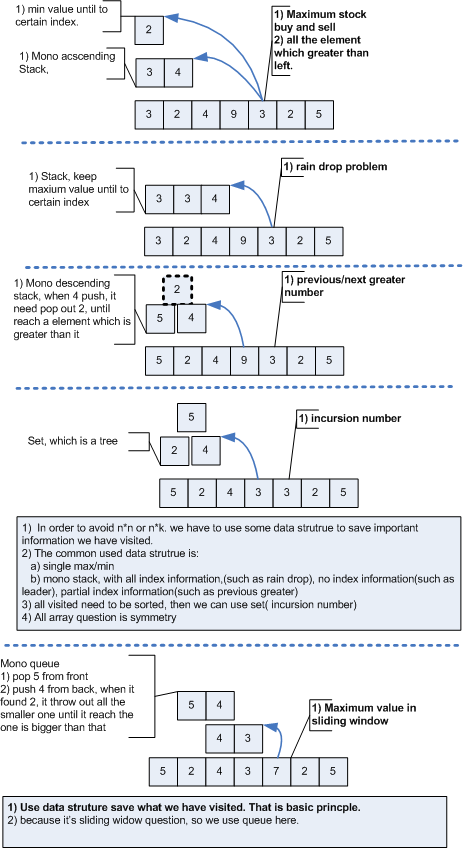
\includegraphics[scale=0.65]{pics/array.png} \newline
	
\end{itemize}




\section{Linked list}
\subsection{Basic}
\begin{itemize}
\item list in STL is bidirectional list(double-linked), in C++11, you can use \texttt{forward\_list} as single-linked list. 


\item  Declaration of Linked list. 
\begin{lstlisting}[frame=single, language=c++]
//C 
struct node{ 
int a; 
 struct node* link
} ;

//C++
Template <class T>
Class ChainNode{
   friend Chain<T>;
   T data
  ChainNode<T> *link;
}

template<class T>
class Chain{
......
ChainNode<T> *head;
}
\end{lstlisting}
\begin{description}
	\item[C++] I think that \texttt{std::list} is implemented in this way.
\end{description}

\end{itemize}


\subsection{Operations}
\begin{itemize}
\item insert, \textbf{get an index to previous pointer}
\begin{lstlisting}[frame=single, language=c++, mathescape=true]
//Consider if it's the first element. 
Insert(int k, const T &x)
chainNode<T> *i = new chainNode<T> (x);

//leftside is pointer pointed direction
//rightside is node, but in list, all nodes only can be accessed by a pointer.
//insert after p node 
i->link = p->link;
p->link = i;
// i is inserted element, p is position.  
//You can remember i=p p=i  and fore three links.
\end{lstlisting}

\item insert, before p node, what should I do?  \textbf{Just swap two node, then deal with next node. Don't touch next node in one atomic action. That is rule. }
\begin{lstlisting}[frame=single, language=c++, mathescape=true]
1)create temp auto node, new a i node.
 
while(p->link) 
2) copy value from p to temp node
3) copy value i to p.
4) copy temp value to i value
p = p->link.  
\end{lstlisting}

\item delete the node after a given node.
\begin{lstlisting}[frame=single, language=c++]
Delete(int k, const T&x)
d = p->link;
p->link = d->link ;
delete d;
//d=p p=d and last three links
\end{lstlisting}

\item delete the given node. That is a typical question. you need to remember it. 
\begin{lstlisting}[frame=single, language=c++]
void deleteNode(Node* node_ptr){
	// If the node to be deleted is the 
	// last node of linked list
	if (node_ptr->next == NULL)
	{
		free(node_ptr);
		// this will simply make the node_ptr NULL.
		return;
	}
	
	// if node to be deleted is the first or 
	// any node in between the linked list.
	Node* temp = node_ptr->next;
	node_ptr->data = temp->data;
	node_ptr->next = temp->next;
	free(temp);
}
\end{lstlisting}
\begin{description}
	\item[Source code] Psychically, still delete the next node, logically, we use next value to overwrite current node value, so we simulate "delete" in this way. 
\end{description}

\item Indirect addressing combines array and list. You should store pointer in array, and each pointer refer to random storage object. A typical usage is char* [] each item in array is char*(string), when you sort the strings, you just move pointers. It will save a lot of move time.  

\item three different operations:
\begin{enumerate}
	\item normal single link list: insert and delete given a node, always insert after the given node, or erase the next node of the given node. 
	
	\item normal single link list: If you want to insert before or delete the given node, You still need to do it physically, but copy value to simulate the "insert" and "delete". 
	
	\item double link list, such as \texttt{std::list}, insert value before the given node, and delete the given node. 
\end{enumerate}

\item In STL, list has its own sort(merge sort), unique, reverse, remove operation. because it's different with generic algorithms. 

\item How to rotate a List?

\begin{lstlisting}[frame=single, language=c++]
list<int> li = {1, 2, 3, 4, 5};
auto i = begin(li);
//rotate(i, next(i, 3), end(li) );
li.splice(i, li,next(i, 3), end(li) );
\end{lstlisting}
\begin{description}
	\item[Line 3:] You can use generic algorithm, but must use next.time complexity is O(n).
	\item[Line 4:] You can also use splice, The complexity is O(1).
\end{description}

\end{itemize} 

\subsection{Application}
\subsubsection{Bucket sort}

\begin{itemize}
\item For each item, the value range is limited, and is integer. For example, sort all students score. (0<=score<=100). 

\item Basic step:  Here, Link list is best option to implement a bucket. Because Nobody will now how many elements will be put into the each bucket. 
\begin{enumerate}
\item Set up an array of initially empty "buckets".
\item Scatter: Go over the original array, putting each object in its bucket. 
\item Sort each non-empty bucket.(Optional )
\item Gather: Visit the buckets in order and put all elements back into the original array.
\end{enumerate}

\end{itemize}

\subsubsection{Radix sort}

\begin{itemize}
\item r is radix, $x\%r, (x\%r^{2})/r, (x\%r^{3})/r^{2}$  get each digit from least significant digit (LSD) radix sorts to most significant digit. 

\begin{lstlisting}[frame=single, language=c++]
int i ;
int k;
while(i%10){
	k = i%10;
	i = i/10;
}
\end{lstlisting}

\begin{enumerate}
\item according to r, prepare two arrays buckets A, B. 
\item Sort according to one position and put them into A array buckets. 
\item loop through A array buckets, and get next position digit. and then according to its value put into B array buckets.
\item swap A,B two array, then goto step 2.
\end{enumerate}

	\item Difference between radix sort and quick sort. Quicksort/Introsort is more flexible:Quicksort and Introsort work well with all kinds of data. All you need for sorting is the possibility to compare items. This is trivial with numbers but you can sort other data as well. Radix sort on the other hand just sorts things by their binary representation. It never compares items against each other. Radix sort needs more memory. All radix sort implementations that I've seen use a secondary buffer to store partial sorting results. This increases the memory requirements of the sorting algorithm. That may not be a problem if you only sort a couple of kilobytes, but if you go into the gigabyte range it makes a huge difference. If I remember right a in place radix-sort algorithm exist on paper though.

\end{itemize}


\subsubsection{Other interview questions}
\begin{itemize}
	\item print the middle. 
\begin{lstlisting}[breaklines]
/* Function to get the middle of the linked list*/
void printMiddle(struct Node *head) 
{ 
	struct Node *slow_ptr = head; 
	struct Node *fast_ptr = head; 
	
	if (head!=NULL) {
		 
		while (fast_ptr != NULL && fast_ptr->next != NULL) {  //this statement is very important.
			fast_ptr = fast_ptr->next->next; 
			slow_ptr = slow_ptr->next; 
		} 
		printf("The middle element is [%d]\n\n", slow_ptr->data); 
	} 
} 
\end{lstlisting}
\begin{description}
	\item[source code] when exit while, even node, fast\_ptr will be NULL, odd node, fast\_ptr->next will be null.
	\item[source code] \textbf{Just like n/2, odd number will be in the middle, even number will be the first element in the second half.}
\end{description}
	
	\item How to reverse a list \textbf{ There are two points: 1)while(p),  2) inside loop, do p = p->next, and necessary action( print out value and change pointer direction...)}
\newline

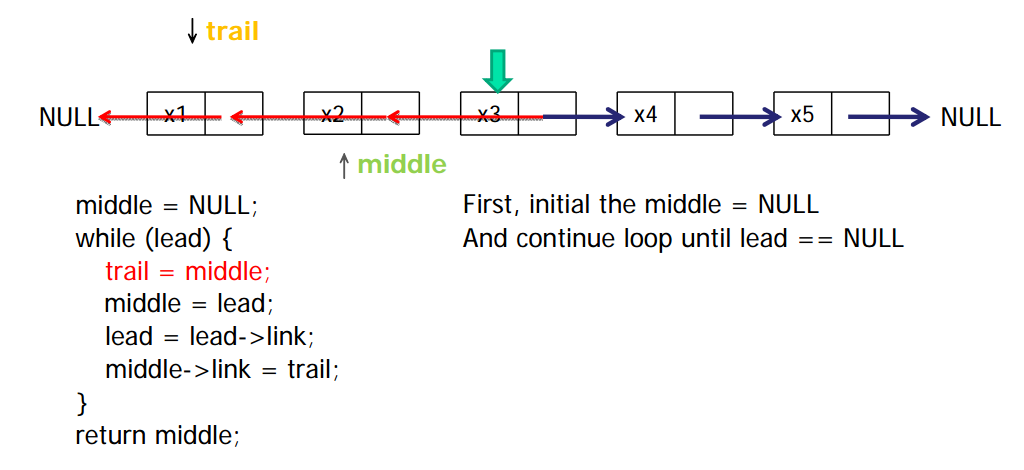
\includegraphics[scale=0.65]{pics/reverse.png} \newline

\begin{lstlisting}[breaklines]
node* lead; 
node *middle, *tail;
middle = nullptr;
tail = head;
while(tail){
	lead = middle;
	middle = tail;
	tail = tail->next;
	middle->next = lead;
}

head = middle;
\end{lstlisting}
\begin{description}
	\item[line] end condition
	\item[line] end-input condition
	\item[line] begin condition
	\item[line] begin-input condition
\end{description}

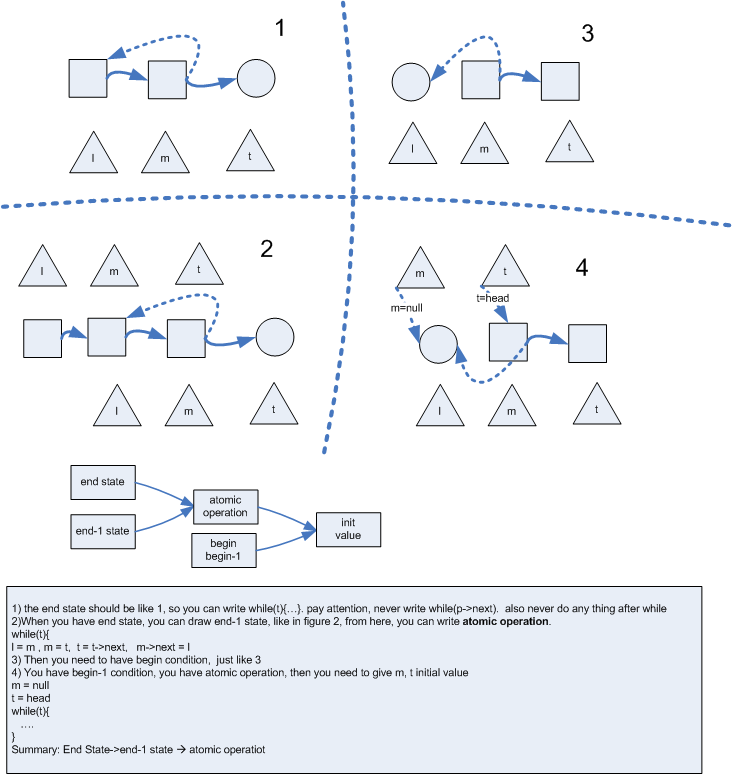
\includegraphics[scale=0.60]{pics/link.png} \newline


	\item Given a singly linked list, determine if its a palindrome. This method takes O(n) time and O(1) extra space.
\begin{enumerate}
	\item Get the middle of the linked list.
	\item Reverse the second half of the linked list.
	\item Check if the first half and second half are identical.
	\item \textbf{Idea: 1) find the middle 2)reverse}. If it's odd number,  you need to move the middle pointer to next position.
\end{enumerate}


	\item Swap nodes in a linked list without swapping data. 
\begin{lstlisting}[breaklines]
The idea it to first search x and y in given linked list. If any of them is not present, then return. While searching for x and y, keep track of current and previous pointers.
\end{lstlisting}


	\item Merge sort is often preferred for sorting a linked list. The slow random-access performance of a linked list makes some other algorithms (such as quicksort) perform poorly, and others (such as heapsort) completely impossible. MergeSort(headRef)
\begin{verbatim}
1) If head is NULL or there is only one element in the Linked List 
    then return.
2) Else divide the linked list into two halves.  
      FrontBackSplit(head, &a, &b); /* a and b are two halves */
3) Sort the two halves a and b.
      MergeSort(a);
      MergeSort(b);
4) Merge the sorted a and b (using SortedMerge() discussed here) 
   and update the head pointer using headRef.
     *headRef = SortedMerge(a, b);
\end{verbatim}
\textbf{Idea: 1) No random access 2) recursive}

\begin{lstlisting}[frame=single, language=c++] 
/* sorts the linked list by changing next pointers (not data) */
void MergeSort(struct node** headRef)
{
  struct node* head = *headRef;
  struct node* a, b;
 
  /* Base case -- length 0 or 1 */
  if ((head == NULL) || (head->next == NULL)){
    return;
  }

  /* Split head into 'a' and 'b' sublists */
  FrontBackSplit(head, &a, &b); 
 
  /* Recursively sort the sublists */
  MergeSort(&a);
  MergeSort(&b);
 
  /* answer = merge the two sorted lists together */
  *headRef = SortedMerge(a, b);
}

\end{lstlisting}

 \begin{lstlisting}[frame=single, language=c++] 
/* See http://geeksforgeeks.org/?p=3622 for details of this 
   function */
struct node* SortedMerge(struct node* a, struct node* b)
{
  struct node* result = NULL;
 
  /* Base cases */
  if (a == NULL)
     return(b);
  else if (b==NULL)
     return(a);
 
  /* Pick either a or b, and recur */
  if (a->data <= b->data){
     result = a;
     result->next = SortedMerge(a->next, b);
  }
  else{
     result = b;
     result->next = SortedMerge(a, b->next);
  }
  return(result);
}
 \end{lstlisting}
\begin{description}
	\item[Source code:] \textbf{Idea: recursive}
\end{description}
 
 \begin{lstlisting}[frame=single, language=c++] 
/* UTILITY FUNCTIONS */
/* Split the nodes of the given list into front and back halves,
     and return the two lists using the reference parameters.
     If the length is odd, the extra node should go in the front list.
     Uses the fast/slow pointer strategy.  */
void FrontBackSplit(struct node* source,
          struct node** frontRef, struct node** backRef)
{
  struct node* fast;
  struct node* slow;
  if (source==NULL || source->next==NULL)
  {
    /* length < 2 cases */
    *frontRef = source;
    *backRef = NULL;
  }
  else
  {
    slow = source;
    fast = source->next;
 
    /* Advance 'fast' two nodes, and advance 'slow' one node */
    while (fast != NULL)
    {
      fast = fast->next;
      if (fast != NULL)
      {
        slow = slow->next;
        fast = fast->next;
      }
    }
 
    /* 'slow' is before the midpoint in the list, so split it in two
      at that point. */
    *frontRef = source;
    *backRef = slow->next;
    slow->next = NULL;
  }
}

\end{lstlisting}

	\item Merge Two sorted lists.
\begin{lstlisting}[frame=single, language=c++]
/* Takes two lists sorted in increasing order, and splices
   their nodes together to make one big sorted list which
   is returned.  */
struct node* SortedMerge(struct node* a, struct node* b){
    /* a dummy first node to hang the result on */
    struct node dummy;
    /* tail points to the last result node  */
    struct node* tail = &dummy;

    /* so tail->next is the place to add new nodes
      to the result. */
    dummy.next = NULL;
    while (1){
        if (a == NULL)        {
            /* if either list runs out, use the
               other list */
            tail->next = b;
            break;
        }
        else if (b == NULL){
            tail->next = a;
            break;
        }
        if (a->data <= b->data)
            MoveNode(&(tail->next), &a);
        else
            MoveNode(&(tail->next), &b);
 
        tail = tail->next;
    }
    return(dummy.next);
    //dummy code will be destoried. 
}
 \end{lstlisting}


	\item prints the given Linked List in reverse manner. 
\begin{lstlisting}[frame=single, language=c++]
void fun1(struct node* head){
  if(head == NULL)
    return;
  
  fun1(head->next);
  printf("%d  ", head->data);
}
\end{lstlisting}
\textbf{Idea: recursive}


	\item Write a program function to detect loop in a linked list
\begin{lstlisting}[breaklines]
This is the fastest method. Traverse linked list using two pointers.  Move one pointer by one and other pointer by two.  If these pointers meet at some node then there is a loop.  If pointers do not meet then linked list doesn't have loop.
\end{lstlisting}
\textbf{a circle has at last three nodes, so fast pointer each time step 2, So it will always go around inside the circle}

	\item Conclusion:
\begin{enumerate}
\item Just like tree, link-list problems can be resolved by recursive. 
\item Most of time, In single link list, you need to keep previous pointer. 
\end{enumerate}

\begin{tabular}{|c|c|c|}
\hline 
 & array & list \\ 
\hline 
insert erase & O(n) & O(1) \\ 
\hline 
sort & quicksort & mergesort  \\ 
\hline 
reverse & swap element & just manipulate pointer  \\ 
\hline 
rotate & easy pointer manipulate & swap element  \\ 
\hline 
merge &  &  \\ 
\hline 
other  &  &  \\ 
\hline 

\end{tabular} 

\begin{enumerate}
\item in STL,  For assign, insert, erase and constructor, vector support two version, one is single element, other is range.  When we deal wih range input, we prefer to use range version. 
\item std::list and std::vector has different big O for insert and erase.
\item std::list has its own sort member function, but std::vector doesn't have. you can use std::sort algorithme. 
\item std::list has its own reverse,  std::vector doesn't have, just use std::reverse algorithm
\item list and vector don't have their own rotate function.
\item list has its own merge, vector use std::merge algorithm.

\end{enumerate}

\end{itemize}

\section{Matrix}
\begin{itemize}
\item You can use two dimensions array to act as a matrix, square matrix, diagonal matrix, lower triangular, symmetric. 
\item Some special square matrix
\begin{enumerate}
\item Diagonal  $i\neq j, M(i,j) = 0$ Can use one dimension array to describe it. 
\item Low triangular $i<j, M(i,j) = 0$ We can use one dimension array to implement lower triangular because it will save many spaces.  Index can be calculated by $i*(i-1)/2+j-1$. and save it into a one dimension array. 
\item Symmetric. Just like Low triangular, can be descriped by one dimenstion array. 
\end{enumerate}
\end{itemize}

\subsubsection{sparse matrix}
\begin{itemize}
\item Sparse matrix can implemented by on dimension array or  linked list. 
\begin{lstlisting}[frame=single, language=c++]
template<typename T>
class term{
int row, int col;
T value;
}

Term<T> *sparseMatrix;
\end{lstlisting}

\item Sparse matrix in linked list.  \textbf{Three level definition}
\begin{lstlisting}[frame=single, language=c++]
template<typenameT>
class CNode{
int col;
T value;
};



template<typename T>
class HeadNode{
int row, 
Chain< CNode<T> > colFirst
};
  
template<typename T>
class Matrix{
  Chain< HeadNode<T> > Frist
} 
\end{lstlisting}


	\item You can build a matrix class. use m(2,3) to access a element. And support +, - * . You also can define index begin from 1. It will more reasonable for you when you use a matrix. 
\begin{lstlisting}[frame=single, language=c++]
template<typename T>
class Matrix{
T& operator()(int row, int col){
..}
}
\end{lstlisting} 

\end{itemize}

\subsection{interview questions}
\begin{itemize}
	
	\item Two matrix multiply. 
	\begin{lstlisting}[]
		int inner_product(int row, int col, int num, const vector<vector<int>> &v1, 
		const vector<vector<int>> &v2){
			int sum = 0;
			for (int i =0 ;i<num ;i++){
				sum += v1[row][i]*v2[i][col];
			}
			return sum;
		}
		
		vector<vector<int> > m1 = {{1,2,3}, {4, 5, 6}}; //list initialization
		vector<vector<int> >m2 = { {1,2}, {3,4}, {5,6}};
		int m1_row = m1.size();
		int m1_col = m1[0].size();
		int m2_row = m2.size();
		int m2_col = m2[0].size();
		vector<vector<int> > result = {{0,0}, {0,0}};
		for(int i = 0;i<m1_row;i++){
			for(int j= 0;j<m2_col;j++){
				int element = inner_product(i, j,3, m1, m2); //call function here.
				result[i][j] = element;
			}
		}	
	\end{lstlisting}
	
	\begin{description}	
		\item[line 1] In this questions, inner\_product is key point to resolve this problem. First, get atomic operation and change it into a function. Then, design this function parameter and in the end, design outside environment to call this automic function. This is very an important strategy. 
	\end{description}
	
	
	\item sprial print a matrix
	\begin{lstlisting}[numbers=none]
		int
		print_out (int rb, int re, int cb, int ce, bool isrow, bool positive,
		const vector < vector < int >>&v)
		{
			if (isrow){
				if (positive){
					for (int i = cb; i <= ce; i++){
						cout << v[rb][i]<<',';
					}
				}
				else{
					for (int i = ce; i >= cb; i--){
						cout << v[re][i]<<',';
					}
				}
			}
			else
			{
				if (positive){
					for (int i = rb; i <= re; i++){
						cout << v[i][ce]<<',';
					}
				}
				else{
					for (int i = re; i >= rb; i--){
						cout << v[i][cb]<<',';
					}
				}
			}
		}
		
		int main ()
		{
			vector < vector < int >>m1 = { {1, 2, 3}, {4, 5, 6}, {7, 8, 9} };
			int row = m1.size()-1;
			int col = m1[0].size()-1;
			
			int rb = 0, re = row, cb = 0, ce = col;
			int isrow = 1;
			int positive = 1;
			while (rb <= re && cb <= ce){
				
				if (isrow == 1 && positive == 1)
				{
					print_out (rb, re, cb, ce, isrow, positive,m1);
					rb++;
					isrow = 0;
					positive =1;
				}
				if (isrow == 0 && positive == 1)
				{
					print_out (rb, re, cb, ce, isrow, positive,m1);
					ce--;
					isrow = 1;
					positive = 0;
				}
				if (isrow == 1 && positive == 0)
				{
					print_out (rb, re, cb, ce, isrow, positive,m1);
					re--;
					isrow = 0;
					positive = 0;
				}
				if (isrow == 0 && positive == 0)
				{
					print_out (rb, re, cb, ce, isrow, positive,m1);
					cb++;
					isrow = 1;
					positive = 1;
				}
			}
			return 0;
		}	
		
	\end{lstlisting}		
	
	\begin{description}
		\item[line ] \textbf{In this questions, print\_out is key. }
		\item[line ] \textbf{Get atomic operation, print\_out, design the interface of this key function. after it, design the context which use this key function: print\_out. In this context, usually involve a loop and change boundary parameter.}
		
		\item[line ] rb, re, cb, ce very good clue, once you found these four parameters, then this question becomes easier. another two useful flag is isrow and positive. 
	\end{description}
\end{itemize}

 
\section{Stack}
\begin{itemize}
	\item In C++ STL , \texttt{std::stack} is container adaptor, specifically designed to operate in a LIFO context. 

	\item Stack is last-in first-out, and queue is frist-in and first-out
\end{itemize}


\subsection{Application of Stack}
\begin{itemize}
		
\item The most famous application about stack is \textbf{Recursive}. \textbf{The most famous applications based on stack is:  Maze(depth first). Hanoi tower. brace Match, recursive.}  


\item MinStack, all operation are constant time.
\begin{lstlisting}[frame=single, language=c++, basicstyle=\scriptsize]
class MinStack {
	public:
	void push(int val) {
		if (stack.empty()) {
			stack.push_back({val, val});
		} else {
			stack.push_back({val, min(stack.back().second, val)});
		}
	}
	
	void pop() {
		stack.pop_back();
	}
	
	int top() {
		return stack.back().first;
	}
	
	int getMin() {
		return stack.back().second;
	}
	
	private:
	// first = val, second = min as of that insert
	vector<pair<int, int> > stack;
};
\end{lstlisting}

	\item some typical two stacks examples. One is expressions evaluation. we can build two stacks, one is for operands and the other for operators. When the operators precedence is higher than the stack top element, push the operators into the stack, otherwise, pop the operator and get two operatands from operands stacks, get the result and push back to the operands stack.  
	\begin{center}
			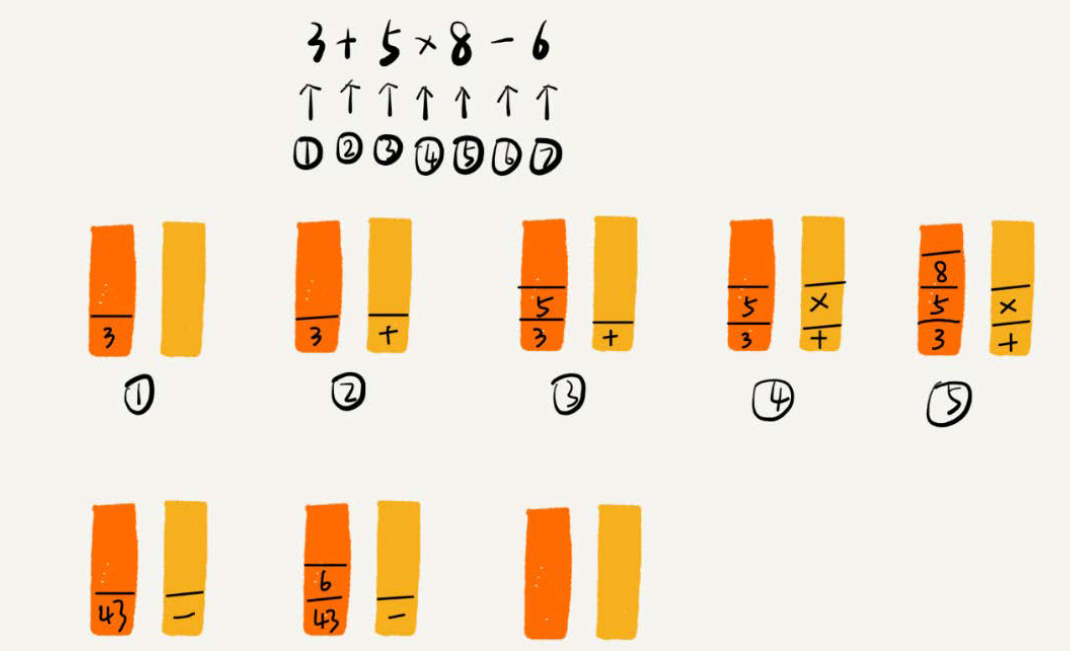
\includegraphics[scale=0.45]{pics/stacks_two.png} 
	\end{center}

	\item two stacks trick can also be used in browers back and forward function. Another typical two stack usage are use two stacks to implement queue
	
	\begin{center}
		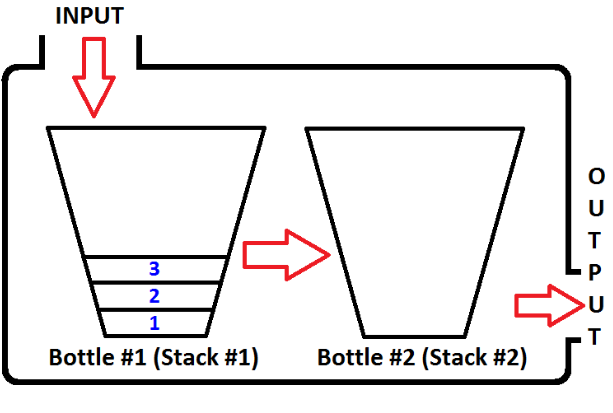
\includegraphics[scale=0.3]{pics/sq1.png} 
	\end{center}
	\begin{center}
		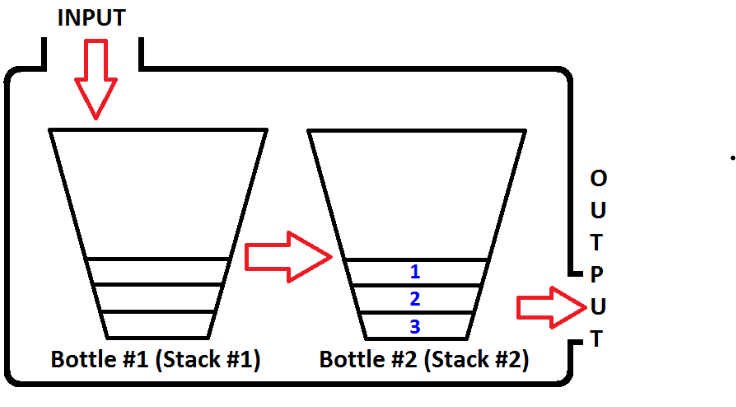
\includegraphics[scale=0.3]{pics/sq2.png} 
	\end{center}
	

	

\end{itemize}

\subsubsection{Offline Equivalence class}
\begin{itemize}
	\item offline equivalence class, known n and R, get all Equivalence class. 
	
	\item n = 9, r = 11 and relation pairs are:
	(1,5), (1,6),(3,7),(1,5), (4,8),(5,2)
	(6,5), (4,9),(9,7),(7,8), (3,4),(6,2)
	
	\item Two phases to determine equivalence class
	
	\item One word, \textbf{from relation pairs build a graphs(adjacency list), Then use stack to perform DFS search, use equivalence class record if we have visited.}
	
	
	
	Phase 1: Equivalence pairs (i, j) are read in and adjacency (linked) list of each object is built.
	Phase 2: Trace (output) the equivalence class containing object i with stack (depth-first search). Next find another object not yet output, and repeat.
	
\begin{lstlisting}[frame=single, language=c++, basicstyle=\scriptsize]
	for (int i = 1; i <= n; i++)  // output equivalence classes
	if  (!out[i]) { // start of a new class
		out[i] = true;
		unprocessedList.push(new Integer(i)) ;
		while (!unprocessedList.empty()) { 
			// get rest of class from unprocessedList
			int j = ((Integer) unprocessedList.pop()).intValue();
			while  (!list[j].empty()) { 
				// elements on list[j] are in the same class
				int q = ((Integer) list[j].pop()).intValue();
				if (!out[q]) { // q not yet output
					System.out.print(q + " ");
					out[q] = true;
					unprocessedList.push(new Integer(q));  }
			} //end of while
		}  //end of while 
	} //end of if
\end{lstlisting}		

	
	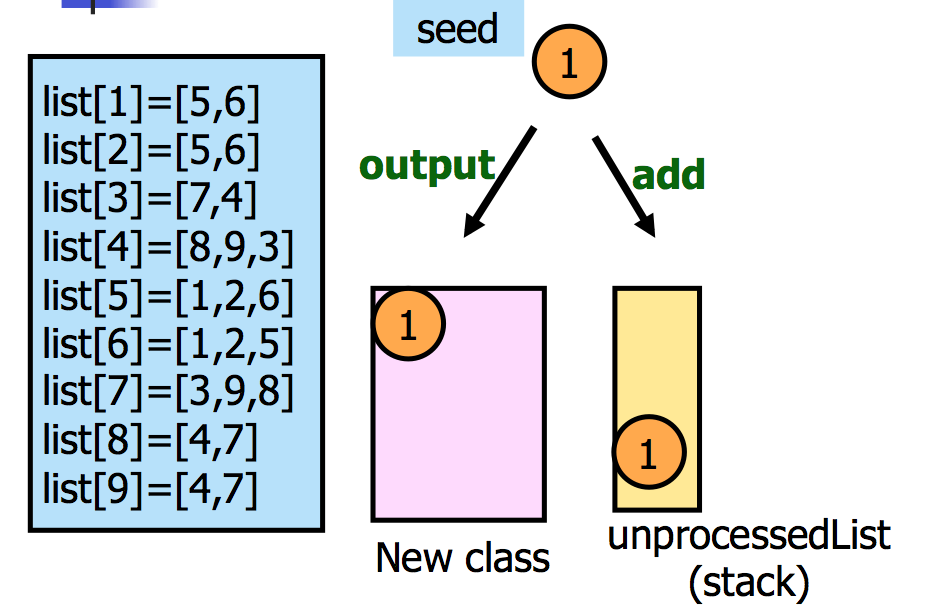
\includegraphics[scale=0.35]{pics/offline_1.png} \newline
	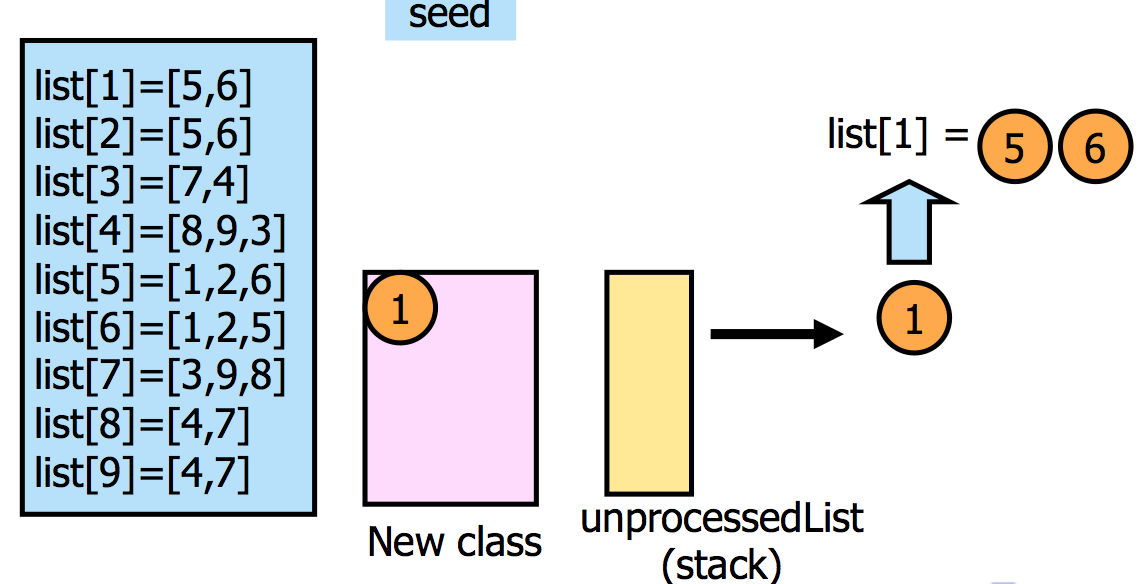
\includegraphics[scale=0.35]{pics/offline_2.png}  \newline
	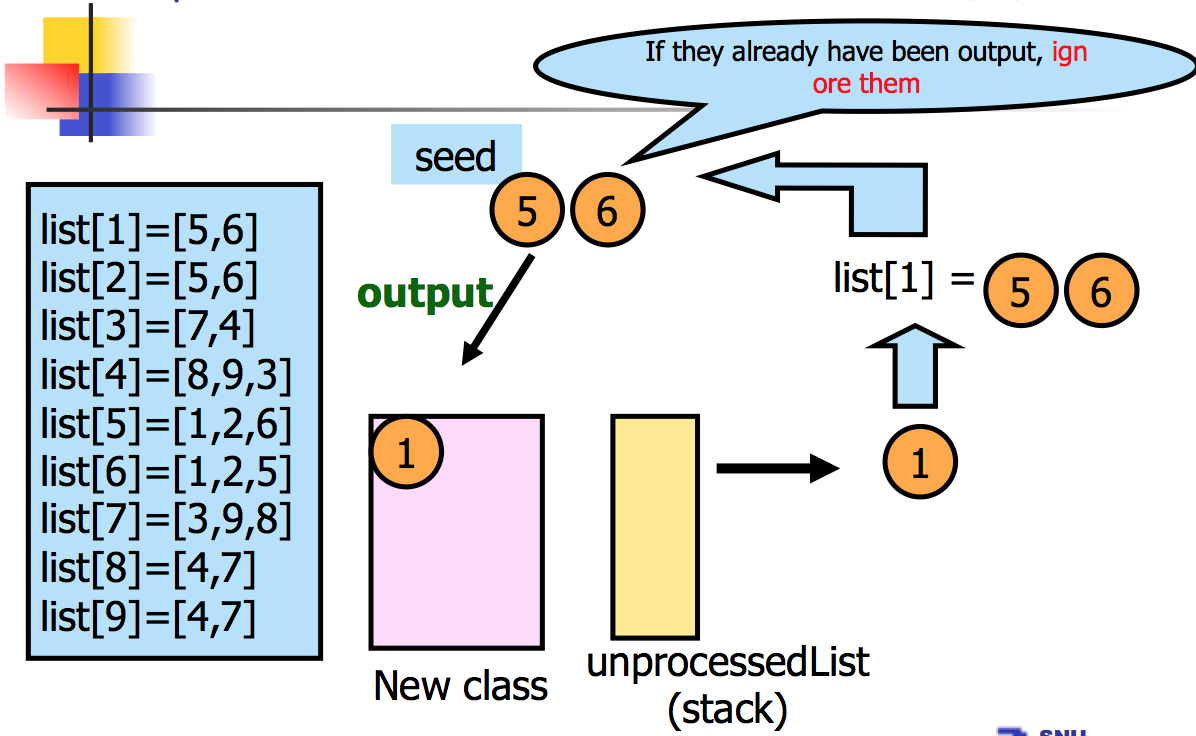
\includegraphics[scale=0.35]{pics/offline_3.png} \newline
	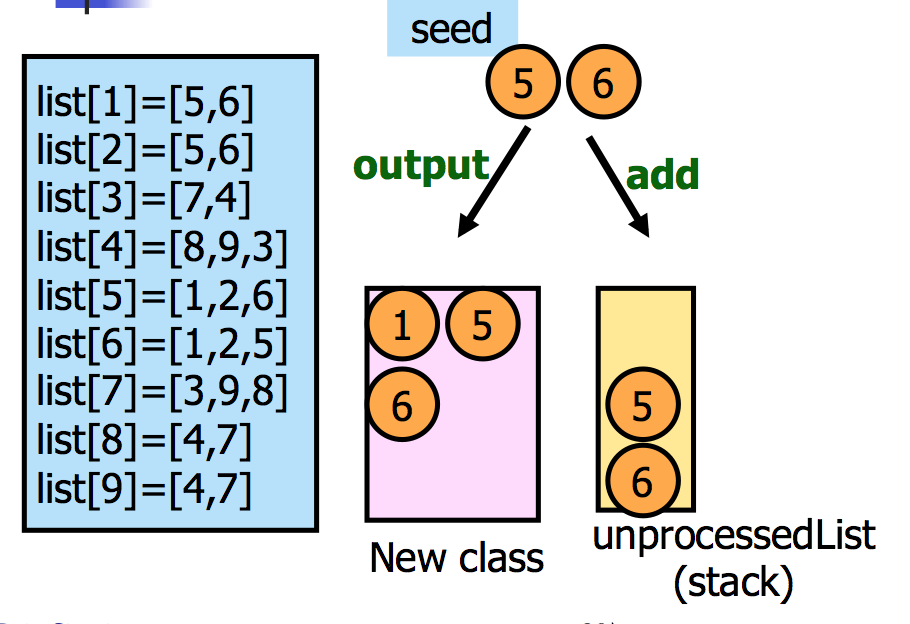
\includegraphics[scale=0.35]{pics/offline_4.png} \newline
	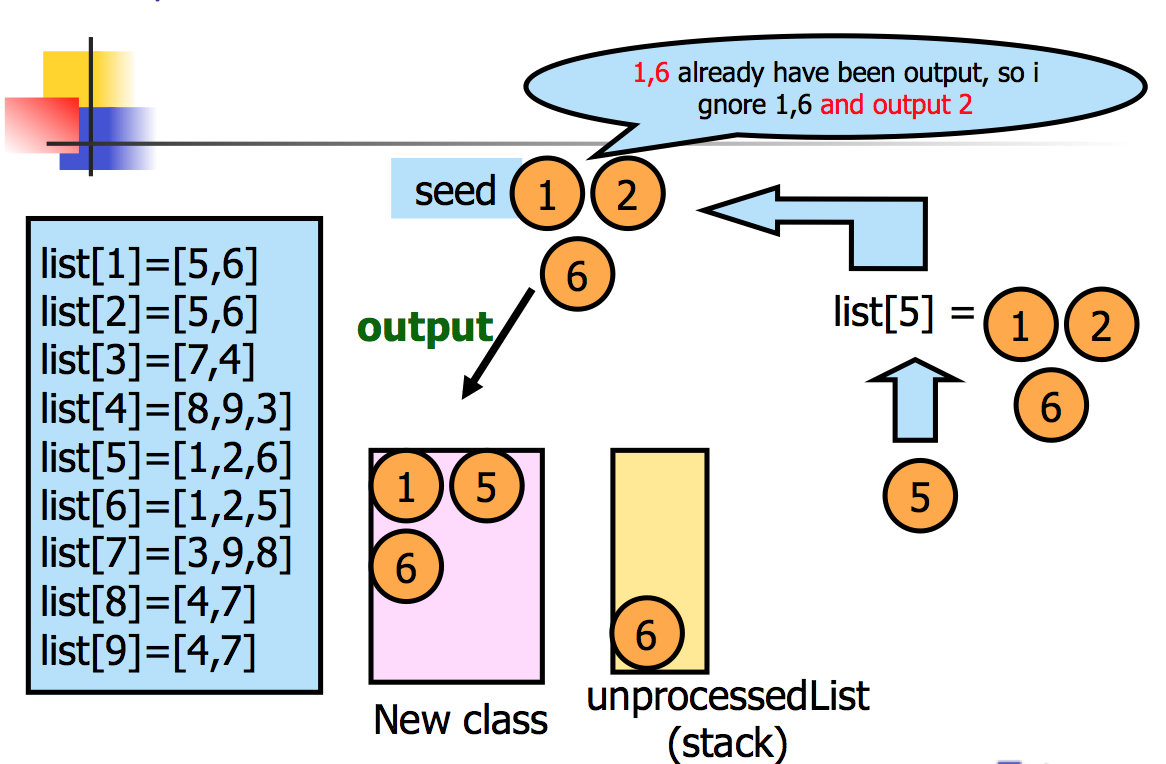
\includegraphics[scale=0.35]{pics/offline_5.png} \newline
	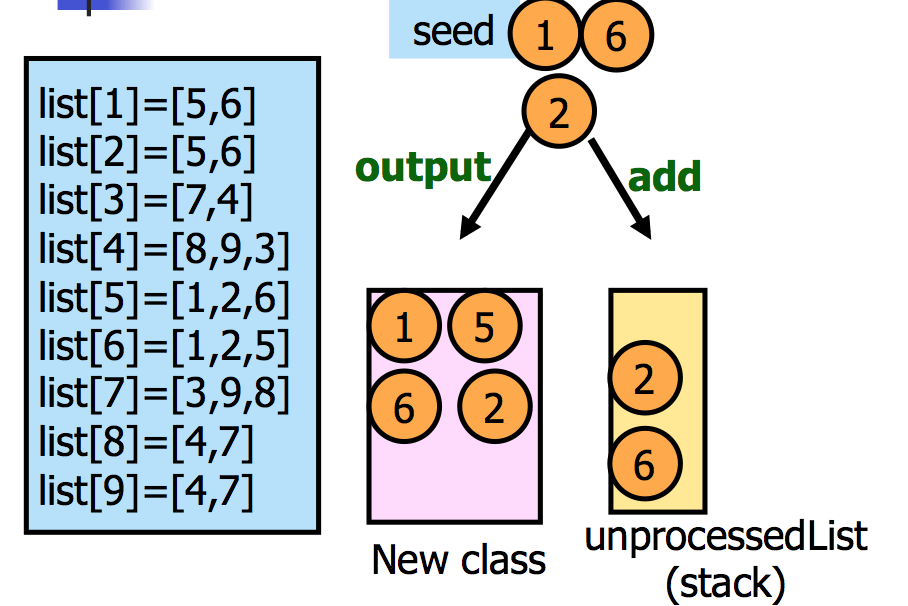
\includegraphics[scale=0.35]{pics/offline_6.png} \newline

\end{itemize}


\section{Queue}
\begin{itemize}
\item In STL, Queue has front() and back() interface. 

\end{itemize}


\subsection{Circule Queue}
\begin{itemize}
	
\item You can use three different way to implement queue, array, linked list and circular array.
	
\item circular array representation of a queue
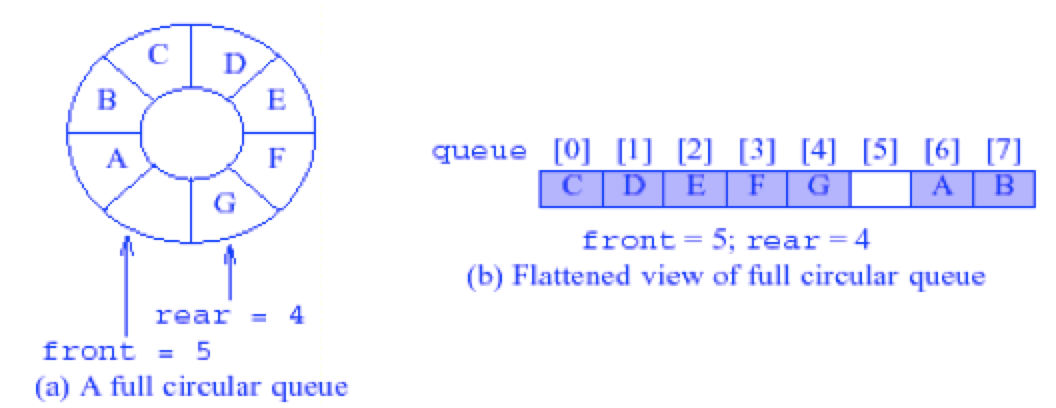
\includegraphics[scale=0.35]{pics/cd.png} \newline
\begin{enumerate}
\item Initial condition : front = rear = 0
\item Empty queue:     front == rear
\item Full: (rear+1)\%length == front
\item \textbf{front point to an empty cell. So at mast it can save length-1 elements. } Otherwise, we can't distinguish empty and full.

\item push only increase rear, so if (rear+1)\%length == front, means rear catch up front, it means full. 
\begin{lstlisting}[frame=single, language=c++]
void push(T t){
	if ((rear+1)%length == front){
		throw "full" exception
	}
	rear = (rear+1)%length;
	array[rear] = t;
}	
\end{lstlisting}

\item pop only increase front, so if front == rear, means front catch up rear, it means empty.
\begin{lstlisting}[frame=single, language=c++]
T pop(){
	if (front == rear){
		throw "empty" exption
	}
	front = (front+1)%length;
	return array[front];
}
\end{lstlisting}

\end{enumerate}

\end{itemize}


\subsection{Application of queue}
\begin{itemize}
\item  BFS maze 
\begin{lstlisting}[frame=single, language=c++]
here=root of T;
here is end?
enqueue(Q,v);

while(!empty(Q)){
    dequeue(Q, here);
    if(here is end)
    for (each next position of here){
        if(next position is not end){
             mark next position
             enqueue(Q, next position);
        }
    }
}
\end{lstlisting}

\item For BFS, path is not save in stack. So you need a new kind of data type. 
\begin{lstlisting}[frame=single, language=c++]
struct position {
        int x;
        int y;
        struct position* parent;
}
\end{lstlisting}
\item Just like DFS, before you add a position to queue, mark it first. 

\end{itemize}



\section{Heap}
\subsection{Basic}
\begin{itemize}
	
\item Why heap sort has nlog(n)?

\verb|https://stackoverflow.com/questions/54078858/why-is-the-time-complexity-of-heap-sort-onlogn|
	
\item Max(min) tree is each node is greater or equal to its children node.

\item two basic operations: sink and swim.

\item Heap is \textbf{1)complete 2) binary 3)Max(min) tree.} Because Heap is complete binary tree. We can use an array to store it. 

\item insert is easier than you think, When you insert, put it on the end position, then exchange with parent.  
\begin{lstlisting}[frame=single, language=c++, mathescape=true]
insert(x){
	int c = ++currentSize;
	while(c!=1 && x>heap[c/2]){ //get its parent node and compare
		heap[c] = heap[c/2];  //move down parent
		$\Hilight{20}$// move parent  down because it smaller
		c/=2;  //move up a level 
	}  
	heap[c] = x;  //the right position of insert. 
	//at this time heap[c] has been moved away by previous 
	//statement heap[c] = heap[c/2] 
}
$\Hilight{20}$ //c is used to control level,  c/=2 move up level
$\Hilight{20}$ //heap[c/2] get its parent	
\end{lstlisting}

\item \textbf{Heap just support delete Max(Min) value.} When delete, delete the first element, then put the end position element to the first position, then exchange it with either left child or right child. 
\begin{lstlisting}[frame=single, language=c++, mathescape=true]
T y = heap[CurrentSize--];
int i = 1, ci = 2;
//because ci will increase to get bigger one from two children.
//so I have to use another i to keep current level
while(ci<=CurrentSize){
	if(heap[ci]<heap[ci+1]) ci++; // get the bigger child
	
	if(y>=heap[ci]{
		heap[i] = y;   // i always empty for a new value. 
		break; 
	}
	$\Hilight{10}$ //i is current node
	$\Hilight{10}$ //ci  is i biggest child node
	heap[i] = heap[ci]; //move up child, insert is "move down parent"
	i = ci;  //move to next level
	ci *=2;
}	
\end{lstlisting}



\item Initialize a Heap: \textbf{For an array, from the middle point, loop backward until reach to beginning( 0 index)}. the time complexity is O(n). 

\begin{lstlisting}[frame=single, language=c++]
void heapify(int arr[], int n, int i)
{
	int largest = i; // Initialize largest as root
	int l = 2 * i + 1; // left = 2*i + 1
	int r = 2 * i + 2; // right = 2*i + 2
	
	// If left child is larger than root
	if (l < n && arr[l] > arr[largest])
	largest = l;
	
	// If right child is larger than largest so far
	if (r < n && arr[r] > arr[largest])
	largest = r;
	
	// If largest is not root
	if (largest != i) {
		swap(arr[i], arr[largest]);
		
		// Recursively heapify the affected sub-tree
		heapify(arr, n, largest);
	}
}

// Function to build a Max-Heap from the given array
void buildHeap(int arr[], int n){
	// Index of last non-leaf node
	int startIdx = (n / 2) - 1;
	
	// Perform reverse level order traversal
	// from last non-leaf node and heapify
	// each node
	for (int i = startIdx; i >= 0; i--) {
		heapify(arr, n, i);
	}
}
\end{lstlisting}

\item Heap just guarantees that elements on higher levels are greater (for max-heap) or smaller (for min-heap) than elements on lower levels, whereas BST guarantees order (from "left" to "right"). If you want sorted elements, go with BST.

\item In STL, heap is called priority\_queue

\begin{lstlisting}[frame=single, language=c++, mathescape=true, basicstyle=\scriptsize]
//default compare function is less<T>
std::priority_queue<int, std::vector<int>, std::greater<int> > q2;
for(int n : {1,8,5,6,3,4,0,9,7,2})
	q2.push(n);
    // 0, 1, 2 ,3 ,4, 5...
\end{lstlisting}


\item STL support a basic heap operation

\begin{lstlisting}[frame=single, language=c++, mathescape=true]
	vector<int> vi = {2, 4, 1, 3, 5,6,7};
	cout<<"ddd"<<distance(end(vi),begin(vi))<<endl;
	make_heap(begin(vi),end(vi)); // inpace modify
	
	//after you pop_heap, you need to use v.pop_back()
	//to make begin(vi), end(vi) is still heap. 
	v.pop_heap(begin(vi),end(vi));
	v.pop_back();
	
	//if you want to use push_heap, you have to 
	//call push_back first. 
	v.push_back(10);
	v.push_heap(v.begin(vi) ,end(vi));
	
	//still inpace modify
	sort_heap(v.begin(vi) ,end(vi));
\end{lstlisting}
\begin{description}
	\item[source code] \textbf{push\_back and push\_heap must appear together. }. At the same time. \textbf{pop\_heap and pop\_back must appear together. }
\end{description}

%head 只支持三种操作,初始化,插入和删掉最大(小)值。  插入在最后位置,然后不断和父节点交换以便满足条件。 删掉是先删掉最值,然后把最后一个位置的值转移到root,然后在分别和左右子节点比较以便决定和那个子节点交换一边满足条件。编程过程中一个重要一点是对于父节点和子节点的关系如下:
\begin{lstlisting}
Root is at index 0 in array.
Left child of i-th node is at (2*i + 1)th index.
Right child of i-th node is at (2*i + 2)th index.
Parent of i-th node is at (i-1)/2 index.
\end{lstlisting}

\end{itemize}

\subsection{application}
\begin{itemize}
\item \textbf{Huffman tree use external nodes to represent a character, It assure no prefix is repeated }
\item You can use minHeap to build huffman tree. in the minHeap, each element is child tree, and then pop twice, combine two child trees. then insert it back to minHeap. Until there is only one element in the Heap. 

\item top k item in data steam. \textbf{use K minimum heap} 

\item median number in data steam. \textbf{use one minimum heap and one maximum heap, and keep these two heaps has at least 1 number difference size.} 
\end{itemize}

\section{Tree}
\subsection{Basic knowledge}
\subsubsection{Basic conception}
\begin{itemize}
\item List has a first node, every tree has a root node. Root node is a key component when you deal with most of tree problems.  

\item Pre-order, In-order and Post-order are based on middle node. \textbf{and they are all dfs algorithm.}

\item complete, full, perfect tree are different. Full Binary can be skewed shape. 
\begin{enumerate}
	\item Full Binary Tree: A Binary Tree is full if every node has 0 or 2 children. 
	
	
	\item Complete Binary Tree: A Binary Tree is complete Binary Tree if all levels are completely filled except possibly the last level and the last level has all keys as left as possible. (complete tree is heap, so complete tree is very important conception.)
	
	\item Perfect Binary Tree: A Binary tree is Perfect Binary Tree in which all internal nodes have two children and all leaves are at same level.
\end{enumerate}
	
\begin{verbatim}
     18  //full binary tree
   /    \   
  15      20    
 /  \       
40   50   
	/  \
	30  50
	
         18   //complete (heap is complete tree)
    /         \  
   15           30  
  /  \         /  \
 40    50     100   40
/  \   /
8   7  9 
	
	
      18     //perfect 
   /       \  
  15        30  
 /  \       /  \
40    50   100   40
\end{verbatim}


\item Heap is CBT(complete binary tree), not perfect binary tree. 

\item Balance search tree includes AVL and RB tree, in order to keep it balance, you need to rotate child tree. 

\item Tournament Tree: Tournament tree is a complete binary tree with some properties. Remove and  Replay of Tournament tree gives you "sorting". 

\item Binary Search Tree: BST is a binary tree with some properties (not necessarily CBT). In-order traversal of BST gives you "sorting" Can be skewed and unbalanced, so we need Balanced Tree.

\end{itemize}

\subsubsection{Other property of tree}
\begin{itemize}
	\item level, horizontal, and diagonal traversal.
	
	\item horizontal distance is distance between root node.  when you want to have bottom view or top view, you can use it.  detail can be found here: \newline
	\verb|https://www.techiedelight.com/print-bottom-view-of-binary-tree/|
	
\begin{lstlisting}[frame=single, language=c++]
map<int, pair<int, int>> map;
printBottom(root, 0, 0, map);
//---------------------------------------	
void printBottom(Node* node, int dist, int level, auto &map)
{
	// base case: empty tree
	if (node == nullptr) {
		return;
	}
	
	// if the current level is more than or equal to the maximum level seen so far
	// for the same horizontal distance or horizontal distance is seen for
	// the first time, update the map
	
	if (level >= map[dist].second)
	{
		// update value and level for the current distance
		map[dist] = { node->key, level };
	}
	
	// recur for the left subtree by decreasing horizontal distance and
	// increasing level by 1
	printBottom(node->left, dist - 1, level + 1, map);
	
	// recur for the right subtree by increasing both level and
	// horizontal distance by 1
	printBottom(node->right, dist + 1, level + 1, map);
}
\end{lstlisting}
\begin{description}
	\item[line 1] distance and level should be stack type value.
	\item[line 1] map is reference can shared by all recursive functions. And this is very important data structure in this question. 
\end{description}

	\item diagonal  \verb|https://www.techiedelight.com/find-diagonal-sum-given-binary-tree/|
\begin{lstlisting}[frame=single, language=c++]
// Recursive function to perform preorder traversal on the tree and
// fill the map with the diagonal sum of elements
 unordered_map<int, int> map;
void diagonalSum(Node* root, int diagonal, auto &map)
{
	// base case: empty tree
	if (root == nullptr) {
		return;
	}
	
	// update the current diagonal with the node's value
	map[diagonal] += root->data;
	
	// recur for the left subtree by increasing diagonal by 1
	diagonalSum(root->left, diagonal + 1, map);
	
	// recur for the right subtree with the same diagonal
	diagonalSum(root->right, diagonal, map);
}
	
\end{lstlisting}
\begin{description}
	\item[line 1] diagonal is just add 1 when you go to the left tree. Don't change when you go right tree. 
	\item[line 1] when you use sum of the whole tree, you must pass a reference type value. 
\end{description}	

\end{itemize}

 
\subsection{Search Tree}
\begin{itemize}
\item Search tree is the key in each node must be \textbf{greater than all keys stored in the left sub-tree, and smaller than all keys in the right sub-tree.} 

\item Difference between BST and hash
\begin{enumerate}
\item So Hash Table seems to beating BST in all common operations. When should we prefer BST over Hash Tables? what are advantages? Following are some important points in favor of BSTs.

\item We can get all keys in sorted order by just doing Inorder Traversal of BST. This is not a natural operation in Hash Tables and requires extra efforts.

\item Doing order statistics, finding closest lower and greater elements, doing range queries are easy to do with BSTs. Like sorting, these operations are not a natural operation with Hash Tables.

\item BSTs are easy to implement compared to hashing, we can easily implement our own customized BST. To implement Hashing, we generally rely on libraries provided by programming languages.

\item With BSTs, all operations are guaranteed to work in O(Log(n) ) time. But with Hashing, O(1) is average time and some particular operations may be costly, especially when table resizing happens.
\end{enumerate}

\item ascending or descending order of BST. Pay attention here, they are all in order traversal.
\begin{lstlisting}[frame=single, language=c++]
void ascending(BST* root){
    if(root == NULL) return;
    ascending(root->left);
    std::cout<<root->data<<" ";
    ascending(root->right);
}
 
void descending(BST* root){
    if(root == NULL) return;
    descending(root->right);
    std::cout<<root->data<<" ";
    descending(root->left);
}
\end{lstlisting}

\end{itemize}


\subsection{Tree and recursion} 
\subsubsection{Base case}


\begin{itemize}

\item \textbf{Nearly all the tree problems can be resolved by recursive}.

\item \textbf{Only focus on the current root logic.} For example, kth element problem, or lowest common ancester problem.

\item The basic patter is below: 
\begin{lstlisting}[frame=single, language=c++]
TreeFun(root*...){
	BaseCase;
	TreeFun(root->Left...);
	TreeFun(root->right...);
	Join
}
\end{lstlisting}

\begin{enumerate}
	\item 95\% Base Case is very simple.\textbf{Forgetting to check if the root is null. It's an important base case. In nearly all interview questions, the first statement inside recursive should be check root, then return nullptr, return 0 or return nothing.}
\begin{lstlisting}
	if(root == nullptr){
		return ...
	}
\end{lstlisting}
	
	\item The easier part is recursive all with left child and right child. At this time, you should design the recursive interface according to specific question. For example, If it is required from you to write a function that returns a value (e.g. the number of nodes in a binary tree), you have to make sure that the function actually "returns". One of the common mistakes is just writing the recursive call without writing the word "return" before it.
	
	\item The most difficult part is \textbf{Join}, You should write some logic here according to specific problem.
	
	\item For example, for the height of tree, we need to get max value of the left and right tree and increment it. 
\begin{lstlisting}[frame=single, language=c++]
private int height(Node t){
	if(t == null)  {  //1) base case
		return -1;   //5) return value 
	}
	else
	{
		int height = 1 + max( height(t.left), height(t.right) );
		//5) put left and right recursive into assignment
		return height;
	}
}		
\end{lstlisting}	
	
\end{enumerate}

\end{itemize}


\subsubsection{span child tree}
\begin{itemize}
	\item Determine whether the given binary tree nodes are cousins of each other. Two nodes of a binary tree are cousins if they have the same depth, but have different parents.   \textbf{traversal all, use global variable to store the good result when you traversal all. } 
\begin{lstlisting}[frame=single, language=c++]
// Perform inorder traversal on a given binary tree and update `x` and `y`
void inorder(Node* root, Node* parent, int level, NodeInfo &x, NodeInfo &y)
{
	// base case: tree is empty
	if (root == nullptr) {
		return;
	}
	
	// traverse left subtree
	inorder(root->left, root, level + 1, x, y);
	
	// if the first element is found, save its level and parent node
	if (root->key == x.key)
	{
		x.level = level;
		x.parent = parent;
	}
	
	// if the second element is found, save its level and parent node
	if (root->key == y.key)
	{
		y.level = level;
		y.parent = parent;
	}
	
	// traverse right subtree
	inorder(root->right, root, level + 1, x, y);
}
\end{lstlisting}
\begin{description}
	\item[label] use two global valure as reference, then search the whole tree. 
\end{description}

\end{itemize}

\subsubsection{order}

\begin{itemize}
	

\item Next big question is pre-order, in-order or post-order. \textbf{90\% we use post-order.} But it also depends on practical requirement.


\begin{enumerate}
	\item inorder: two applications
	Find k’th smallest and k’th largest element in a BST:
\begin{lstlisting}[frame=single, language=c++]
int kthSmallest(Node* root, int *i, int k){
	// base case
	if (root == nullptr) {
		return INT_MAX;
	}
	// Left
	int left = kthSmallest(root->left, i, k);
	
	// Join
	if (left != INT_MAX) {
		return left;
	}
	
	// if the current element is k'th smallest, return its value
	if (++*i == k) {
		return root->data;
	}
	
	// right
	return kthSmallest(root->right, i, k);
}
\end{lstlisting}
\begin{description}
	\item[1] Only In order tranversal give ascending order, we have to use here.
	
	\item[1] for example, kth element, you only think that the element in left tree, then return it, current root, then return it.  if it's in right tree, then recursive call with root->right.
	
	\item[1] return INT\_MAX can be thought as a flag. if you want to look for a integer, you can use INT\_MAX to denote a flag.
	
	\item[1] i should be shared by all recursive call, so we use pointer or reference here. 
\end{description}

\item print an expression tree
\begin{lstlisting}[frame=single, language=c++]
     *
   /  \
  +    c
 / \
a   b
	
void inorder(Node* root)
{
	if (root == nullptr) {
		return;
	}
	
	// if the current token is an operator, print open parenthesis
	if (isOperator(root->data)) {
		cout << "(";
	}
	
	inorder(root->left);
	cout << root->data;
	inorder(root->right);
	
	// if the current token is an operator, print close parenthesis
	if (isOperator(root->data)) {
		cout << ")";
	}
}
\end{lstlisting}

\item preorder:
Print left view of a binary tree
\begin{lstlisting}[frame=single, language=c++]
// Recursive function to print the left view of a given binary tree
void leftView(Node* root, int level, int &last_level)
{
	// base case: empty tree
	if (root == nullptr) {
		return;
	}
	
	// if the current node is the first node of the current level
	if (last_level < level)
	{
		// print the node's data
		cout << root->key << " ";
		
		// update the last level to the current level
		last_level = level;
	}
	
	// recur for the left and right subtree by increasing the level by 1
	leftView(root->left, level + 1, last_level);
	leftView(root->right, level + 1, last_level);
}
\end{lstlisting}

\item postorder: 
Find maximum sum root to leaf path in a binary tree
\begin{lstlisting}[frame=single, language=c++]
// Function to calculate the maximum root-to-leaf sum in a binary tree
int getRootToLeafSum(Node* root){
	// base case: tree is empty
	if (root == nullptr) {
		return 0;
	}
	
	// calculate the maximum node-to-leaf sum for the left child
	int left = getRootToLeafSum(root->left);
	
	// calculate the maximum node-to-leaf sum for the right child
	int right = getRootToLeafSum(root->right);
	
	// consider the maximum sum child
	return (left > right? left : right) + root->data;
}	
\end{lstlisting}

\item combined:
find LCA
\begin{lstlisting}[frame=single, language=c++]
bool findLCA(Node* root, Node* &lca, Node* x, Node* y)
{
	// base case 1: return false if the tree is empty
	if (root == nullptr) {
		return false;
	}
	
	// base case 2: return true if either `x` or `y` is found
	if (root == x || root == y){  // 
		// set lca to the current node
		lca = root;
		return true;
	}
	
	// recursively check if `x` or `y` exists in the left subtree
	bool left = findLCA(root->left, lca, x, y);
	
	// recursively check if `x` or `y` exists in the right subtree
	bool right = findLCA(root->right, lca, x, y);
	
	// if `x` is found in one subtree and `y` is found in the other subtree,
	// update lca to the current node
	if (left && right) {
		lca = root;
	}
	
	// return true if `x` or `y` is found in either left or right subtree
	return left || right;
}
\end{lstlisting}
\begin{description}
	\item[] \textbf{Only focus on the current root logic}. If left anf right , then return root. otherwise just return left or right.  so simple!!
\end{description}


\item level order:
\begin{lstlisting}[frame=single, language=c++]
// Function to print spiral order traversal of a given binary tree
void spiralOrderTraversal(Node* root)
{
	if (root == nullptr) {
		return;
	}
	
	// create an empty double-ended queue and enqueue the root node
	list<Node*> deque;        // or use deque
	deque.push_front(root);
	
	// `flag` is used to differentiate between odd or even level
	bool flag = false;
	
	// loop till deque is empty
	while (!deque.empty())
	{
		// calculate the total number of nodes at the current level
		int nodeCount = deque.size();
		
		// print left to right
		if (flag)
		{
			// process each node of the current level and enqueue their
			// non-empty left and right child to deque
			while (nodeCount)
			{
				// pop from the front if `flag` is true
				Node* curr = deque.front();
				deque.pop_front();
				
				cout << curr->key << " ";
				
				// it is important to push the left child into the back,
				// followed by the right child
				
				if (curr->left != nullptr) {
					deque.push_back(curr->left);
				}
				
				if (curr->right != nullptr) {
					deque.push_back(curr->right);
				}
				
				nodeCount--;
			}
		}
		
		// print right to left
		else {
			// process each node of the current level and enqueue their
			// non-empty right and left child
			while (nodeCount)
			{
				// it is important to pop from the back
				Node* curr = deque.back();
				deque.pop_back();
				
				cout << curr->key << " ";    // print front node
				
				// it is important to push the right child at the front,
				// followed by the left child
				
				if (curr->right != nullptr) {
					deque.push_front(curr->right);
				}
				
				if (curr->left != nullptr) {
					deque.push_front(curr->left);
				}
				
				nodeCount--;
			}
		}
		
		// flip the flag for the next level
		flag = !flag;
		cout << endl;
	}
}
\end{lstlisting}
\begin{description}
	\item[] use BFS, so use queue, but we also need spiral, so have to use deque which support pop\_front and pop\_back.
	
	\item[] In order to print each level, use below source code pattern.
\begin{lstlisting}[frame=single, language=c++]
while (!deque.empty()){
	// calculate the total number of nodes at the current level
	int nodeCount = deque.size();	
	while(nodeCound){
		nodeCount--;
\end{lstlisting}	

\end{description}


\item conclusion: 
\begin{enumerate}
	\item Most of time, traversal order can be decided by the question itself very quickly.
	\item \textbf{any time when you find Maximum or ancestor, this is a strong indication which we can use postorder.}
	\item You can combined use preorder and postorder together. such as ??
\end{enumerate}

\end{enumerate}

\end{itemize}

\subsubsection{Interface}

\begin{itemize}
	\item Next questions is interface design. (all auxiliary parameter)
Find k’th smallest and k’th largest element in a BST:  \texttt{int *i} is shared variable among all recursive. which record how many nodes we have visited so far. return value is just your question answer. that is very easy to understand. 
	

\item \textbf{If you change inside function, sometimes, you need to change it back when you return.}
\begin{lstlisting}[frame=single, language=c++]
// Recursive function to find paths from the root node to every leaf node
void printRootToleafPaths(Node* node, vector<int> &path)
{
	// base case
	if (node == nullptr) {
		return;
	}
	
	// include the current node to the path
	path.push_back(node->data);
	
	// if a leaf node is found, print the path
	if (isLeaf(node))
	{
		for (int data: path) {
			cout << data << " ";
		}
		cout << endl;
	}
	
	// recur for the left and right subtree
	printRootToleafPaths(node->left, path);
	printRootToleafPaths(node->right, path);
	
	// backtrack: remove the current node after the left, and right subtree are done
	path.pop_back();
}	
\end{lstlisting}

\item Another simple is use local stack variable. If you don't use reference, you don't need to pop\_back.
\begin{lstlisting}[frame=single, language=c++]
// Recursive function to find paths from the root node to every leaf node
void printRootToleafPaths(Node* node, vector<int> path)
{
	// base case
	if (node == nullptr) {
		return;
	}
	
	path.push_back(node->data);
	
	// if a leaf node is found, print the path
	if (isLeaf(node))		{
		for (int data: path) {
			cout << data << " ";
		}
		cout << endl;
	}
	
	// recur for the left and right subtree
	printRootToleafPaths(node->left, path);
	printRootToleafPaths(node->right, path);
	
}		
\end{lstlisting}


\item Information flow:
\begin{enumerate}
	\item  return value from child to parent, (only return one value, so need some calculation inside from both left and right children)
	\item pass from parent to child, parameter to remember auto value(level) , 
	\item shared between children and parent. and pass a pointer parameter(max\_level) to remember static, which all recursive 
\end{enumerate}
	
\end{itemize}




\subsubsection{traps}
\begin{itemize}
	\item \textbf{Checking if one or both children are null. You SHOULD NOT do that.} When you do the recursive call and pass the root.left() or the root.right() as the parameter, the recursive function will call itself and treating the passed child as the new root. So, you don't need to explicitly check if the children are null.
	
\item The above statement should be understood correctly. If current operation 
\begin{lstlisting}[frame=single, language=c++]
int countLeaves(Node* t){
	if(t == null) 
	return 0;
	
	if(isLeaf(t))  {
		return 1;
	}
	else
		return countLeaves(t.left) +countLeaves( t.right);
}	
	
\end{lstlisting}	
	
	\item \textbf{Accessing the children values. You SHOULD NOT do that.} The same as the previous point. The child passed to the recursive call is treated as the new root. So, you don't need to explicitly access the children values. Just make sure you do that for the root.
	
	
\end{itemize}



\subsubsection{two trees}

\begin{itemize}
	\item recursive can be used to deal with two trees at the same time. 
\begin{lstlisting}[frame=single, language=c++]
	int identicalTrees(struct node* a, struct node* b){
		/*1. both empty */
		if (a==NULL && b==NULL)
		return true;
		
		/* 2. both non-empty -> compare them */
		if (a!=NULL && b!=NULL)    {
			return(
			a->data == b->data &&
			identicalTrees(a->left, b->left) &&
			identicalTrees(a->right, b->right)
			);
		} 
		
		/* 3. one empty, one not -> false */
		return false;
	} 
\end{lstlisting}	

\item some problems can be changed to two tree problems. such as if mirror. 

\begin{lstlisting}[frame=single, language=c++]
// Function to check if subtree rooted at `X` and `Y` mirror each other
bool isSymmetric(Node* X, Node* Y)
{
	// base case: if both trees are empty
	if (X == nullptr && Y == nullptr) {
		return true;
	}
	
	// return true if
	// 1. Both trees are non-empty, and
	// 2. The left subtree is the mirror of the right subtree, and
	// 3. The right subtree is the mirror of the left subtree
	return (X != nullptr && Y != nullptr) &&
	isSymmetric(X->left, Y->right) &&
	isSymmetric(X->right, Y->left);
}
\end{lstlisting}


\item fill any nodes next pointer:
\begin{lstlisting}[frame=single, language=c++]
Node connect(Node root) {
	if (root == null) return null;
	connectTwoNode(root.left, root.right);
	return root;
}

void connectTwoNode(Node node1, Node node2) {
	if (node1 == null || node2 == null) {
		return;
	}

	node1.next = node2;
	//sibling	
	connectTwoNode(node1.left, node1.right);
	connectTwoNode(node2.left, node2.right);
	//cousin
	connectTwoNode(node1.right, node2.left);
}
\end{lstlisting}
\begin{description}
	\item[] \textbf{Any time you need to access cousin, you should use two nodes.}
	\item[] three branch recursive, That is very different with others. 
\end{description}


\end{itemize}


\subsubsection{Conclusion}
\begin{enumerate}
	\item According to question, if it will return a value, such as leaf count, height. It has to have a function return value. What value should we return? Usually, this is related to question. For example, kth element should return integer, LCA should return a pointer. At the same time, integer and pointer also can act as flag value. 

 
	\item Write base case 
\begin{lstlisting}[breaklines]
if(root == nullptr) 
       return [value] 
\end{lstlisting}

	\item \textbf{consider a node with two null children. that is the easiest tree. then finish the basic logic in side the recursive function.}
\begin{enumerate}
	\item decide pre-order, in-order, and post-order. 

	\item For some easy problems, you have finished the problems. Then for some difficult problems, you need to some logic comparison or calculation. such as Maximum path sum in a binary tree. or max height tree.
	
	\item Logic inside the function, an good example is LCA: there are four different possible. 1) The root node is x or y, 2) the x or y only in left tree, 3) the x or y only in the right tree, 4) the x and y in the two separate tree. That is all the possibles, then write all logic to deal previous 4 possibles. 
	
	\item That is ALL!, never try to recursive call in your head. 
\end{enumerate}

\end{enumerate}

\subsection{Interview questions}

\subsubsection{print part of tree}
\begin{itemize}
	\item \textbf{usually use pre-order, then use some condition to suppress cout. At the same time, also need to pass some condition as parameter,(left view, level) return some flag(path include a node)}
	
	\item print left view \textbf{When you return, the level will be local stack value, each value has stack scope.}

\begin{lstlisting}[frame=single, language=c++]
// Recursive function to print the left view of a given binary tree
void leftView(Node* root, int level, int &last_level)
{
	// base case: empty tree
	if (root == nullptr) {
		return;
	}
	
	// if the current node is the first node of the current level
	if (last_level < level)
	{
		// print the node's data
		cout << root->key << " ";
		
		// update the last level to the current level
		last_level = level;
	}
	
	// recur for the left and right subtree by increasing the level by 1
	leftView(root->left, level + 1, last_level);
	leftView(root->right, level + 1, last_level);
}	
\end{lstlisting}	

	\item print the certain level
\begin{lstlisting}[frame=single, language=c++]
// Function to print all nodes of a given level from left to right
bool printLevelLeftToRight(Node* root, int level)
{
	if (root == nullptr) {
		return false;
	}
	
	if (level == 1)
	{
		cout << root->key << " ";
		return true;  //return, don't go deeper to save time complexity.
	}
	
	// process left child before the right child
	bool left = printLevelLeftToRight(root->left, level - 1);
	bool right = printLevelLeftToRight(root->right, level - 1);
	
	return left || right;  //that is why we need to return bool. 
}

// Function to print level order traversal of a given binary tree
void levelOrderTraversal(Node* root)
{
	// start from level 1  till the height of the tree
	int level = 1;
	
	// run till printLevel() returns false
	while (printLevel(root, level)) {
		level++;
	}
}
\end{lstlisting}

	\item print path include a node. If target is present in tree, then prints all the ancestors and returns true, otherwise returns false. 
\begin{enumerate}
	\item The trick in this question is that it doesn't tell us the function should return bool, you should guess it out.
	
	\item preorder and postorder should be combined. when search key, use preorder, when print all ancester, use post order. 
	
	\item this combined order model also used in LCA.
\end{enumerate}
\begin{verbatim}
	  1
    /   \
   2      3
  /  \
 4     5
/
7
key is 7, then your function should print 4, 2 and 1.
\end{verbatim}

\begin{lstlisting}[frame=single, language=c++]
bool printAncestors(struct node *root, int target){
	/* base cases */
	if (root == NULL)
		return false;
	if (root->data == target)
		return true;
	
	/* If target is present in either left or right subtree of this node, then print this node */
	if ( printAncestors(root->left, target) ||
	printAncestors(root->right, target) ){
		cout << root->data << " ";
		return true;
	}
	/* Else return false */
	return false;
}	
\end{lstlisting}
\begin{description}
	\item[Source cde:] \textbf{Idea: just like max height example, return bool instead value, logic || instead max. the basic idea are quite same. }
	
	\item[Source code:] use return bool value to suppress cout
	
	\item[Source code:] \textbf{focuse local root} principal also can be used here. for local root, there are only three possibles.  current == target,  target in left tree, target in right tree.    
\end{description}

\end{itemize}

\subsubsection{build tree}
\begin{itemize}
	
	\item serialize and deserialize a tree
	
\begin{lstlisting}
              11
            /   \
           /     \
          2       3
         /       / \
        /       /   \
       4       5     6
      / \
     /   \
    7     8
//11,2,4,.,.,.,3,5,7,.,.,8,.,.,6,.,.
\end{lstlisting}

\begin{lstlisting}[frame=single, language=c++]
string serialize(Node* root) {  //serialize the root
	if (root == NULL) {
		return ".";   //a '.' character represents a null node
	}
	
	string serialized = "";
	
	serialized += to_string(root->key);  
	//add the current node to the serialized string then traverser its left and right children respectively
	
	serialized += "," + serialize(root->left);     //add the seperator after each node
	serialized += "," + serialize(root->right);
	
	return serialized;
}

Node* deserializeUtil(vector<string>& serialized, int& i) {
	
	if (i == serialized.size()) {   //if the whole array is exhausted
		return NULL;
	}
	
	string val = serialized[i++];
	
	if (val == ".") {   //if we encounter the '.' character => a null pointer
		return NULL;
	}
	//build the tree using the serialized array
	Node* node = new Node{ stoi(val) };
	
	node->left = deserializeUtil(serialized, i);
	node->right = deserializeUtil(serialized, i);
	
	return node;
	
}
\end{lstlisting}
\begin{description}
\item[Source code:] with nullptr(.) in string, we can use in-order unique define a tree.
\end{description}
	
	
	\item Construct a binary tree from inorder and preorder traversal.
	
\begin{lstlisting}[frame=single, language=c++]
Node* construct(int start, int end, vector<int> const& preorder,
int& pIndex, unordered_map<int, int>& map, int level)
{
	
	// base case
	if (start > end) {
		return nullptr;
	}
	
	// The next element in `preorder[]` will be the root node of subtree
	// formed by sequence represented by `inorder[start, end]`
	Node* root = newNode(preorder[pIndex++]);
	
	// get the root node index in sequence `inorder[]` to determine the
	// left and right subtree boundary
	int index = map[root->key];
	
	// recursively construct the left subtree
	for (int i = 0; i < level; ++i)
	cout << " ";
	cout << root->key << " " << start << " " << index << " " << end << endl;
	
	root->left = construct(start, index - 1, preorder, pIndex, map, level+1);
	
	// recursively construct the right subtree
	root->right = construct(index + 1, end, preorder, pIndex, map, level+1);
	
	// return current node
	return root;
}

// Construct a binary tree from inorder and preorder traversals.
// This function assumes that the input is valid
// i.e., given inorder and preorder sequence forms a binary tree
Node* construct(vector<int> const& inorder, vector<int> const& preorder)
{
	// get the total number of nodes in the tree
	int n = inorder.size();
	
	// create a map to efficiently find the index of any element in a given inorder sequence
	unordered_map<int, int> map;
	for (int i = 0; i < n; i++) {
		map[inorder[i]] = i;
	}
	
	// `pIndex` stores the index of the next unprocessed node in preorder;
	// start with the root node (present at 0th index)
	int pIndex = 0;
	
	return construct(0, n - 1, preorder, pIndex, map, 0);
}
//output 

        1
      /   \
     /     \
    2       3
    /      / \
   /      /   \
  4       5     6
         / \
        /   \
       7     8

1 0 2 7
 2 0 1 1
  4 0 0 0
 3 3 6 7
  5 3 4 5
   7 3 3 3
   8 5 5 5
  6 7 7 7
\end{lstlisting}
\begin{description}
	\item[Source code:] iterate one time each time in pre-order
	\item[Source code:] build map to store in-order index, divide it into left tree and right tree.
	\item[Source code:] \textbf{just like quick\_sort}, pick an element from pre-order, then divide left and right according to index value in map
\end{description}

\end{itemize}

\subsubsection{Change tree}
\begin{itemize}
	\item flatten tree
\begin{enumerate}
	\item inorder and post order are both OK, but preorder is not good.
\end{enumerate}
\begin{lstlisting}[frame=single, language=c++]	
void flatten(struct Node* root)
{
	
	if (root == NULL || root->left == NULL &&
	root->right == NULL) {
		return;
	}
	
	// if root->left exists then we have
	// to make it root->right
	if (root->left != NULL) {
		
		// move left recursively
		flatten(root->left);
		
		// store the node root->right
		struct Node* tmpRight = root->right;
		root->right = root->left;
		root->left = NULL;
		
		// find the position to insert
		// the stored value  
		struct Node* t = root->right;
		while (t->right != NULL) {
			t = t->right;
		}
		
		// insert the stored value
		t->right = tmpRight;
	}
	
	// now call the same function
	// for root->right
	flatten(root->right);
}
\end{lstlisting}

\item Flatten A Binary Tree to Linked List (In-place) 
Go down through the left, when right is not null, push right to stack. \newline

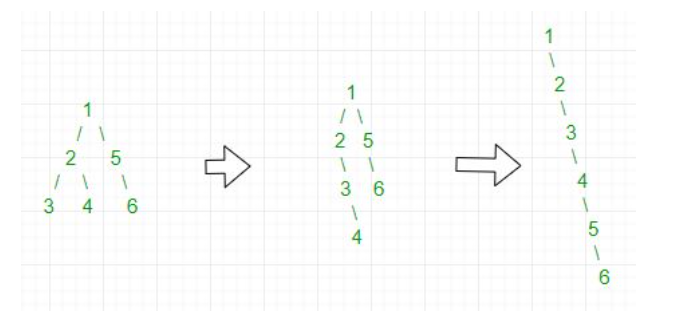
\includegraphics[scale=0.39]{pics/flat.png} \newline



\item Truncate a binary tree to remove nodes that lie on a path having a sum less than k
\begin{enumerate}
	\item Only node on a path, should use postorder. 
	\item Only print(not print) or keep(delete), should return bool
	\item calculate sum, should input a parameter sum
	\item \textbf{When delete leaf, parent will become leaf, That is why we have to use postorder}
\end{enumerate}
\begin{lstlisting}
	
void trunc(Node* &curr, int k, int sum)
{
	// base case: empty tree
	if (curr == nullptr) {
		return;
	}
	
	// update sum of nodes in the path from the root node to the current node
	sum = sum + (curr->data);
	
	// Recursively truncate left and right subtrees
	trunc(curr->left, k, sum);
	trunc(curr->right, k, sum);
	
	// Since we are doing postorder traversal, the subtree rooted at the current
	// node may be already truncated, and the current node is a leaf
	
	// if the current node is a leaf node and its path from the root node has a sum
	// less than the required sum, remove it
	if (sum < k && isLeaf(curr))
	{
		// free the memory allocated to the current node
		delete(curr);
		
		// set current node to null (node is passed by reference)
		curr = nullptr;
	}
};
\end{lstlisting}



\end{itemize}

\subsubsection{Traversal + other data structure}
\begin{itemize}
	\item Maximum Path Sum in a Binary Tree.(Global variable)
	\begin{lstlisting}[breaklines]
		For each node there can be four ways that the max path goes through the node:
		1. Node only
		2. Max path through Left Child + Node
		3. Max path through Right Child + Node
		4. Max path through Left Child + Node + Max path through Right Child
		
		The idea is to keep trace of four paths and pick up the max one in the end. An important thing to note is, root of every subtree need to return maximum path sum such that at most one child of root is involved. This is needed for parent function call. In below code, this sum is stored in 'max_single' and returned by the recursive function.
	\end{lstlisting}
\end{itemize}

\subsubsection{Other}
\begin{itemize}


\item \textbf{Idea: (recursive + return style)}

\item in order without recursive, 
\begin{lstlisting}[frame=single, language=c++]
// An iterative process to print preorder traversal of Binary tree
void iterativePreorder(node *root){
    // Base Case
    if (root == NULL)
       return;
 
    // Create an empty stack and push root to it
    stack<node *> nodeStack;
    nodeStack.push(root);
 
    /* Pop all items one by one. Do following for every popped item
       a) print it
       b) push its right child
       c) push its left child
    Note that right child is pushed first so that left is processed first */
    while (nodeStack.empty() == false)    {
        // Pop the top item from stack and print it
        struct node *node = nodeStack.top();
        printf ("%d ", node->data);
        nodeStack.pop();
 
        // Push right and left children of the popped node to stack
        if (node->right)
            nodeStack.push(node->right);
        if (node->left)
            nodeStack.push(node->left);
    }
}
\end{lstlisting}

\textbf{Idea: A common implementation of DFS, without check two unvisited condition. Because tree is a 1) minimally connected graph and having only one path between any two vertices. 2) no loop}

\item For search tree, look for lowest common ancestor(LCA). 
\begin{lstlisting}[frame=single, language=c++]
Node *LCA(Node *root, Node *p, Node *q) {
  if (!root || !p || !q) return NULL;
  if (max(p->data, q->data) < root->data)
    return LCA(root->left, p, q);
  else if (min(p->data, q->data) > root->data)
    return LCA(root->right, p, q);
  else
    return root;
}

\end{lstlisting}

\item Determine whether a binary tree is a subtree of another binary tree. both inorder and preorder together identify a tree quniquely.

\item \textbf{can be changed into a binary tree problem!}
\begin{enumerate}
	\item print all subsequence, select current or don't select
	\item stair case, walk one or two
	\item house robbery
	\item all possible combine in array. 
	
\begin{lstlisting}[frame=single, language=c++]	
Input:  digits[] = { 1, 2, 2, 1 }	
{1, 2, 2, 1} 
{1, 2, 21} 
{1, 22, 1} 
{12, 2, 1} 
{12, 21} 
\end{lstlisting}
\end{enumerate}

\end{itemize}




\section{Graph}
\subsection{Basic}
\begin{itemize}
\item \textbf{A Tree is just a restricted form of a Graph. They fit with in the category of Directed Acyclic Graphs (or a DAG). So Trees are DAGs with the restriction that a child can only have one parent.}

\item Graphs are generally search breath first or depth first. The same applies to Tree.

\item Basic represent way: \textbf{adjacency list} and \textbf{adjacency matrix}: \newline
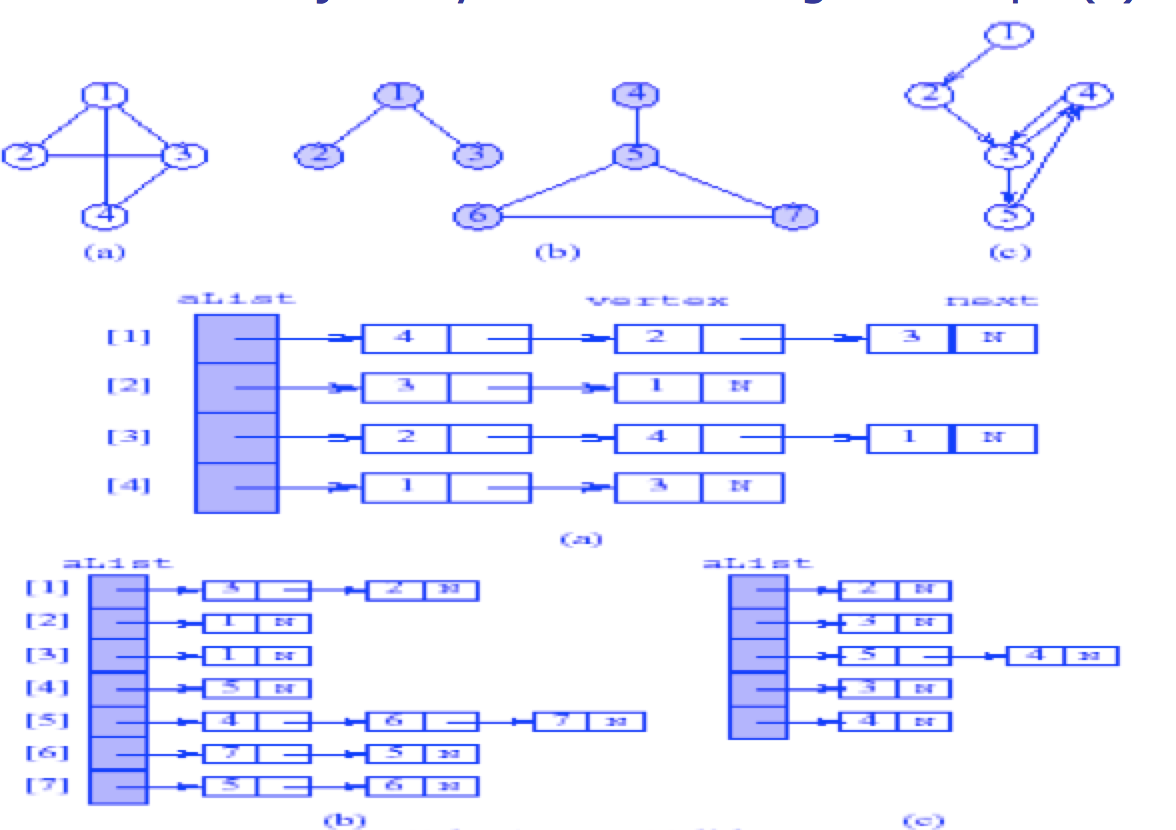
\includegraphics[scale=0.6]{pics/adjacency.png} \newline

\item You want to mirror the problem using a tree-like structure:For this we have boost graph library. The BGL currently provides two graph classes and an edge list adaptor: adjacency\_list, adjacency\_matrix and edge\_list.  The adjacency\_list class is the general purpose "swiss army knife" of graph classes.
\end{itemize}

\subsection{DFS and BFS}
\subsubsection{DFS}
\begin{itemize}
\item DFS has three versions 1) recursive 2) recursive to loop version. 3) uniform version
\begin{enumerate}
\item recursive version:
\begin{lstlisting}[frame=single, language=c++]
DFS(current){
  visit current;
  for all(next to current){
     if(unvisited(next)){
          DFS(next);
      }
   }
}
\end{lstlisting} 
\item recursive to loop
\begin{lstlisting}[frame=single, language=c++]
DFS(start){
 S.push(start)  
  while(!S.empty()){
    current = top();
    visit current;
    If (current has one unvisited next){ 
         stack.push(next);
    }   
    else{
        stack.pop()
    }
}
}
\end{lstlisting} 
\item unified version:
\begin{lstlisting}[frame=single, language=c++]
DFS(start){
 S.push(start)  
  while(!S.empty()){
    current = S.pop
    if(unvisited(current){
          visit current.
          for all(next to current and unvisited)
             S.push(next);
    }
  }
 }
\end{lstlisting} 
\end{enumerate}

\item  Why we need two "unvisited" words in DFS unified version.  
\begin{enumerate}
\item When we pop node from S, then we visit it, then we add all adjacent nodes to S, In this way, When we pop 1 from S, we add 2, 3 to S. at this time, 3 is unvisited, then when we pop 2 from S, we will add 4, 3 to S. so there are two 3 in the S. 
\item Based on, we need to first unvisit to avoid visit 3 twice

\item When we reach 3; 1,2,4 have been visited, so when we want to add all 3 adjacent, we need second unvisited to avoid 1,2,4 to S.  
\end{enumerate}
\begin{verbatim}
     1
  /    \
 2----3
 \     /
    4      
\end{verbatim}

\item DFS is an algorithm to search a hierarchical structure. But, pre-order traversal seems to be something similar also. So, what is the difference between the two?? DFS says:
\begin{enumerate}
\item If element found at root, return success.
\item If root has no descendants, return failure
\item Recursive DFS on left subtree: success if element found
\item If not, Recursive DFS on right subtree: success if element found
\end{enumerate}
Pre-order Traversal says:
\begin{enumerate}
\item Visit the root
\item Recursive pre-order on left subtree
\item Recursive pre-order on right subtree
\end{enumerate}

\end{itemize}

\subsubsection{BFS}

\begin{itemize}
\item There are two version of BFS:
\begin{enumerate}
\item Form DFS unify version, We can change S(stack) to Q(queue) and get unified version. \textbf{That is why we call it unified version}
\begin{lstlisting}[frame=single, language=c++]
BFS(start){
 Q.push(start)  
  while(!Q.empty()){
    current = Q.pop
    if(unvisited(current){
          visit current.
          for all(next to current and unvisited)
             Q.push(next);
    }
  }
 }
\end{lstlisting} 
\item Common version:  Unified version will have multi-copy vertex in the queue. We can improve it as below:  1) when you add it to queue, visit it. In this way, avoid add multi-copy vertex in queue 2) Because All the vertex in queue is visited, when you pop it, you don't need to judge if it's visisted. 
\begin{lstlisting}[frame=single, language=c++]
DFS(start){
 D.push(start)  
  while(!D.empty()){
    current = D.pop  //2) no if here
    for all(next to current and unvisited){
         visit current.  //1) push and visit at the same time. 
         D.push(next);
     }
  }
 }
\end{lstlisting} 

\item conclusion:
\begin{enumerate}
\item  \textbf{Conclusion, just remember unified version. 1) pop current, push neighbor, 2) check two unvisited}
\item unified version will push two nodes into stack or queue, so for BFS, you can visit and push at the same time, in this way, you don't need to check current if it is unvisited. 

\item For DFS, you can't use this way, because you can only visit only one neighbor, or it will become BFS. so each time, you just push one node into stack. It leads to two other versions. recursive version, and loop version. 
\end{enumerate}


\end{enumerate}

\item Path is saved in the stack.  when you quit while loop. just pop up each position from stack, then you get a path. But for BFS, you need extra information to save parent information. 
\end{itemize}

\subsection{spanning tree}
\begin{itemize}
\item 	BFS and DFS will produce spanning tree. 
\item The minimum spanning tree can be obtained in polynomial time:
\begin{enumerate}
\item Kruskal's algorithm
\item Prim's algorithm
\item Sollin's algorithm
\end{enumerate}

\item Kruskal algorithm:
\begin{lstlisting}[frame=single, language=c++]
KRUSKAL(G):
 A = empty
 foreach v in G.V:
    MAKE-SET(v)
 foreach (u, v) ordered by weight(u, v), increasing:
    if FIND-SET(u) != FIND-SET(v):
       A = A  {(u, v)}
       UNION(u, v)
 return A
\end{lstlisting}
\begin{description}
	\item[Source code:] union find algorithm.
\end{description}

\end{itemize}


\subsection{Application}
\begin{itemize}
\item detect a cycle in the graph. \textbf{Undirected graph, not directed graph}
\begin{lstlisting}[frame=single, language=c++]
// A recursive function that uses visited[] and parent to detect
// cycle in subgraph reachable from vertex v.
bool Graph::isCyclicUtil(int v, bool visited[], int parent){
    // Mark the current node as visited
    visited[v] = true;
 
    // Recur for all the vertices adjacent to this vertex
    list<int>::iterator i;
    for (i = adj[v].begin(); i != adj[v].end(); ++i){
        // If an adjacent is not visited, then recur for that adjacent
        if (!visited[*i])        {
           if (isCyclicUtil(*i, visited, v))
              return true;
        }
        // If an adjacent is visited and not parent of current vertex,
        // then there is a cycle.
        else if (*i != parent)
           return true;
    }
    return false;
}
\end{lstlisting}

\begin{center}
		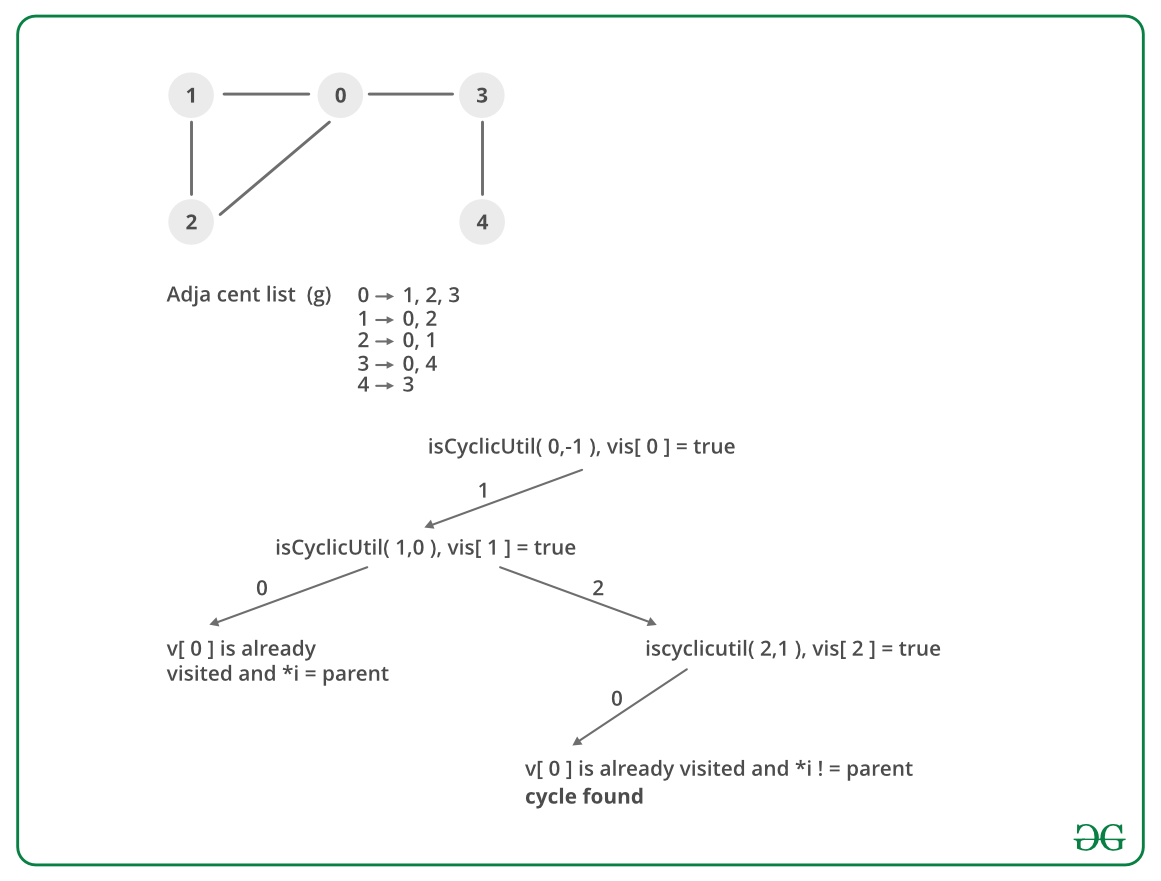
\includegraphics[width=0.7\linewidth]{pics/dc.png}
\end{center}

	\item direct graph detect cycle. \textbf{need to add a onPath to detect cycle, different with undirected graph.}
\begin{lstlisting}
boolean[] onPath;
boolean[] visited;

boolean hasCycle = false;

void traverse(List<Integer>[] graph, int s) {
	if (onPath[s]) {
		// find cycle
		hasCycle = true;
	}
	if (visited[s] || hasCycle) {
		return;
	}

	visited[s] = true;

	onPath[s] = true;
	for (int t : graph[s]) {
		traverse(graph, t);
	}
	onPath[s] = false;
}
\end{lstlisting}

\end{itemize}

\section{other customized data structure}

\subsection{union find}

\begin{itemize}
	\item it is also called as "Online Equivalence class"
	
	\item definition of Equivalence relationship
	\begin{enumerate}
		\item a ~ a. (Reflexivity)
		\item a ~ b if and only if b ~ a. (Symmetry)
		\item if a ~ b and b ~ c then a ~ c. (Transitivity)
	\end{enumerate}
	
	\item online equivalence class, also known union-find question.  
	\begin{enumerate}
		\item method 1: use array  \newline 
		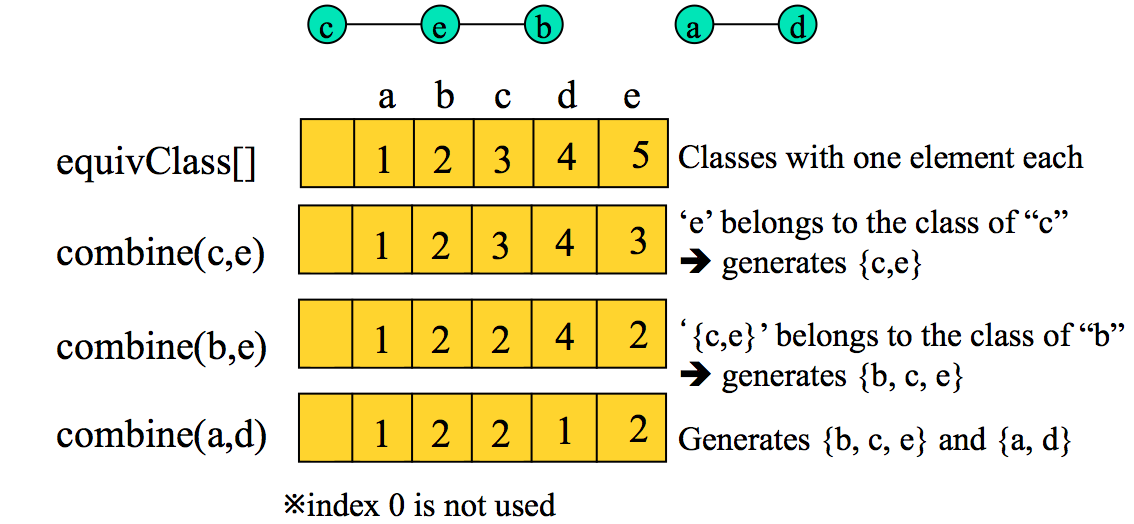
\includegraphics[scale=0.55]{pics/online_1.png} 
		
		\item method 2: stimulate pointer \newline 
		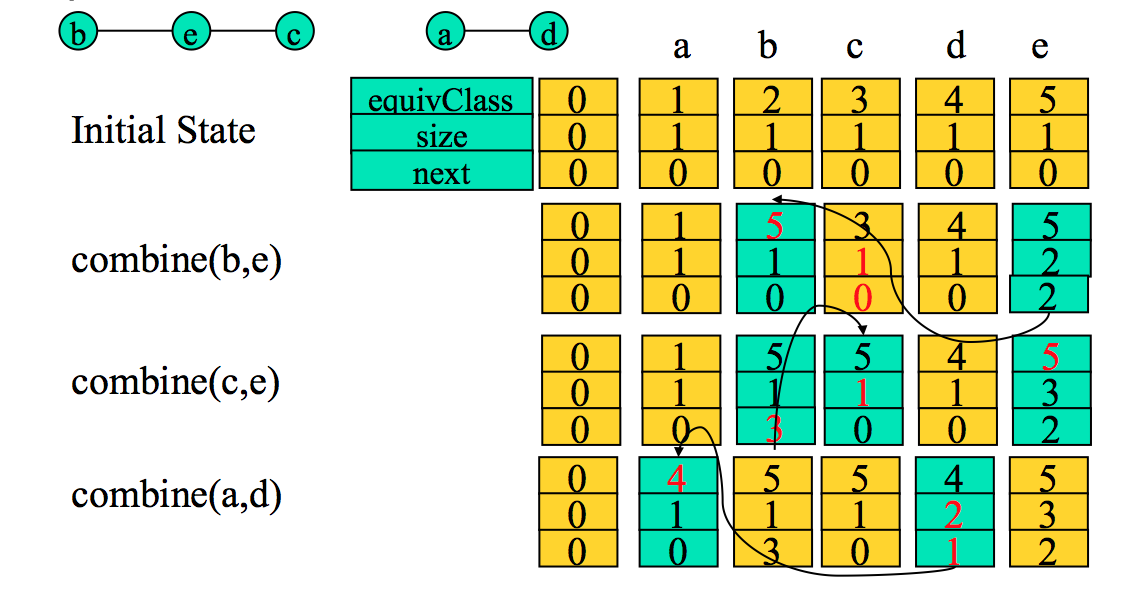
\includegraphics[scale=0.55]{pics/online_2.png}  
	\end{enumerate}
	
\end{itemize}
	
\subsection{LRU and LFU}
\begin{itemize}
	\item  LRU is hash + list. (listedhashmap)
	\item  LFU is hash + heap.
	\item In LRU and LFU, The key data structure is LinkedHashMap, in LFU, it use LinkedSetMap, in fact, LinkedSetMap still use the LinkedHashMap behind the scene. 
\begin{center}
	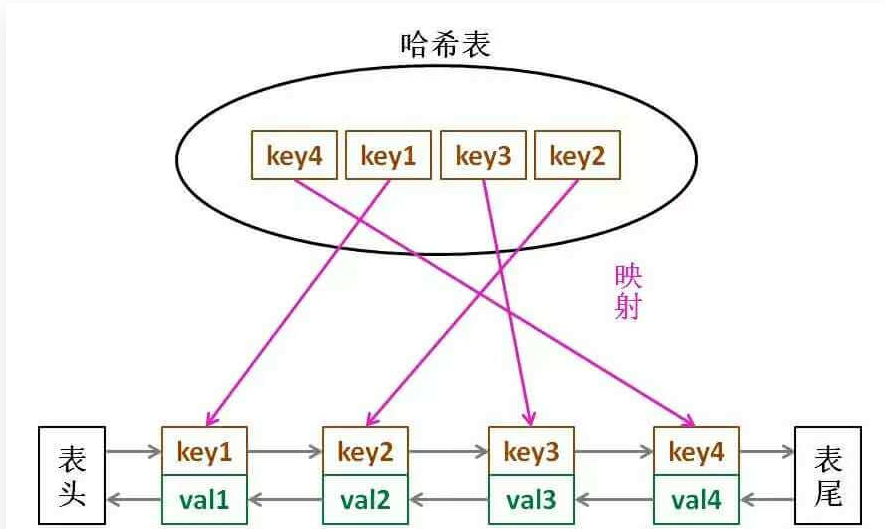
\includegraphics[width=0.7\linewidth]{pics/LinkedHashMap}
\end{center}
	


\end{itemize}

	
\subsection{O(1) insert, delete and get}
insert, delete get random O(1)  hash +vector(no need to keep vector sort)
	

\chapter{Algorithm}
\section{Math and geometry basic}
\subsection{geometry}
\begin{itemize}
\item Judge three points are in the same line?
\[
\dfrac{y_{2}-y_{1}}{x_{2}-x_{1}}  = \dfrac{y_{3}-y_{1}}{x_{3}-x_{1}}
\]

\item Get one points in the triangle. 

\[
x = \dfrac{\dfrac{x_{1}+x_{2}}{2}+x_{3}}{2}
\]

\item If two rectangles overlap?
\begin{verbatim}
l1: Top Left coordinate of first rectangle.
r1: Bottom Right coordinate of first rectangle.
l2: Top Left coordinate of second rectangle.
r2: Bottom Right coordinate of second rectangle.

1) One rectangle is above top edge of other rectangle.
2) One rectangle is on left side of left edge of other rectangle.
\end{verbatim}

\begin{lstlisting}[frame=single, language=c++]
// Returns true if two rectangles 
//(l1, r1) and (l2, r2) overlap
bool doOverlap(Point l1, Point r1, Point l2, Point r2){
    // If one rectangle is on left side of other
    if (l1.x > r2.x || l2.x > r1.x)
        return false;
    // If one rectangle is above other
    if (l1.y < r2.y || l2.y < r1.y)
        return false;
    return true;
}
\end{lstlisting}

\end{itemize}

\subsubsection{convex hull}

\begin{enumerate}
\item Find a point C that is inside the convex hull of S
( (sum of x coordinates)/ n, (sum of y coordinates)/n )
\item Sort S by polar angle and within polar angle by distance from C. Use atan2(y-Cy , x-Cx) c++ function.
\item Create a doubly linked circular list of points using above order
Let right link to the next point in the order and left link to the previous point

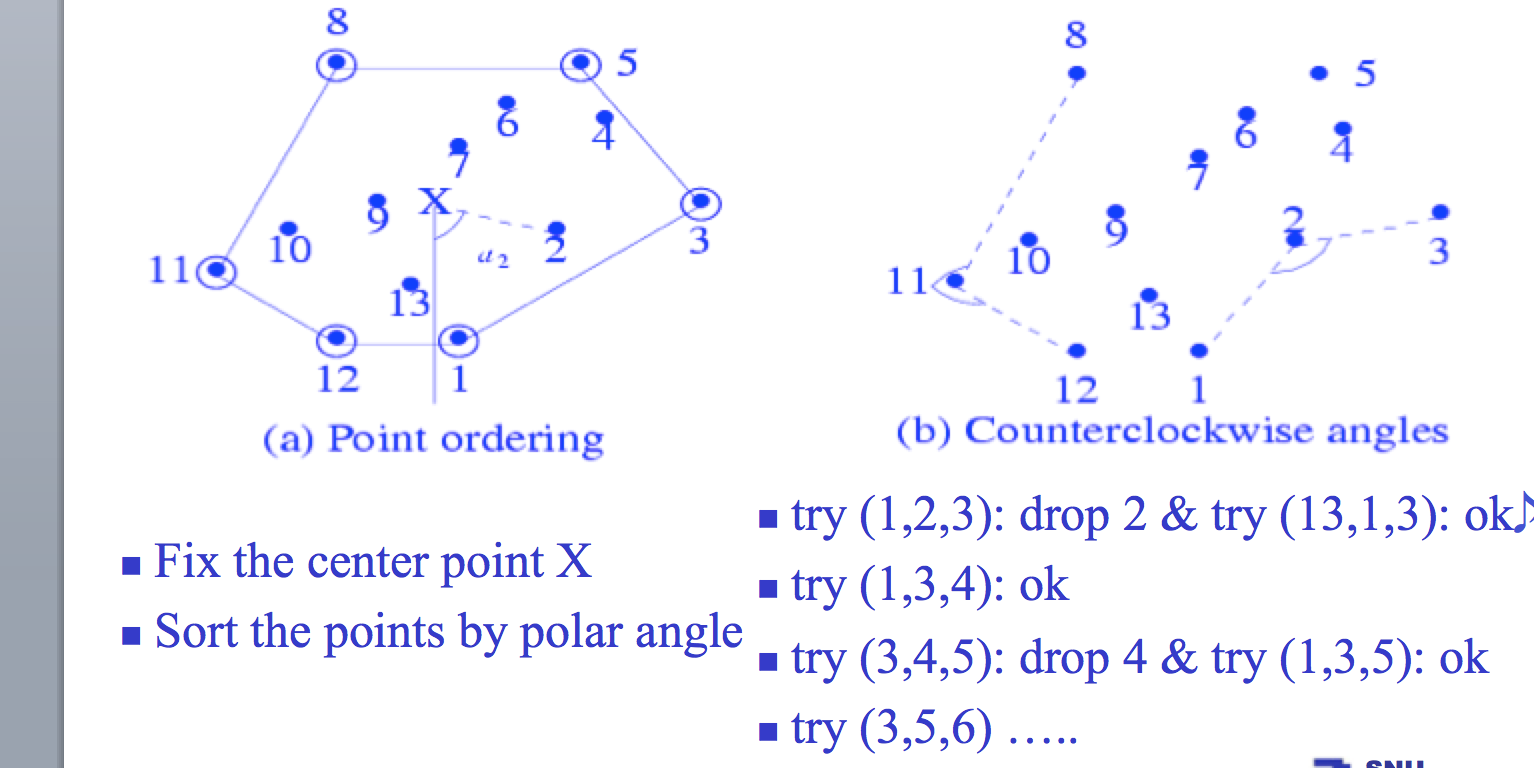
\includegraphics[scale=0.4]{pics/convex.png} \newline
\item Let p be the point that the smallest y-coordinate 
   (break a tie, if any, by selecting the one with largest x-coordinate)
   
\item use Law of cosines to calculate  angle formed by x, rx and rrx
\[
c^{2} = a^{2}+b^{2}-2ab\cos\lambda
\]

\begin{lstlisting}[frame=single, language=c++]
 for (x = p; rx = point to the right of x; x != rx) {
       rrx = point to the right of rx;
       if (angle formed by x, rx, and rrx is <=180 degrees) {
           delete rx from the list;
           rx = x; 
           x = point on left of rx;
       } 
       else { 
       x = rx; rx = rrx;}
   } 
\end{lstlisting}

\item For convex hull problem, you can use double link list to store all the extreme points. Because it need to use three consequence points to measure the degree to judge if it's less than 180 degrees. So double link list is the best data structure to use. 

\end{enumerate}


\subsection{Permutation and combination}
\begin{itemize}
\item repeated / unrepeated (Permutation/Combination)

\item repeated permutation: Three number, how many permutation $10^3$. Another Three position, For each position, you can select 10 options and fill it.  If three position, For each position, you can selet 2 options and fill it. You get powerset problem $2^3$ \{a,b, c\} all the subset. 

\item unrepeated permutation: $n! = factorial function$
\item unrepeated combination:  
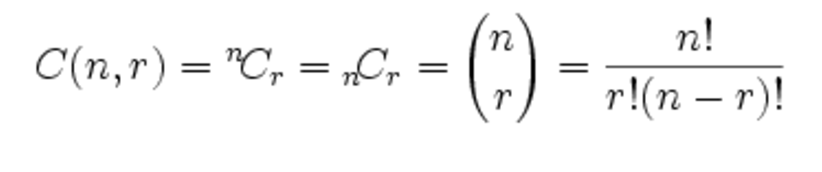
\includegraphics[scale=0.6]{pics/UC.png} \newline
\item repeated combination: 
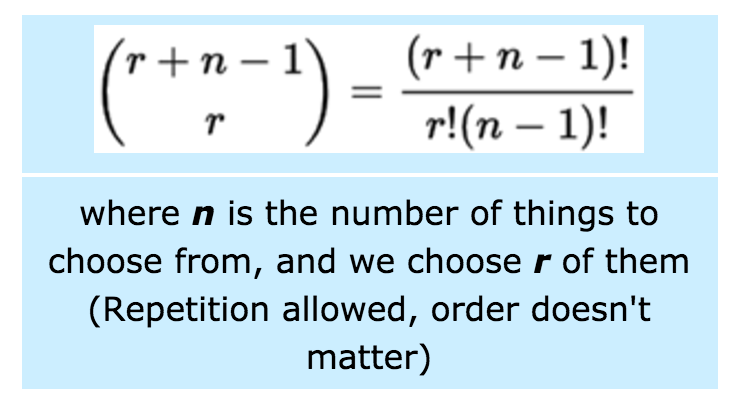
\includegraphics[scale=0.6]{pics/RC.png} \newline
\item detail can been seen here: https://www.mathsisfun.com/combinatorics/combinations-permutations.html

\end{itemize}

\subsection{solution space }
\begin{itemize}
	\item why this basic conception is so important, Because you can use these four to describe solution space. repeated permutation can be use in 0/1 backpack problem.  LCS problem.  

	\item nearest point pair's solution space is n*(n-1). It's $n^2$. A good hint is that it can be reduce $n*log(n)$. So We should consider D\&C (divide and conquer)

	\item 0/1 packback's solution's space is $2^n$, A good hint is that I can be reduce to $n^c$. (c is constant) by dynamic programming. 

	\item If there is not D\&C or DP, you have to use branch and bound or backtracking.  such as TSP travelling sales problem

	\item If you need optimal answer, You need to traversal the whole solution space. ( such as TSP and 0/1 backpacking). If you don't need optimal answer, you don't need to do that, In these two conditions, you all need to \textbf{backtracking.}

\item Why I can't use DP to TSP, but I can use DP to 0/1?  

\end{itemize}

\begin{itemize}

\item recursion is a mathematical induction. 
\item modeling is mapping your problem to a abstract structure.
\begin{enumerate}
\item Permutation: arrangement, tour,ordering sequence
\item subset: cluster, collection, committee, group, packaging, selection
\item tree:hieracrchy, dominance, ancestor/descendant, taxonomy
\item graphs: network, circuit, web, relationship
\item points
\item polygon
\item string 
\end{enumerate}

\end{itemize}

\subsection{bit}
\begin{itemize}
	\item Basic operations are: and, or, xor, not, right shift, left shit. 
\begin{lstlisting}[frame=single, language=c++]	
number |= 1UL << n; // set
number &= ~(1UL << n); //clear
number ^= 1UL << n;  //toggle
\end{lstlisting}

	\item Many C compilers choose which right shift to perform depending on what type of integer is being shifted; often signed integers are shifted using the arithmetic shift, and unsigned integers are shifted using the logical shift.
	
\begin{lstlisting}[frame=single, language=c++]	
a|b|c|d //after we right shift, we change it to below
x|a|b|c
1) with a logical shift put 0 in x
2) with a arithmetic shift put a in x
\end{lstlisting}	
	
	\item XOR is exclusive or, You can think that it's subset of OR, for OR, if both bits are 1, the result is 1. but In XOR, we exclusive this possible,  You can think that it's "pure" or.  Based on previous definition. There are two characteristics:
\begin{lstlisting}
x^x = 0
x^0 = x
\end{lstlisting}
	from previous two examples, we can use it to find any number occur even number in the array. 
		
	\item change the last 1 to zeor. The basic idea is very interesting. 
	\begin{lstlisting}[frame=single, language=c++]	
		n&(n-1);
		//110100-> 110000
		
		//when we n-1: 110100, the right most 1 will become 0, all zeor after 
		//right most 1 will become 1. 
		110100
		110011
		*--
	\end{lstlisting}
	
	\item Based on previous trip, we can test if a number is power of 2. There is only one 1 in the binary formation.
	\begin{lstlisting}[frame=single, language=c++]	
		bool isPowerOfTwo(int n) {
			if (n <= 0) return false;
			return (n & (n - 1)) == 0;
		}	
	\end{lstlisting}
	
	\item Hamming weight,  Hamming weight of an integer is defined as the number of set bits in its binary representation. 
	\begin{lstlisting}[frame=single, language=c++]	
		int hammingWeight(uint32_t n) {
			int res = 0;
			while (n != 0) {
				n = n & (n - 1); //change n, you need to assign new value back to n. 
				res++;
			}
			return res;
		}
	\end{lstlisting}

	\item As noted in this answer, n\&(n-1) unsets the last set bit.
So, if we unset the last set bit and xor it with the number; by the nature of the xor operation, the last set bit will become 1 and the rest of the bits will return 0
\begin{lstlisting}
	int set_bit = n ^ (n&(n-1));
\end{lstlisting}


\end{itemize}

\subsection{Usage of model \%}

\begin{itemize}
\item circular queue
\item hash
\item to know the last three digit. 
\end{itemize}

\section{two pointers}

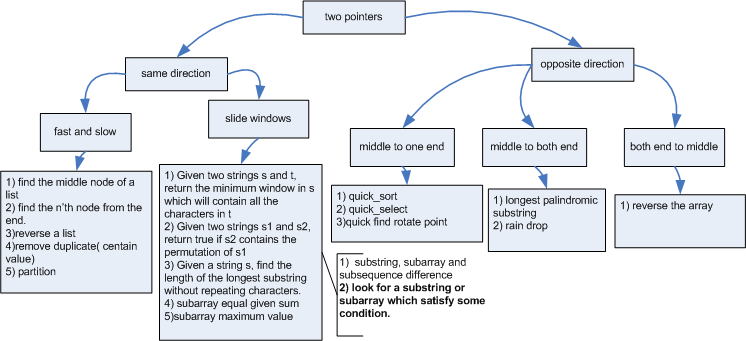
\includegraphics[scale=0.6]{pics/two_pointers.png} \newline




\subsection{middle to both ends}
\begin{itemize}
	\item the longest palindrome substring
	
\begin{lstlisting}[breaklines]
string palindrome(string& s, int l, int r) {
	// check if it out boundary
	while (l >= 0 && r < s.size()
	&& s[l] == s[r]) {
		// both side move
		l--; r++;
	}
	// return result
	return s.substr(l + 1, r - l - 1);
}

string longestPalindrome(string s) {
	string res;
	for (int i = 0; i < s.size(); i++) {
		// s[i] is middle
		string s1 = palindrome(s, i, i);
		// s[i] and s[i+1] 
		string s2 = palindrome(s, i, i + 1);
		// res = longest(res, s1, s2)
		res = res.size() > s1.size() ? res : s1;
		res = res.size() > s2.size() ? res : s2;
	}
	return res;
}
\end{lstlisting}
	
	\item rain drop
	
\begin{lstlisting}[breaklines]
int trap(vector<int>& height) {
	if (height.empty()) return 0;
	int n = height.size();
	int res = 0;
	// memo
	vector<int> l_max(n), r_max(n);
	// base case
	l_max[0] = height[0];
	r_max[n - 1] = height[n - 1];
	// calculate l_max from left to right
	for (int i = 1; i < n; i++)
	l_max[i] = max(height[i], l_max[i - 1]);
	// calculate r_max from right to left
	for (int i = n - 2; i >= 0; i--) 
	r_max[i] = max(height[i], r_max[i + 1]);
	
	// calculate the last answer.
	for (int i = 1; i < n - 1; i++) 
	res += min(l_max[i], r_max[i]) - height[i];
	return res;
}
\end{lstlisting}

\end{itemize}


\subsection{slow and fast}
\begin{itemize}
	\item remove duplicate
\begin{lstlisting}[breaklines]
int removeDuplicates(int[] nums) {
	if (nums.length == 0) {
		return 0;
	}
	int slow = 0, fast = 0;
	while (fast < nums.length) {
		if (nums[fast] != nums[slow]) {
			slow++;
			// maintain nums[0..slow] without duplicate
			nums[slow] = nums[fast];
		}
		fast++;
	}
	// length should be  + 1
	return slow + 1;
}
\end{lstlisting}

	\item partition
\begin{lstlisting}[breaklines]
template<class ForwardIt, class UnaryPredicate>
ForwardIt partition(ForwardIt first, ForwardIt last, UnaryPredicate p)
{
	first = std::find_if_not(first, last, p);
	if (first == last) return first;
	
	for (ForwardIt i = std::next(first); i != last; ++i) {
		if (p(*i)) {
			std::iter_swap(i, first);
			++first;
		}
	}
	return first;
}
\end{lstlisting}
% remove and partition has the same idea, remove uses overwrite, partition uses swap, that is all. 
	
\end{itemize}
\subsection{slide windows}
\begin{itemize}
	\item Code template
\begin{lstlisting}[breaklines]
	int left = 0, right = 0;
	
	while (right < n) {`
		// increase windows
		window.add(a[right]);
		right++;
		
		//update windows
		//.......
		
		while (window needs shrink) {
			// decrease window
			window.remove(s[left]);
			left++;
			
			//update windows here.
			//......
		}
	}			
\end{lstlisting}

	\item An example. minimal substring in source which includes all the letters of in target.
	s = "ADOBECODEBANC", t = "ABC, output "BANC"
\begin{lstlisting}[breaklines]
	int left = 0, right = 0;
	
	while (right < n) {`
		// increase windows
		window.add(a[right]);
		right++;
		
		//update windows
		//.......
		
		while (window needs shrink) {
			// decrease window
			window.remove(s[left]);
			left++;
			
			//update windows here.
			//......
		}
	}			
\end{lstlisting}

		
\end{itemize}


\section{Recursive}
\subsection{Basic}
\begin{itemize}

	\item recursive is not an algorithm, it's just a method. D\&C, DP, backtrack, bound and boundary all use recursive in their implementation, but different ways. 
	
	\item First, the inline specification on a function is just a hint. The compiler can (and often does) completely ignore the presence or absence of an inline qualifier. With that said, a compiler can inline a recursive function, much as it can unroll an infinite loop. It simply has to place a limit on the level to which it will "unroll" the function.

	\item One recursive(Factorial),  Two recursive call( Hanoti) (Tree), Multi Recursive(Permutation)

	\item result is single (FActorial), Result is many steps,(Hanoti) (Maze), Result is a set( permutation). you can see that 1) any recursive function should at least one input parameter, and this parameter should to be pass sub-problem. 2) for return value, it has two different kind, if result is single value, you should return a value, such as Factorial. If result is set(permutation) or many steps(in-order traversal of treeor Hanoi tree), you can declare your function as void. 3) Some functions need input another parameter, such as level information in the tree or position information in the permutation. 4) Base case can be understood differently, most of time base case is 0 or null, but for permutation, base case is i==n.  most subproblem, i decrease, but for permutation, for each subproblem i increase. 
\begin{enumerate}
\item single result 
\begin{lstlisting}[frame=single, language=c++]
int Factorial(int n){
if (n == 1) 
     return 1;
 return n*Factorial(n-1);
}
\end{lstlisting}

	\item result is serial steps (Hanoti) DFS(Maze)
\begin{lstlisting}[frame=single, language=c++]
FUNCTION MoveTower(disk, source, dest, spare):
IF disk == 0, THEN:
    move disk from source to dest
ELSE:
    MoveTower(disk - 1, source, spare, dest)   // Step 1 above
    move disk from source to dest              // Step 2 above
    MoveTower(disk - 1, spare, dest, source)   // Step 3 above
END IF
\end{lstlisting}
Result is a set( permutation)

\end{enumerate}

	\item It includes direct recursive and indirect recursive. direct recursive is R() call R() again in it's funciton body. It has two parts: \textbf{1)base and 2) recursive component}
	
\subsection{basic recursive pattern}
\begin{itemize}
	\item You should understand Big O here. for example 
	\begin{enumerate}
		\item O(n) is found max and min
		\item O(n*n) is sort
		\item O(n*n*n) is  solutions for a multi-variable equation. such as 3x+4y+5z = 108, then get all x, y z.
		\item O(n*logn) is quick sort. binary search. 
		\item O($2^{n}$) print all subsequences
		\item catalan number. print all parentheses.
		\item O($n!$) print all permutation.
		
	\end{enumerate}
		
	\item print all subsequences, why is power(2,n)?
	\begin{lstlisting}[frame=single, language=c++]
		void sub(string& s, int i, int j, string res) {
			
			if (i == j) {
				cout << res << endl;
				return;
			}
			//don't select current character
			sub(s, i + 1, j, res);
			
			//select current character.
			res.push_back(s[i]);
			sub(s, i + 1, j, res);
		}
	\end{lstlisting}
	
	\item A similar idea is to LIS problem. it's also power(2,n)
	you can think in this way, previous one is 2*f(n-1), below is f(n-1) f(n-2)...f(1)
	but f(n-2)...f(1) is just another f(n-1), so equal 2*f(n-1). Detail is we have a lot of overlap problem.
	Time complexity is power(2,n) The time complexity of this recursive approach is exponential as there is a case of overlapping subproblems as explained in the recursive tree diagram above.
	\begin{center}
		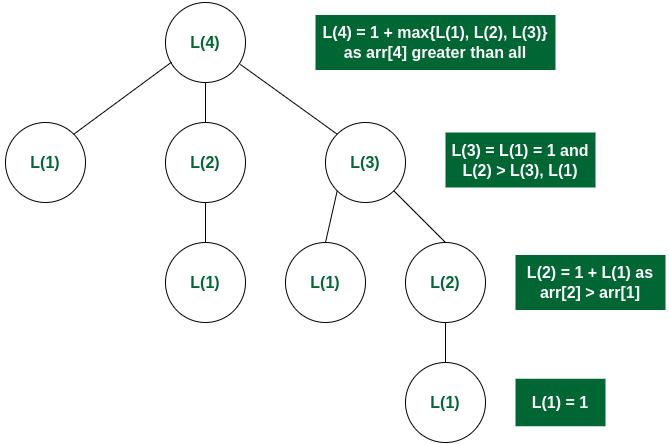
\includegraphics[width=0.7\linewidth]{pics/lis}
	\end{center}
	
	\begin{lstlisting}[frame=single, language=c++]
		int _lis( int arr[], int n, int *max_ref)
		{
			/* Base case */
			if (n == 1)
			return 1;
			
			// 'max_ending_here' is length of LIS
			// ending with arr[n-1]
			int res, max_ending_here = 1;
			
			/* Recursively get all LIS ending with arr[0],
			arr[1] ... arr[n-2]. If arr[i-1] is smaller
			than arr[n-1], and max ending with arr[n-1]
			needs to be updated, then update it */
			for (int i = 1; i < n; i++)
			{
				res = _lis(arr, i, max_ref);
				if (arr[i-1] < arr[n-1] && res + 1 > max_ending_here)
				max_ending_here = res + 1;
			}
			
			// Compare max_ending_here with the overall
			// max. And update the overall max if needed
			if (*max_ref < max_ending_here)
			*max_ref = max_ending_here;
			
			// Return length of LIS ending with arr[n-1]
			return max_ending_here;
		}
	\end{lstlisting}
	
	
	\item If the answer is one, such as LIS, the result should be in the root node, we should use post order, If the answer are a lot , the result shoudl be in leaf node, we should use base case. such as all possible subsequence. 
	
	\item catalan number, all possible parentheses combination. (It's not good implementation, some child problems have been calcualted many time.  You should use dynamic programming to remember the child problems result. but child program result is very big.  It's a question for ALL , not for ONE result. So backtrace algorithm is more good for this questions. 
	
	\item Re-interpreting the symbol X as an open parenthesis and Y as a close parenthesis, Cn counts the number of expressions containing n pairs of parentheses which are correctly matched:
	\begin{lstlisting}
		((()))     (()())     (())()     ()(())     ()()()
	\end{lstlisting}
	
	Cn is the number of different ways n + 1 factors can be completely parenthesized (or the number of ways of associating n applications of a binary operator, as in the matrix chain multiplication problem). For n = 3, for example, we have the following five different parenthesizations of four factors:
	
	\begin{lstlisting}	
		((ab)c)d     (a(bc))d     (ab)(cd)     a((bc)d)     a(b(cd))
	\end{lstlisting}
	
	\begin{lstlisting}[frame=single, language=c++]
		vector<string> ap(string& s, int i, int j) {
			vector<string> result;
			if (i == j-1 && i<s.size()) {
				result.push_back("("+s.substr(i,1)+")");
				return result;
			}
			if (i == j - 2 && i<s.size()-1) {
				result.push_back("(" + s.substr(i, 2) + ")");
				return result;
			}	
			for (int k = i; k < j-1; ++k) {
				vector<string> v1 = ap(s, i, k+1);
				vector<string> v2 = ap(s, k+1 , j);
				
				string rs;
				for (auto e : v1) {
					for (auto e1 : v2) {
						rs =  e;
						rs += e1;
						result.push_back(rs);
					}
				}
			}
			return result;
		}
		
		string s = "abcd";
		auto com = ap(s, 0, 4);
		
		for (auto e : com) {
			cout << e << endl;
		}
		
		(a)(b)(cd)
		(a)(bc)(d)
		(ab)(cd)
		(a)(bc)(d)
		(ab)(c)(d)
	\end{lstlisting}
	
	\item The same idea is to build binary search tree
	\begin{lstlisting}[frame=single, language=c++]
		// Recursive function to return a list of tree pointers of all possible
		// binary trees having the same inorder sequence as `in[start, end]`
		vector<Node*> generateBinaryTrees(vector<int> &in, int start, int end)
		{
			// create an empty list to store the root of the constructed binary trees
			vector<Node*> trees;
			
			// base case
			if (start > end)
			{
				trees.push_back(nullptr);
				return trees;
			}
			
			// consider each element in the inorder sequence as the root
			for (int i = start; i <= end; i++)
			{
				// recursively find all possible left subtrees for root `i`
				vector<Node*> left_subtrees = generateBinaryTrees(in, start, i - 1);
				
				// recursively find all possible right subtrees for root `i`
				vector<Node*> right_subtrees = generateBinaryTrees(in, i + 1, end);
				
				// do for each combination of left and right subtrees
				for (Node* l: left_subtrees)
				{
					for (Node* r: right_subtrees)
					{
						// construct a binary tree with i'th element as the root and whose
						// left and right children point to `l` and `r`, respectively
						Node* tree = new Node(in[i], l, r);
						
						// add this tree to the output list
						trees.push_back(tree);
					}
				}
			}
			
			return trees;
		}
	\end{lstlisting}
	
	
	
	
\end{itemize}

%这部分很重要。主要是求所有的子集, 这个问题可以解释很多的问题,就像01背包也是一个所有子集的问题,一个lis也是所有子集的问题。 
\begin{lstlisting}
	void subset(int arr[], vector<int>& result, int k) {
		if (k == 6) {
			cout << "one answer is ( ";
			for (int i = 0; i < result.size(); i++) {
				cout << result[i] << " ";
			}
			cout << ")" << endl;
			return;
		}
		result.push_back(arr[k]);
		subset_bucket(arr, result, k + 1);
		result.pop_back();
		subset_bucket(arr, result, k + 1);
		return;
	}
\end{lstlisting}

	\item permutation, It is also worth noting that when you make a recursive call, you advance down an individual branch of the tree, and an additional branch is added with every iteration of a 'for' or 'while' loop. One confusing thing about this problem is the second swap after the recursive call to permute. This can be interpreted as 'unswap,' and is required because the char array is passed by reference, not by value, and every time you swap elements in the array the change is visible down stream.


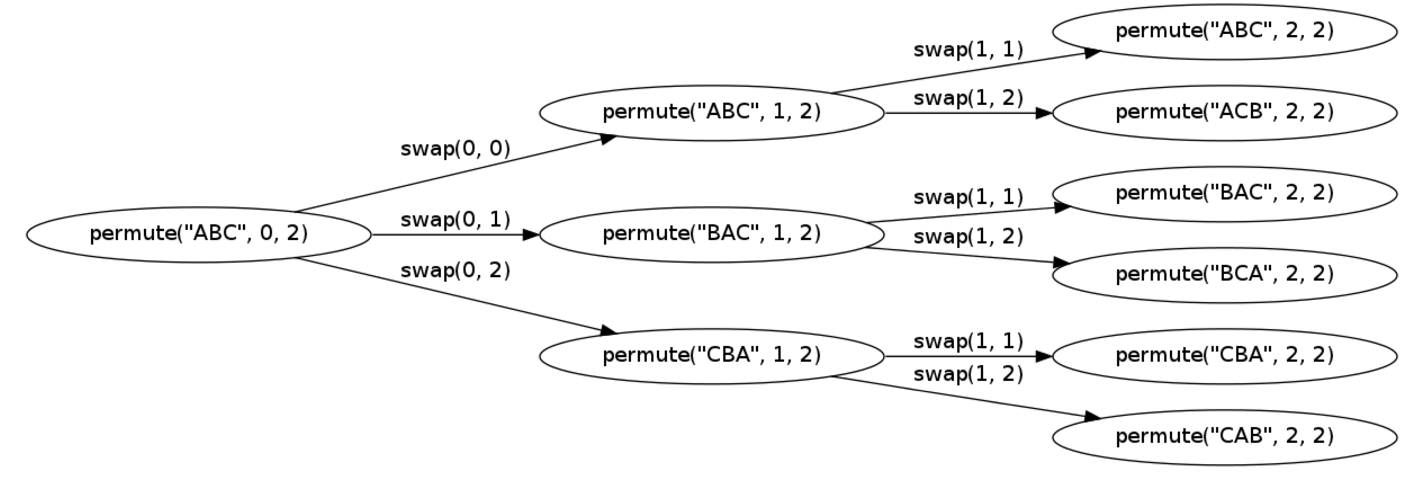
\includegraphics[scale=0.25]{pics/permutation.png}


\begin{lstlisting}[frame=single, language=c++]
	void permute(char a[], int i, int n){
		int j;
		if (i == n)
		cout << a << endl;
		else   {
			for (j = i; j <= n; j++)       {
				swap(a[i], a[j]);          
				permute(a, i+1, n);
				swap(a[i], a[j]);
			}
		}
	} 	
\end{lstlisting}

compared with subset code, You will find that they are all recursive. permutation is n!
\begin{lstlisting}
	permute(i)
	for(j...)  //calculate j times same size(i+1) sub problem.
	permute(i+1)  //similar with n*f(n-1)
	
\end{lstlisting}


\end{itemize}

\section{Sort}
\subsection{Kth element}
\begin{itemize}
	\item There is a few options:
	\begin{enumerate}
		\item n*log(n) sort
		\item n*k partial insert 
		\item n*log(k) heap 
		\item O(n) median of medians 
	\end{enumerate}

	\item \textbf{basic idea is quick select, but we use median of median method to get good pivot, to make at the worst 30-70 partition.}
	
	\item stable\_partition.
\begin{lstlisting}
#include <algorithm>

template <typename Iterator, typename Predicate>
Iterator my_stable_partition(Iterator first, Iterator last,
Predicate predicate) {
	auto n = std::distance(first, last);
	if (n <= 1) {
		if (n == 1 && predicate(*first))
		++first;
		return first;
	}
	auto middle = first;
	std::advance(middle, n / 2);
	auto a = my_stable_partition(first, middle, predicate);
	auto b = my_stable_partition(middle, last, predicate);
	return std::rotate(a, middle, b);
}	
\end{lstlisting}
	
	\item median of medians
\begin{lstlisting}[frame=single, language=c++, basicstyle=\scriptsize]
int array[] = { 1,12,3,4,1,      5,2,7,8,88,      5,2,32,1,35,   -1,7,5,38,-11 };

int insertSort(int left, int right) {
	for (int i = left + 1; i <= right; i++) {
		int temp = array[i], j;
		for (j = i; j > left && array[j - 1] > temp; j--) array[j] = array[j - 1];
		array[j] = temp;
	}
	return (left + right) >> 1;
}

int BFPRT(int, int, int);

int getPivotIndex(int left, int right) {
	if (right - left < 5) return insertSort(left, right);
	int back = left - 1;
	for (int i = left; i + 4 < right; i += 5) {
		std::cout << "i" << i <<" "<< right<<std::endl;
		int index = insertSort(i, i + 4);
		std::swap(array[++back], array[index]);
	}
	return BFPRT(left, back, ((left + back) >> 1) + 1);
}


int partition(int left, int right, int pivotIndex) {
	std::swap(array[right], array[pivotIndex]);
	int mid = left;
	for (int i = left; i < right; i++) {
		if (array[i] < array[right])
		std::swap(array[i], array[mid++]);
	}
	std::swap(array[right], array[mid]);
	return mid;
}

int BFPRT(int left, int right, int k) {
	int pivotIndex = getPivotIndex(left, right);
	int mid = partition(left, right, pivotIndex);
	int count = mid - left + 1;
	if (count == k) {
		return mid;
	}
	else if (count > k) {
		return BFPRT(left, mid - 1, k);
	}
	else {
		return BFPRT(mid + 1, right, k - count);
	}
}

int main() {
	int k = 5;
	int length = sizeof(array) / sizeof(array[0]);
	for (int i = 0; i < length; i++) {
		std::cout << array[i] << "  ";
	}
	std::cout << std::endl << " " << k << " ";
	std::cout << array[BFPRT(0, length - 1, k)] << std::endl;
	return 0;
}
	
\end{lstlisting}

\end{itemize}

\subsection{Simple sort}
\begin{itemize}
	\item Write Max and Insert functions to help to organize your algorithm
	\item All sort algorithm don't compare equal relationship. So some algorithm is Stable, and other is not stable
	\item Bubble is simple source code stable sorting. 
	\item All the sorting is from minimum to maximum.
\end{itemize}
 
\begin{enumerate}
	\item for all sort comparsion, there is good ref website: https://www.toptal.com/developers/sorting-algorithms/selection-sort

	\item Selection sort is an in-place comparison sort. O(n2). The algorithm finds the minimum value, swaps it with the value in the first position.  And repeat From the comparisons presented here, one might conclude that selection sort should never be used. It does not adapt to the data in any way (notice that the four animations above run in lock step), so its runtime is always quadratic. However, selection sort has the property of minimizing the number of swaps. In applications where the cost of swapping items is high, selection sort very well may be the algorithm of choice. Selection sort only need O(n) write, so if write is expensive operation, you need to use it. 
\begin{lstlisting}[frame=single, language=c++]
For(int size=n ;size>1;size--){
Int j = Max(a,size);
Swap(a[j],a[size-1]);
}
\end{lstlisting}

	\item Insertion sort is suitable for small list and mostly sorted list. Although it is one of the elementary sorting algorithms with O(n2) worst-case time, insertion sort is the algorithm of choice either when the data is nearly sorted (because it is adaptive) or when the problem size is small (because it has low overhead). For these reasons, and because it is also stable, insertion sort is often used as the recursive base case (when the problem size is small) for higher overhead divide-and-conquer sorting algorithms, such as merge sort or quick sort. Insertion sort is also stable sort. 

\begin{lstlisting}[frame=single, language=c++]
For(int I = 0;i<n;i++){
Int iv = a[i];
Insert(a,I, iv);
}
Insert(a[],int n,int lv){
For(int I = n-1;i>=0&&lv<a[i];i--)
    A[i+1]=a[i]  //move each element from tail to head one by one
A[i]  = lv;  //insert here. 
}
\end{lstlisting}

	\item Bubble sort is stable.
\begin{lstlisting}[frame=single, language=c++]
For (int I = n;i>0;i--){
	For(int j= 0;j<I;j++)
		If(a[j]<a[j+1]) swap(a[j],a[j+1]);
}
\end{lstlisting}

	\item Bubble sort can stops after reaching a sorted array. In the best case (already sorted), every insert requires constant time. So Bubble and insert can reach O(n) time in Best context. Bubble sort has many of the same properties as insertion sort, but has slightly higher overhead. In the case of nearly sorted data, bubble sort takes O(n) time, but requires at least 2 passes through the data (whereas insertion sort requires something more like 1 pass).


	\item In insertion sort elements are bubbled into the sorted section, while in bubble sort the maximums are bubbled out of the unsorted section.

\begin{lstlisting}
	//insert sort
	sorted  | unsorted
	1 3 5 8 | 4 6 7 9 2
	1 3 4 5 8 | 6 7 9 2
	
	bubble sort
	unsorted  | biggest
	3 1 5 4 2 | 6 7 8 9
	1 3 4 2 | 5 6 7 8 9
\end{lstlisting}

\end{enumerate}  

\subsection{quick  sort}
\begin{itemize}
\item Three quick heapSort, MergeSort, quickSort. (Olog(n))
\item MergeSort need O(N) extra space. When you merge two lists, this shortcoming can be avoid

\item partition 
\begin{lstlisting}[frame=single, language=c++]
/* This function takes last element as pivot, places
   the pivot element at its correct position in sorted
    array, and places all smaller (smaller than pivot)
   to left of pivot and all greater elements to right
   of pivot */
partition (arr[], low, high){
    // pivot (Element to be placed at right position)
    pivot = arr[high];   
    i = (low - 1)  // Index of smaller element
    for (j = low; j <= high- 1; j++)    {
        // If current element is smaller than or
        // equal to pivot
        if (arr[j] <= pivot)        {
            i++;    // increment index of smaller element
            swap arr[i] and arr[j]
        }
    }
    swap arr[i + 1] and arr[high])
    return (i + 1)
}
\end{lstlisting}

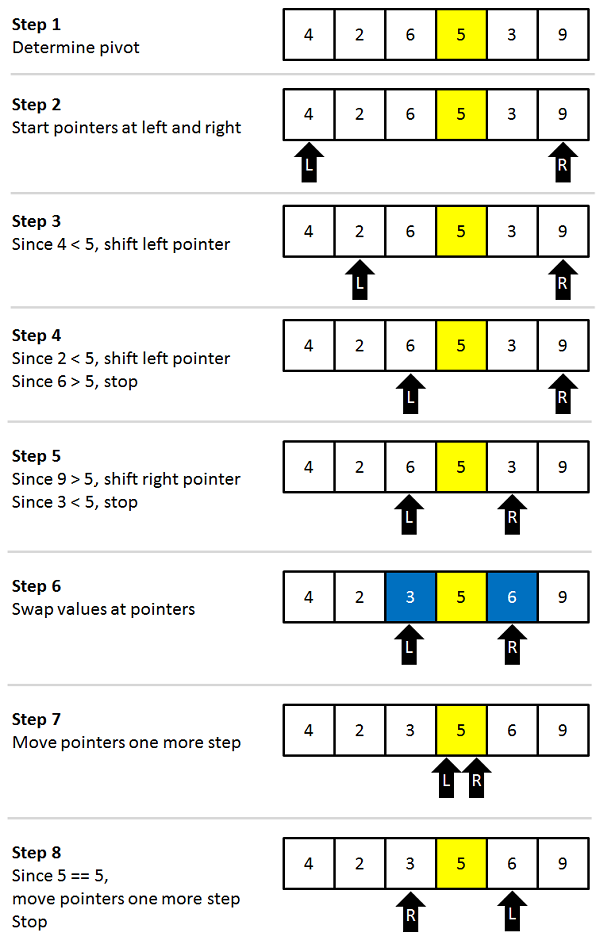
\includegraphics[scale=0.45]{pics/qsort1.png} \newline
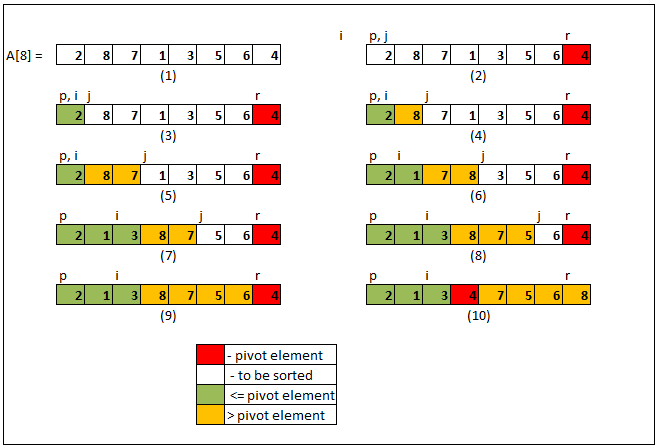
\includegraphics[scale=0.45]{pics/qsort2.png} \newline
\item Quick sort need random access ability.  

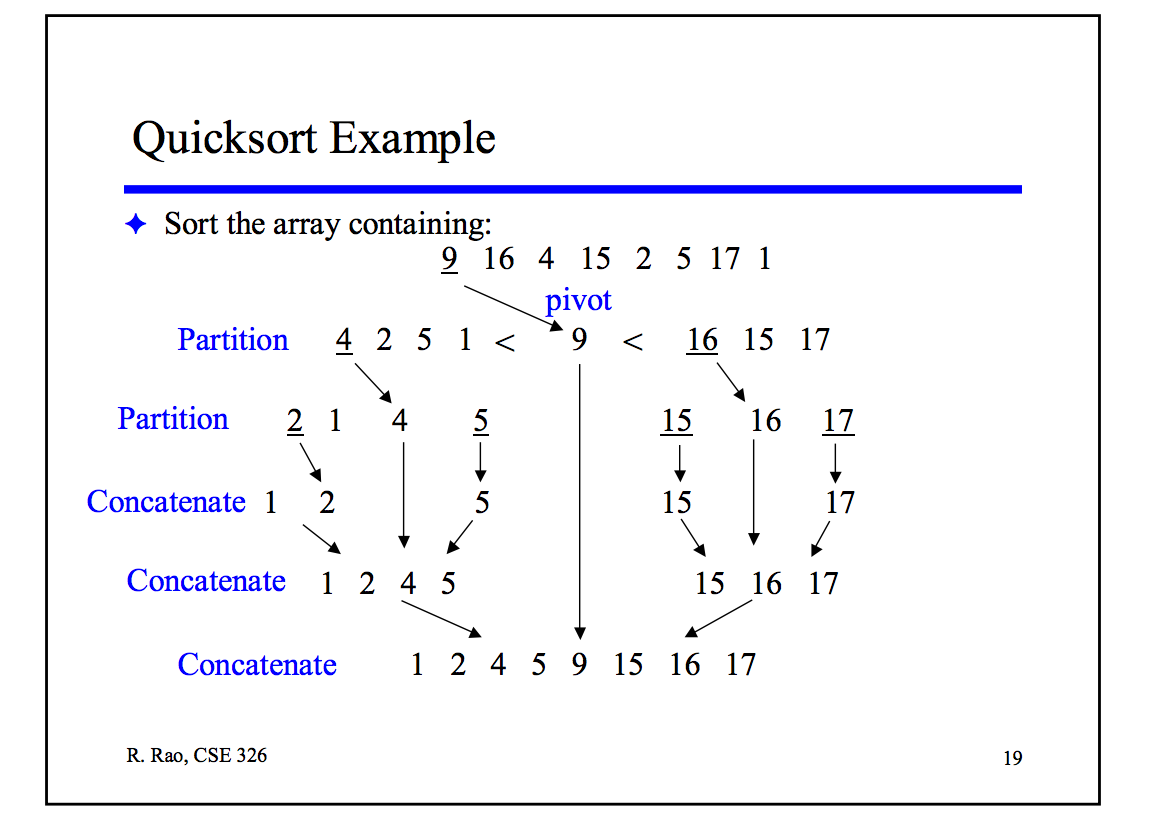
\includegraphics[scale=0.45]{pics/quick_sort.png} \newline


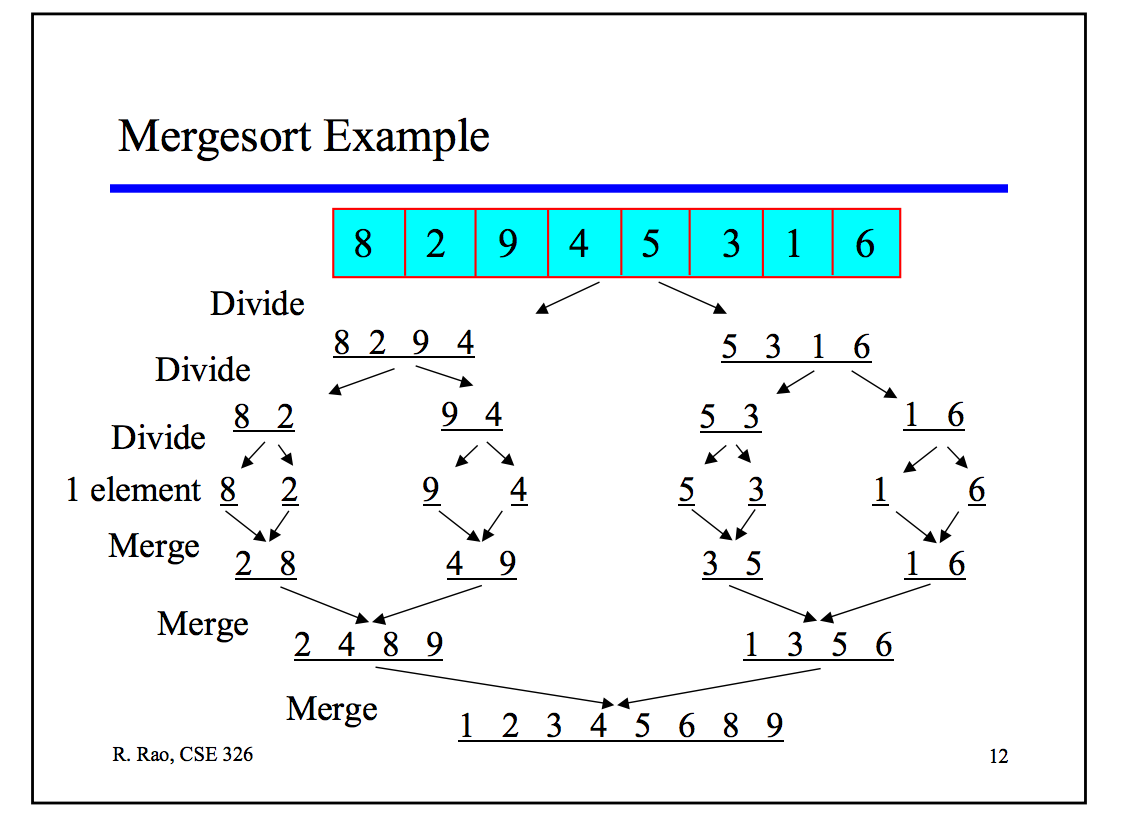
\includegraphics[scale=0.45]{pics/merge_sort.png} \newline



\end{itemize}

\subsection{introsort}
\begin{itemize}
	\item This is the method used in STL.
	
\begin{lstlisting}[frame=single, language=c++]
// A Utility function to perform intro sort
void IntrosortUtil(int arr[], int * begin,
int * end, int depthLimit)
{
	// Count the number of elements
	int size = end - begin;
	
	// If partition size is low then do insertion sort
	if (size < 16)
	{
		InsertionSort(arr, begin, end);
		return;
	}
	
	// If the depth is zero use heapsort
	if (depthLimit == 0)
	{
		make_heap(begin, end+1);
		sort_heap(begin, end+1);
		return;
	}
	
	// Else use a median-of-three concept to
	// find a good pivot
	int * pivot = MedianOfThree(begin, begin+size/2, end);
	
	// Swap the values pointed by the two pointers
	swapValue(pivot, end);
	
	// Perform Quick Sort
	int * partitionPoint = Partition(arr, begin-arr, end-arr);
	IntrosortUtil(arr, begin, partitionPoint-1, depthLimit - 1);
	IntrosortUtil(arr, partitionPoint + 1, end, depthLimit - 1);
	
	return;
}	
\end{lstlisting}

\end{itemize}

\subsection{Bucket and radix sort}
\begin{itemize}


\item Bucket sort is not comparison algorithm.  
\item we must know the maximum value in the unsorted array
\item How many objects in the unsorted array
\item If maximum value is not big, and objects is a lot. such as all student score (<100) in a school(1000). At this time, we can use Bucket sort. 
	
\item Firstly, we must know how to handle duplicates. Secondly,  Thirdly, we must have enough memory. If you sort telephone which will not allow duplicated value, you can build an bit array. And set bit 1 if there are number exist. It will save a lot of memories.   For duplicate, you can store a link in each bucket. (array item)

\item Radix sort is cousin of Bucksort BucketSort is more efficient for 'Dense' arrays, while RadixSort can handle sparse (well, not exactly sparse, but spaced-out) arrays well. Use \% operator to get radix each digit. 

\item $ 1\sim n^c-1$. $ 1\sim10^3-1 $  You can use 10 as radix, and sort it 3 times. 

\end{itemize}


\section{Greedy}
\begin{itemize} 

\item idea of Greedy
\begin{enumerate}
\item Solve a problem by making a sequence of decisions.

\item Decisions are made one by one in some order.

\item Each decision is made using a greedy criterion. At each stage we make a decision that appears to be the best at the time.

\item A decision, once made, is (usually) not changed later. 
\end{enumerate}


\item	You need a \textbf{greedy criterion} to make a local decision.
\item 	Examples: makin change, 0/1 knappack,  activity selection (largest subset) sorted according to their finishing time, topological orders.  Dijkstra, Kruskal, prim and sollin

\item Applications: Container Loading, 0/1 knapsack problem, Topological sorting, Bipartite cover, Single-source shortest paths, Minimum-cost spanning trees. 

\end{itemize}

\subsubsection{intervals questions}
\begin{itemize}
	\item \textbf{two basic tricks, sort, then do something when it overlap}.
	
	\item Meeting room question. 
	\begin{enumerate}
		\item minimum empty time. That is 0/1 knapback problem.
		\item two group collision intervals.
	\end{enumerate}
	

	\item overlap. (three questions)
\begin{enumerate}
	\item Non-overlap number. one meeting room, maximum meeting number. sort by end time, delete(ignore) if overlap. 
\begin{lstlisting}
	public int intervalSchedule(int[][] intvs) {
		if (intvs.length == 0) return 0;
		// sort
		Arrays.sort(intvs, new Comparator<int[]>() {
			public int compare(int[] a, int[] b) {
				return a[1] - b[1];
			}
		});
		
		int count = 1;
		int x_end = intvs[0][1];
		for (int[] interval : intvs) {
			int start = interval[0];
			if (start >= x_end) {
				// find next non-overlap interval, 
				//update x_end. 
				count++;
				x_end = interval[1];
			}
		}
		return count;
	}
\end{lstlisting}
	
	\item maximum overlap number. minimum meeting room numbers. sort by start time. you can use scan line. 
	
	\item merge overlap. sort by left. if overlap, then update right point; if non-overlap, find a new current intervals. 
\begin{lstlisting}
def merge(intervals):
if not intervals: return []
# 按区间的 start 升序排列
	intervals.sort(key=lambda intv: intv[0])
	res = []
	res.append(intervals[0])

	for i in range(1, len(intervals)):
		curr = intervals[i]
		# res 中最后一个元素的引用
		last = res[-1]
		if curr[0] <= last[1]:
			# 找到最大的 end
			last[1] = max(last[1], curr[1])
		else:
			# 处理下一个待合并区间
			res.append(curr)
	return res
\end{lstlisting}

\end{enumerate}
	
	\item interval cover. (two questions)
\begin{enumerate}
		
	\item minimum cover
\begin{lstlisting}
int videoStitching(int[][] clips, int T) {
	if (T == 0) return 0;
	// 按起点升序排列,起点相同的降序排列
	Arrays.sort(clips, (a, b) -> {
		if (a[0] == b[0]) {
			return b[1] - a[1];
		}
		return a[0] - b[0];
	});
	// 记录选择的短视频个数
	int res = 0;
	
	int curEnd = 0, nextEnd = 0;
	int i = 0, n = clips.length;
	while (i < n && clips[i][0] <= curEnd) {
		// 在第 res 个视频的区间内贪心选择下一个视频
		while (i < n && clips[i][0] <= curEnd) {
			nextEnd = Math.max(nextEnd, clips[i][1]);
			i++;
		}
		// 找到下一个视频,更新 curEnd
		res++;
		curEnd = nextEnd;
		if (curEnd >= T) {
			// 已经可以拼出区间 [0, T]
			return res;
		}
	}
	// 无法连续拼出区间 [0, T]
	return -1;
}	
\end{lstlisting}

	\item erase cover. Once find overlap, update right,  find non-overlap, update left and right. 
	\begin{lstlisting}
		int removeCoveredIntervals(int[][] intvs) {
			// 按照起点升序排列,起点相同时降序排列
			Arrays.sort(intvs, (a, b) -> {
				if (a[0] == b[0]) {
					return b[1] - a[1];
				}
				return a[0] - b[0]; 
			});
			
			// 记录合并区间的起点和终点
			int left = intvs[0][0];
			int right = intvs[0][1];
			
			int res = 0;
			for (int i = 1; i < intvs.length; i++) {
				int[] intv = intvs[i];
				// 情况一,找到覆盖区间
				if (left <= intv[0] && right >= intv[1]) {
					res++;
				}
				// 情况二,找到相交区间,合并
				if (right >= intv[0] && right <= intv[1]) {
					right = intv[1];
				}
				// 情况三,完全不相交,更新起点和终点
				if (right < intv[0]) {
					left = intv[0];
					right = intv[1];
				}
			}
			
			return intvs.length - res;
		}
	\end{lstlisting} 
	
\end{enumerate}	
	
\end{itemize}

\subsection{application}
\begin{itemize}
\item  Machine Scheduling, \textbf{sort all task according to start time, and minheap of machine end time. }

\item Container Loading and 0/1 knapsack problem are different. For 0/1 knapsack problem, we consider the value and weight together,  For greed algorithm, it change time complexity from $2^{n}$to $n.log(n)$, but 583/600 is withing 10\%, so it's very practical algorithm.  Don't underestimate it. 

\item Topological sorting: 
\begin{verbatim}
1) Select any one among vertices having no incoming edge
2) Put the node into the solution &  Remove the node and its outgoing edges from the graph
4) Repeat the above steps until no nodes remain

You need to InDegree[n] array to save and update all the vetex InDegree, and stack to store all the vetex which indegree is 0.  
\end{verbatim}


\item Bipartite-cover problems are NP-hard
\begin{verbatim}
A greedy method to develop a fast heuristic
Construct the cover A’ in stages
Select a vertex of A  using the greedy criterion:
Select a vertex of A that covers the largest # of uncovered vertices of B
\end{verbatim}

\item Dijkstra algorithm.  \newline
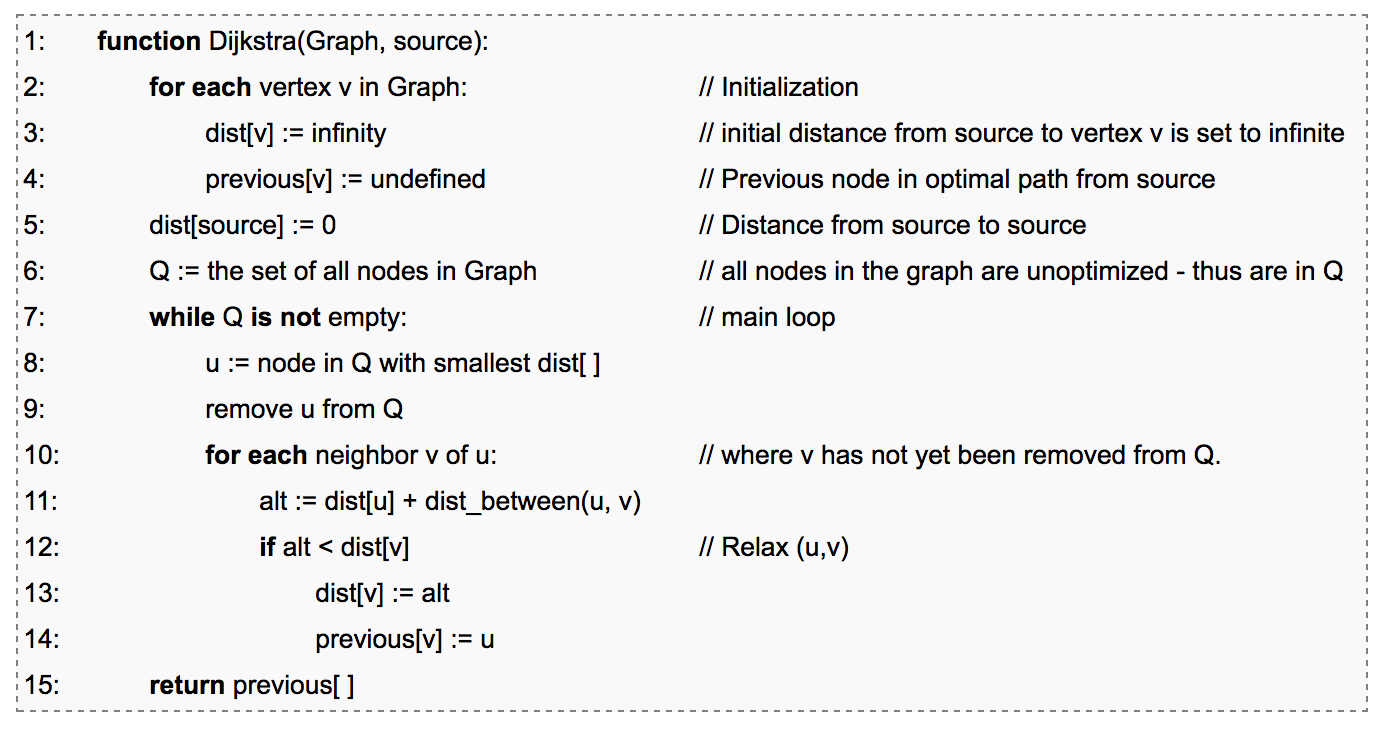
\includegraphics[scale=0.45]{pics/Dijkstra.png} \newline
\begin{enumerate}
\item The greedy idea lies in line 8
\item In line 8, it must shortest path to this vetex,  Because if it's not, There is shorter path, then, according to we select min in line 8, shorter one will be selected first, and this value HAS BEEN updated before. 
\item $O(n^{2})$
\item the shortest value is saved, it's also idea of dynamic programming.
\item Just like vertabi, you can think that they are the same. 
\end{enumerate}

\end{itemize}

\section{Divide Conquer}
\subsection{Binary search}
\begin{itemize}
	\item look for a certain number. 

\begin{lstlisting}[frame=single, language=c++]
int binarySearch(int arr[],int target, int i, int j) {
	int left = i;
	int right = j;
	while ( left<= right) {
		int mid = (left+right)/2;
		if (arr[mid] > target)
			right = mid - 1;
		else if (arr[mid] < target)
			left = mid + 1;
		else if (arr[mid] == target)
			return mid;
	}
	return -1;
} 
\end{lstlisting}

\begin{lstlisting}[frame=single, language=c++]
int left_bound(int arr[],int target, int i, int j) {
	int left = i;
	int right = j;
	while ( left<= right) {
		int mid = (left+right)/2;
		if (arr[mid] > target)
			right = mid - 1;
		else if (arr[mid] < target)
			left = mid + 1;
		else if (arr[mid] == target)
			right = mid-1;  //1) reduce to right in order to find left bound
	}
	
	if (left > j || arr[left] != target)
		return -1;  //3) in order to return left, left will go to the right boundary, 
	return left; //2) return left.   
}
\end{lstlisting}	


\begin{lstlisting}[frame=single, language=c++]
int right_bound(int arr[],int target, int i, int j) {
	int left = i;
	int right = j;
	while ( left<= right) {
		int mid = (left+right)/2;
		if (arr[mid] > target)
			right = mid - 1;
		else if (arr[mid] < target)
			left = mid + 1;
		else if (arr[mid] == target)
			left = mid+1;  //1) step left to find right bound
	}
	
	if (right < 0 || arr[right] != target)
		return -1;  //3) in order to return right, right will be too small
	return right; //2) return right.   
}	
\end{lstlisting}
	
\item Three methods summary are below:
\begin{enumerate}
	\item close left and right
	\item left bound reduce right, right bount add left;
	\item left bound return left, right bound return right.
	\item left may be too big, right maybe too small. 
	\item if no found, 
\begin{lstlisting}[frame=single, language=c++]
//if we want to find 4, then right point to 3, left point to 5
//when we quit while loop. 
//so left_bount return the 5 (smallest bigger than target),  
//right bount return 3( biggest smaller than target.)
right left
  3    5
\end{lstlisting}	


\begin{center}
		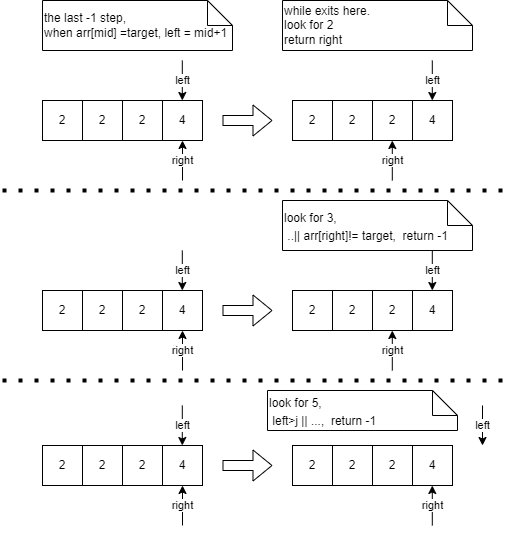
\includegraphics[width=0.7\linewidth]{pics/binary_search.drawio.png}
\end{center}

\end{enumerate}

\end{itemize}

\subsection{other }
\begin{itemize}
\item binary search:
\begin{enumerate}
\item only compare once, just  
\item avoid s+e overflow.
\item s will catch up e in the end, then break while loop 
\item check a[m] == k outside of while
\end{enumerate}

\begin{lstlisting}[frame=single, language=c++]
while(s<e) {
    //m=(s+e)/2;
    m = s/2+e/2 + s&e&1;
    if(a[m]<k)
        s = m+1;
    else 
       e = m;
}
if(a[m] == k) 
       return ture; 
\end{lstlisting}


\item An element in a sorted array can be found in O(log n) time via binary search. But suppose we rotate an ascending order sorted array at some pivot unknown to you beforehand. So for instance, 1 2 3 4 5 might become 3 4 5 1 2. Devise a way to find an element in the rotated array in O(log n) time.

The basic idea is DC(divided conquer.) 
\begin{enumerate}
	\item Use DC, The first part is end condition. For this question, the end atomic condition is e-b == 1(only two elements in it)
	\item If use array, better use index directly.
	\item When you have last atomic condition, you need to decide boundary  b, (e-b)/2, e. \textbf{When you decide boundary , you have to make half part of contents still includes answer. That is very useful hint for you to decide boundary value}
\end{enumerate}

\begin{lstlisting}[breaklines]
size_t find_rot(const vector<int> &vi, int b, int e){
	if (e-b ==1){
		return b;		
	}
	int pivot = b + (e-b)/2;
	cout<<"pivot"<<pivot<<endl;
	if (vi[b]<vi[pivot]){ 
		return find_rot(vi, pivot, e);
	}
	else{
		return find_rot(vi, b, pivot);
	}
}	
\end{lstlisting}
\begin{description}
	\item[label] \textbf{If you can divide it according certain condition, then you can use DC}
\end{description}

\end{itemize} 

\section{Dynamic programming}
\subsection{Basic Idea}
\begin{itemize}
	
\item \textbf{The basic question can be ask: can(bool), min or count(one number), all(list or vector)}
	
\item The difference between dynamic programming and greedy algorithms is that with dynamic programming, the subproblems overlap. That means that by "memoizing" solutions to some subproblems, you can solve other subproblems more quickly.   


\item The top-down approach is generally recursive (but less efficient) and more intuitive to implement as it is often a matter of recognizing the pattern in an algorithm and refactoring it as a dynamic programming solution.The bottom-up approach is generally iterative (and more efficient), but less intuitive and requires us to solve (and know!) the smaller problems first then use the combined values of the smaller problems for the larger solution.We refer to top-down solutions as memoization and bottom-up as tabulation.

\item Recursive: Simple, intuitive code
Unless care is taken to avoid recomputing previously computed values, the recursive program will have prohibitive complexity

\item Iterative: Not require additional space for the recursion stack
To minimize run time overheads, and hence to reduce actual run time, dynamic programming recurrences are almost always solved iteratively    (no recursion).

\item If we don’t need to solve all the problems and are just looking for the optimal solution, memorization is better.

If we do need to solve all the problems, that means we are going to make a lot of recursive calls, and tabulation is better.

The caveat is that memoization is generally more intuitive to implement especially when we don’t know the solution to subproblems, whereas tabulation requires us to know the solutions, or bottom, in advance, in order to build our way up.

\item In Divide and Conquer, the sub-problems are independent of each other while in case of Dynamic Programming, the sub-problems are not independent of each other (Solution of one sub-problem may be required to solve another sub-problem). Divide and Conquer works by dividing the problem into sub-problems, conquer each sub-problem recursively and combine these solutions. solves a problem by combining the solutions to  sub-problems

\begin{enumerate}
\item Partition the problem into non-overlapping sub-problems
\item Solve the sub-problems recursively
\item Combine their solutions to solve the original problem
\end{enumerate}


\item Dynamic Programming \\

Dynamic Programming is a technique for solving problems with overlapping subproblems. Each sub-problem is solved only once and the result of each sub-problem is stored in a table ( generally implemented as an array or a hash table) for future references. These sub-solutions may be used to obtain the original solution and the technique of storing the sub-problem solutions is known as memoization.

\item You may think of DP = recursion + re-use


\item The principle of optimality \\
No matter what the first decision, the remaining decisions must be optimal with respect to the state that results from this first decision
Dynamic programming may be used only when the principle of optimality holds. Useful when the sub-problems are overlapping

Solve an optimization problem by caching  sub-problem solutions rather than recomputing them

\begin{enumerate}
\item Verify that the principle of optimality holds  \newline
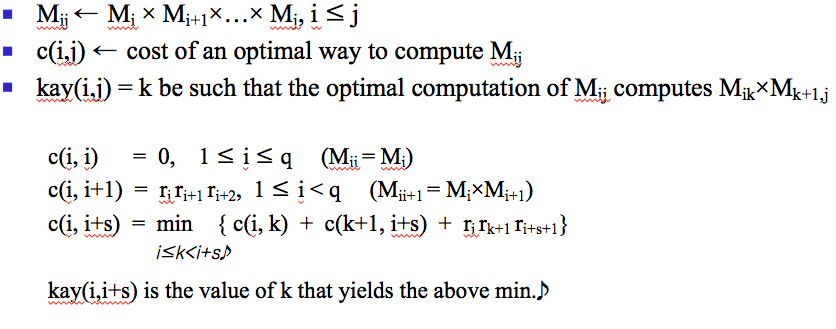
\includegraphics[scale=0.45]{pics/Recurrence.png} \newline

\item Set up the dynamic-programming recurrence equations
\item Solve the dynamic-programming recurrence equations for the value of the optimal solution
\item Perform a traceback step in which the solution itself is constructed
\end{enumerate}

\end{itemize}


\subsection{three questions}

\begin{itemize}
	
	\item The basic question can be ask: can(bool), min/max or count(one number), all(list or vector)
	

	\item  Write a function to return the minimum number of jumps to reach the end of the array (starting from the first element). Below is Min question
	
\begin{lstlisting}[numbers=none]
int arr[] = {1, 3, 5, 8, 9, 2, 6, 7, 6, 8, 9};

int minj(int arr[], int last){
	
	if (last ==1 && arr[last]>=1){
		return 1;
	}
	
	int min = last;
	for(int i = last-1; i>=0;i--){
		if (i+arr[i]>=last){
			int step = 1+minj(arr,i);
			if( step<min){
				min = step;
			}
		}    
	}
	return min;
}	
\end{lstlisting} 	
	
	
	\item below is getting all questions.  
\begin{lstlisting}[numbers=none]
int arr[] = {1, 3, 5, 8, 9, 2, 6, 7, 6, 8, 9};

vector<vector<int> >  minj(int arr[], int last){	
	if (last ==1 && arr[last]>=1){
		vector<int> v1 = {1};
		vector<vector<int> > v = {v1};
		return v;
	}	
	vector<vector<int> > result;
	
	int min = last;
	for(int i = last-1; i>=0;i--){
		if (i+arr[i]>=last){
			vector<vector<int> > result1 = minj(arr,i);
			for(auto e: result1){
				e.push_back(arr[i]);
				result.push_back(e);
			}
		}
	}
	return result;
}				
\end{lstlisting} 
	
	\item below is Can questions.  
\begin{lstlisting}[numbers=none]
int arr[] = {1, 3, 5, 8, 9, 2, 6, 7, 6, 8, 9};

bool  minj(int arr[], int last){
	
	if (last ==1 && arr[last]>=1){
		return true;
	}
	
	bool result = false;
	
	for(int i = last-1; i>=0;i--){
		if (i+arr[i]>=last){
			result = true && minj(arr,i);
			if(result)
				break;
		}
	}
	return result;
}	
\end{lstlisting} 

	\item Conclusion:
\begin{enumerate}
	\item can and min is little easy, min return one number, can return one bool. 
	\item all question need return a list, because each answer is a list, so here we return vector< vector >. 
	\item all question is suitable Top-bottom method. can and min is suitable for bottom-top method.
\end{enumerate}
		
\end{itemize}


\subsection{one dimension}
\begin{itemize}
	
	\item Longest Increasing Subsequence, top bottom method. There are a lot of overlap problem, so efficient is not good.

\begin{lstlisting}[numbers=none]
int _lis( int arr[], int n, int *max_ref)
{
	/* Base case */
	if (n == 1)
	return 1;
	
	// 'max_ending_here' is length of LIS ending with arr[n-1]
	int res, max_ending_here = 1;
	
	/* Recursively get all LIS ending with arr[0],
	arr[1] ... arr[n-2]. If arr[i-1] is smaller
	than arr[n-1], and max ending with arr[n-1]
	needs to be updated, then update it */
	for (int i = 1; i < n; i++){
		res = _lis(arr, i, max_ref);
		if (arr[i-1] < arr[n-1] && res + 1 > max_ending_here)
			max_ending_here = res + 1;
	}
	
	// Compare max_ending_here with the overall
	// max. And update the overall max if needed
	if (*max_ref < max_ending_here)
	*max_ref = max_ending_here;
	
	// Return length of LIS ending with arr[n-1]
	return max_ending_here;
}
\end{lstlisting}

	\item Longest Increasing Subsequence, bottom-top method. There are no overlap problem, so efficient is good

\begin{lstlisting}[numbers=none]
int lis( int arr[], int n ){
	int lis[n];
	lis[0] = 1;  
	
	/* Compute optimized LIS values in
	bottom up manner */
	for (int i = 1; i < n; i++ ){
		lis[i] = 1;
		for (int j = 0; j < i; j++ ) 
			if ( arr[i] > arr[j] && lis[i] < lis[j] + 1)
				lis[i] = lis[j] + 1;
	}
	
	// Return maximum value in lis[]
	return *max_element(lis, lis+n);
}
\end{lstlisting}


	\item house robber
\begin{lstlisting}[numbers=none]
	for (i ->n)
	for(j->i)
	max(dp[j]...)
\end{lstlisting}


	\item can target string be built by input string, top-bottom.

\begin{lstlisting}[numbers=none]
vector<string> input = {"ab", "abc", "cd", "def", "abcd", "ef" , "c"};
string target = "abcdef";

vector<vector<string> > ac(string target, const vector<string> & in ){
	if (target.size() == 0){
		return vector<vector<string>> {{}};
	}
	
	vector<vector<string>> last_result;
	
	for(auto i: input){
		if (target.find(i) == 0){
			string sub = target;
			sub.erase(0, i.size());
			vector<vector<string>> re = ac(sub, in);
			for(auto j : re){
				j.push_back(i);
				last_result.push_back(j);
			}
		}
	}
	return last_result;
}
\end{lstlisting} 

\item how many way can target string be built by input string, top-bottom.
\begin{lstlisting}[numbers=none]
vector<string> input = {"purp", "p", "ur", "le", "purpl"};
string target = "purple";

int ac(string target, const vector<string> & in ){	
	int arr[7] = {1, 0, 0, 0, 0, 0, 0};
	for(int i = 0;i<7;i++){
		for (auto s: input){
			int length = s.length();
			if(target.substr(i, length) == s)
			{
				arr[i+length] += arr[i];
			}		
		}
	}

	return arr[6];
}
\end{lstlisting} 

\end{itemize}

\subsubsection{conclusion}
\begin{itemize}
	\item For this problem, first, decide to use one dimension dp(lis array in previous example)
	\item dp definition(state) should be match with your questions, here, state is the length of LIS. 
	\item dp and recursive use the same state. For example, dp and return value of recursive are both length of LIS.
	\item A common template
	\begin{lstlisting}[numbers=none]
		for (i ->n)
		for(j->i)
		max(dp[j]...)
	\end{lstlisting}

\end{itemize}



\subsection{two dimension}

\begin{itemize}
\item The basic idea: \newline

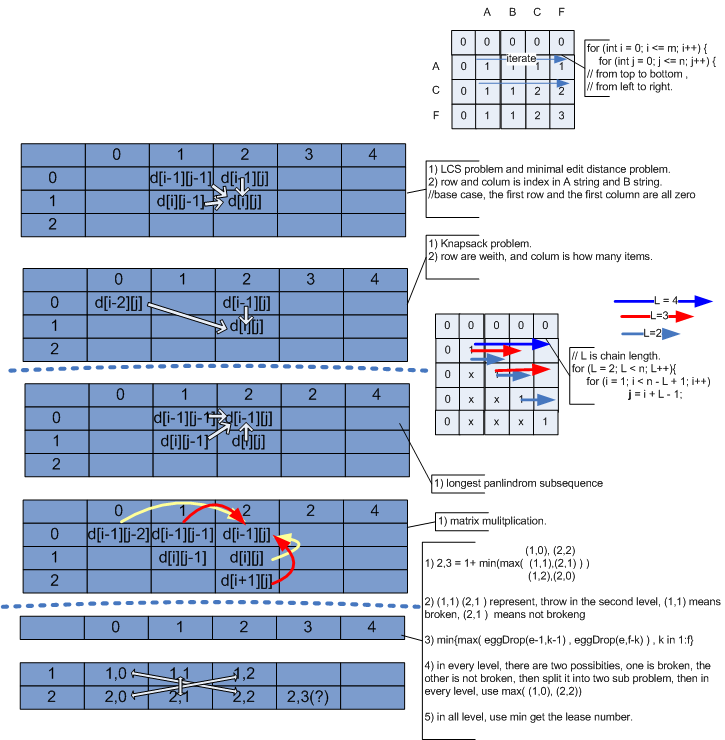
\includegraphics[scale=0.65]{pics/two_dimension.png} \newline

\item LCS problem 
\begin{lstlisting}[frame=single, language=c++]
/* Returns length of LCS for X[0..m-1], Y[0..n-1] */
int lcs( char *X, char *Y, int m, int n ) 
{ 
	int L[m + 1][n + 1]; 
	int i, j; 
	
	/* Following steps build L[m+1][n+1] in 
	bottom up fashion. Note that L[i][j] 
	contains length of LCS of X[0..i-1]
	and Y[0..j-1] */
	
	for (i = 0; i <= m; i++) { 
		for (j = 0; j <= n; j++) { 
			if (i == 0 || j == 0)  
				L[i][j] = 0;   
			//base case, the first row and the first column are all zero
			
			else if (X[i - 1] == Y[j - 1]) 
				L[i][j] = L[i - 1][j - 1] + 1; 
			
			else
			L[i][j] = max(L[i - 1][j], L[i][j - 1]); 
		} 
	} 
	
	/* L[m][n] contains length of LCS 
	for X[0..n-1] and Y[0..m-1] */
	
	return L[m][n]; 
} 	
\end{lstlisting}

\item minimal edit distance problem 
\begin{lstlisting}[frame=single, language=c++]
int min(int x, int y, int z) { return min(min(x, y), z); }
int editDistDP(string str1, string str2, int m, int n)
{
	// Create a table to store results of subproblems
	int dp[m + 1][n + 1];
	
	// Fill d[][] in bottom up manner
	for (int i = 0; i <= m; i++) {
		for (int j = 0; j <= n; j++) {
			// If first string is empty, only option is to
			// insert all characters of second string
			if (i == 0)
				dp[i][j] = j; // Min. operations = j
			
			// If second string is empty, only option is to
			// remove all characters of second string
			else if (j == 0)
				dp[i][j] = i; // Min. operations = i
			
			// If last characters are same, ignore last char
			// and recur for remaining string
			else if (str1[i - 1] == str2[j - 1])
				dp[i][j] = dp[i - 1][j - 1];
			
			// If the last character is different, consider
			// all possibilities and find the minimum
			else
				dp[i][j] = 1 + min(dp[i][j - 1], // Insert
						dp[i - 1][j], // Remove
					dp[i - 1][j - 1]); // Replace
		}
	}
	
	return dp[m][n];
}	
\end{lstlisting}

\item longest panlindrom subsequence (LPS)
\begin{lstlisting}[frame=single, language=c++]
// Returns the length of the longest palindromic subsequence in seq
int lps(char *str)
{
	int n = strlen(str);
	int i, j, cl;
	int L[n][n];  // Create a table to store results of subproblems
		
	// Strings of length 1 are palindrome of lentgh 1
	for (i = 0; i < n; i++)
	L[i][i] = 1;
	
	// Build the table. Note that the lower diagonal values of table are
	// useless and not filled in the process. The values are filled in a
	// manner similar to Matrix Chain Multiplication DP solution (See
	// https://www.geeksforgeeks.org/matrix-chain-multiplication-dp-8/). cl is length of
	// substring
	for (cl=2; cl<=n; cl++){
		for (i=0; i<n-cl+1; i++){
			j = i+cl-1;
			if (str[i] == str[j] && cl == 2)
				L[i][j] = 2;
			else if (str[i] == str[j])
				L[i][j] = L[i+1][j-1] + 2;
			else
				L[i][j] = max(L[i][j-1], L[i+1][j]);
		}
	}
	return L[0][n-1];
}

\end{lstlisting}


\item matrix multiply 
\begin{lstlisting}[frame=single, language=c++]
int MatrixChainOrder(int p[], int n)
{
	
	/* For simplicity of the program, one
	extra row and one extra column are
	allocated in m[][]. 0th row and 0th
	column of m[][] are not used */
	int m[n][n];
	
	int i, j, k, L, q;
	
	/* m[i, j] = Minimum number of scalar
	multiplications needed to compute the
	matrix A[i]A[i+1]...A[j] = A[i..j] where
	dimension of A[i] is p[i-1] x p[i] */
	
	// cost is zero when multiplying
	// one matrix.
	for (i = 1; i < n; i++)
	m[i][i] = 0;
	
	// L is chain length.
	for (L = 2; L < n; L++){
		for (i = 1; i < n - L + 1; i++){
			j = i + L - 1;
			m[i][j] = INT_MAX;
			for (k = i; k <= j - 1; k++){
				
				// q = cost/scalar multiplications
				q = m[i][k] + m[k + 1][j]
				+ p[i - 1] * p[k] * p[j];
				if (q < m[i][j])
				m[i][j] = q;
			}
		}
	}
	
	return m[1][n - 1];
}	
\end{lstlisting}

\item knapsack capacity
\begin{lstlisting}[frame=single, language=c++]
int knapSack(int W, int wt[], int val[], int n)
{
	int i, w;
	int K[n + 1][W + 1];
	
	// Build table K[][] in bottom up manner
	for(i = 0; i <= n; i++)
	{
		for(w = 0; w <= W; w++)
		{
			if (i == 0 || w == 0)
			K[i][w] = 0;
			else if (wt[i - 1] <= w)
			K[i][w] = max(val[i - 1] +
			K[i - 1][w - wt[i - 1]],
			K[i - 1][w]);
			else
			K[i][w] = K[i - 1][w];
		}
	}
	return K[n][W];
}	
\end{lstlisting}

\item egg drop
\begin{lstlisting}[frame=single, language=c++]
int eggDrop(int n, int k){
	/* A 2D table where entery
	eggFloor[i][j] will represent
	minimum number of trials needed for
	i eggs and j floors. */
	int eggFloor[n + 1][k + 1];
	int res;
	int i, j, x;
	
	// We need one trial for one floor and 0
	// trials for 0 floors
	for (i = 1; i <= n; i++) {
		eggFloor[i][1] = 1;
		eggFloor[i][0] = 0;
	}
	
	// We always need j trials for one egg
	// and j floors.
	for (j = 1; j <= k; j++)
	eggFloor[1][j] = j;
	
	// Fill rest of the entries in table using
	// optimal substructure property
	for (i = 2; i <= n; i++) {
		for (j = 2; j <= k; j++) {
			eggFloor[i][j] = INT_MAX;
			for (x = 1; x <= j; x++) {
				res = 1 + max(
				eggFloor[i - 1][x - 1],
				eggFloor[i][j - x]);
				if (res < eggFloor[i][j])
				eggFloor[i][j] = res;
			}
		}
	}
	
	// eggFloor[n][k] holds the result
	return eggFloor[n][k];
}
\end{lstlisting}



\end{itemize}



\section{backtracking}
\subsection{Basic}
\begin{itemize}
	
	\item The basic backtracking code
\begin{lstlisting}[frame=single, language=c++]
result = []
def backtrack(track, select_list):
	if end_condition:
		result.add( track)
		return

	for option in select_list:
		select one
		backtrack(track, select_list)
		revert the select	
\end{lstlisting}

\item below is DFS. There is two different: 1) In DFS, we don't need to records all the path, so just don't use track. 2) DFS need to check if unvisited. but most backtrack problem deal with multi-branch tree problem(such as permutation or eight queen problem), so usually we don't check if node is unvisited. The basic idea is the same. 
\begin{lstlisting}[frame=single, language=c++]
	DFS(current){
		visit current;
		for all(next to current){
			if(unvisited(next)){
				DFS(next);
			}
		}
	}
\end{lstlisting} 


	\item If we don't want to return all the result, but one, we can change it to 
\begin{lstlisting}[frame=single, language=c++]
result = []
bool backtrack(track, select_list):
	if end_condition:
		result.add(track)
		return true;
	
	for option in select_list:
		select one
		if(backtrack(track, select_list))
			return true;
		revert the select	
\end{lstlisting}
\begin{description}
	\item[Line9-10] This if will stop the recursive and return the true direct to the root.
\end{description}


\begin{lstlisting}
List<List<Integer>> res = new LinkedList<>();
 //remember recursive path
LinkedList<Integer> track = new LinkedList<>();

// main function
public List<List<Integer>> subsets(int[] nums) {
	backtrack(nums, 0);
	return res;
}


void backtrack(int[] nums, int start) {
	
	res.add(new LinkedList<>(track));
	
	// main frame
	for (int i = start; i < nums.length; i++) {
		// select
		track.addLast(nums[i]);
		//  use start to trim
		backtrack(nums, i + 1);
		// unselect
		track.removeLast();
	}
}


\end{lstlisting}


\subsection{permutation, combination and subset}
\subsubsection{no duplicate, single select}
\begin{itemize}
	\item Two important tree structures.
\begin{center}
	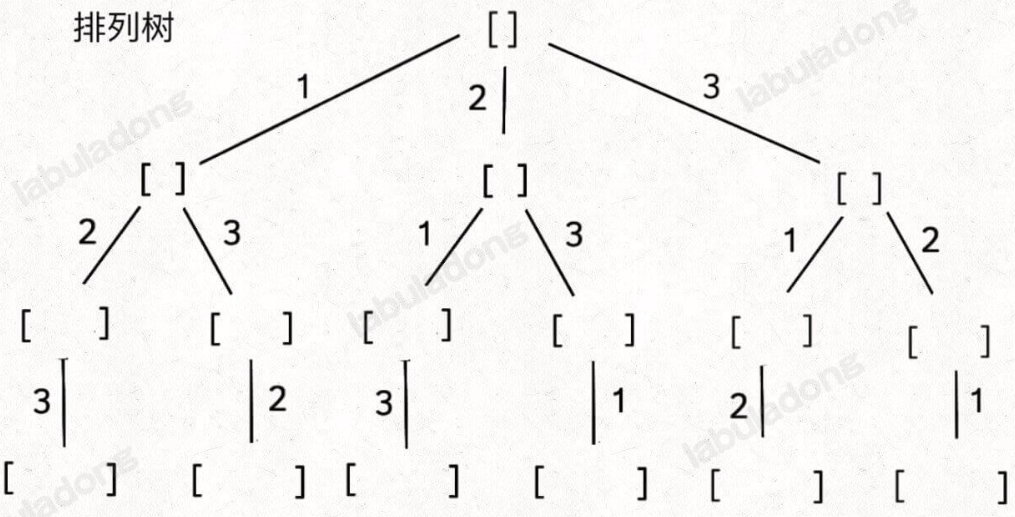
\includegraphics[width=0.7\linewidth]{pics/per}
	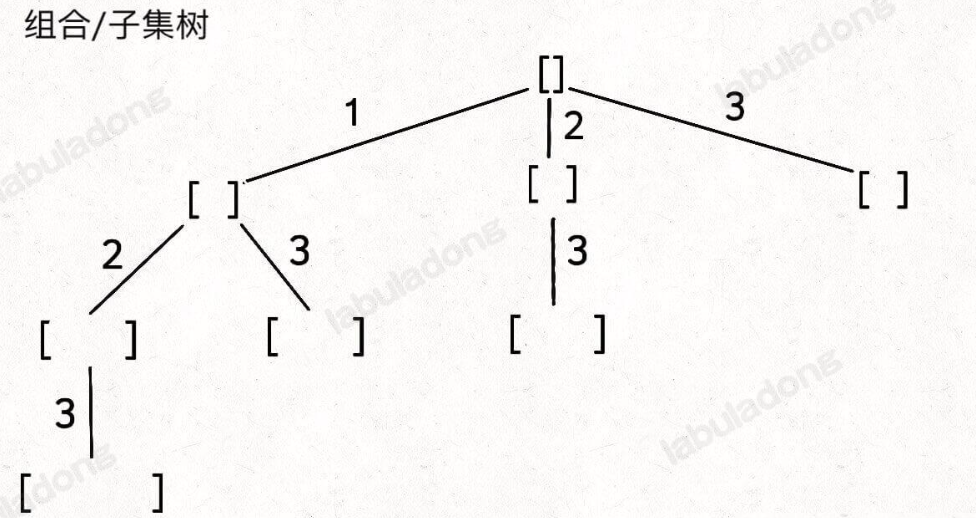
\includegraphics[width=0.7\linewidth]{pics/com}
\end{center}
		
	\item dombination can be seen as a child question of subset. 
	\begin{center}
		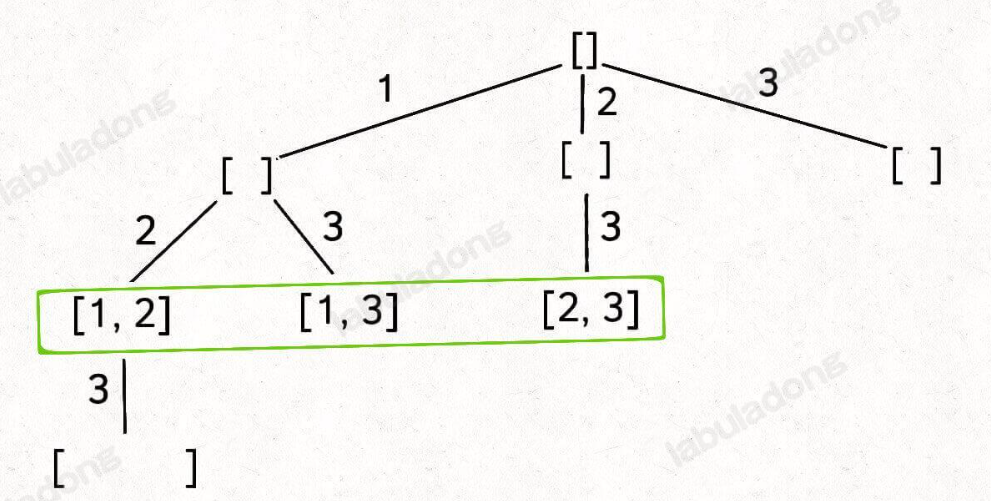
\includegraphics[width=0.7\linewidth]{pics/subset}
	\end{center}
	
\end{itemize}

	\item \textbf{subset problem}. 
\begin{enumerate}
	\item Each node(from current node to root,including root(empty set)) is an answer
	\item Don't need base case here.  when i>=len, for will return without any execution.
	\item Refer the combination tree figure to help to understand this code
\end{enumerate}
	
\begin{lstlisting}
void sub(int arr[], int len, int start, vector<int>& result) {
	cout << "one answer is ( ";
	for (int i = 0; i < result.size(); i++) {
		cout << result[i] << " ";
	}
	cout << ")" << endl;
	
	for (int i = start; i < len; ++i) {
		result.push_back(arr[i]);  
		sub(arr, len, i + 1, result);
		result.pop_back();
	}
}
sub(arr, 3, 0, result)
\end{lstlisting}
	
	\item \textbf{combination problem}, the same idea as subset, just add a parameter k. When one answer length is k, print it out. 
\begin{lstlisting}
void com(int arr[], int len, int start, int k, vector<int>& result){
	if (result.size() == k) {
		cout << "one answer is ( ";
		for (int i = 0; i < result.size(); i++) {
			cout << result[i] << " ";
		}
		cout << ")" << endl;
	}
	
	for (int i = start; i < len; ++i) {
		result.push_back(arr[i]);  
		com(arr, len, i + 1, k, result);
		result.pop_back();
	}
}	
\end{lstlisting}

	\item \textbf{permutation problem}. 
\begin{enumerate}
	\item Base case is size == len
	\item You must use used array here to remember which element you have used. 
\end{enumerate}
\begin{lstlisting}
void per(int arr[], int len, int used[], vector<int>& result) {
	if (result.size() == len) {
		cout << "one answer is ( ";
		for (int i = 0; i < result.size(); i++) {
			cout << result[i] << " ";
		}
		cout << ")" << endl;
	}
	for (int i = 0; i < len; ++i) {
		if (used[i] == 1)
		continue;
		result.push_back(arr[i]); 
		used[i] = 1;
		per(arr, len, used, result);
		result.pop_back();
		used[i] = 0;
	}
}	
\end{lstlisting}
	\item For permutation problem, there is another easy implementation. You don't need extra result vector, but you have to use swap. They use the same basic backtrack idea.
\begin{lstlisting}
//all permutation. here there is a trick, we don't need track, but the basic idea is the same. 
void permute(char a[], int i, int n){
	int j;
	if (i == n){  //end_condition, 
		cout << a << endl;
		return;
	}
	
	for (j = i; j <= n; j++){  // all options in select_list
		swap(a[i], a[j]);     //select one
		permute(a, i+1, n);
		swap(a[i], a[j]);    //revoke select.
	}
} 	

\end{lstlisting}

\end{itemize}

\subsubsection{no duplicate, multi select}
\begin{itemize}
	\item The basic idea is just like before, for combination, we use i+1 to call recursion implementation single select, if you can multi select, just use i here. In order to avoid dead loop, this questions need a target to end loop, A typical question is coin problem.
\begin{lstlisting}
void sub_multi_select(int arr[], int len, int start, vector<int>& result, int target) {
	auto sum = std::accumulate(result.begin(), result.end(), 0);
	if (sum > target)
	return;
	if (sum == target) {
		cout << "one answer is ( ";
		for (int i = 0; i < result.size(); i++) {
			cout << result[i] << " ";
		}
		cout << ")" << endl;
	}
	
	for (int i = start; i < len; ++i) {
		result.push_back(arr[i]);
		sub_multi_select(arr, len, i, result, target);  //Pay attention here, not pass i+1, but pass i. 
		result.pop_back();
	}
}

int arr[3] = { 1,2,5};
vector<int> result;
sub_multi_select(arr, 3, 0, result, 10);

one answer is ( 1 1 1 1 1 1 1 1 1 1 )
one answer is ( 1 1 1 1 1 1 1 1 2 )
one answer is ( 1 1 1 1 1 1 2 2 )
one answer is ( 1 1 1 1 1 5 )
one answer is ( 1 1 1 1 2 2 2 )
one answer is ( 1 1 1 2 5 )
one answer is ( 1 1 2 2 2 2 )
one answer is ( 1 2 2 5 )
one answer is ( 2 2 2 2 2 )
one answer is ( 5 5 )

\end{lstlisting}

\begin{center}
	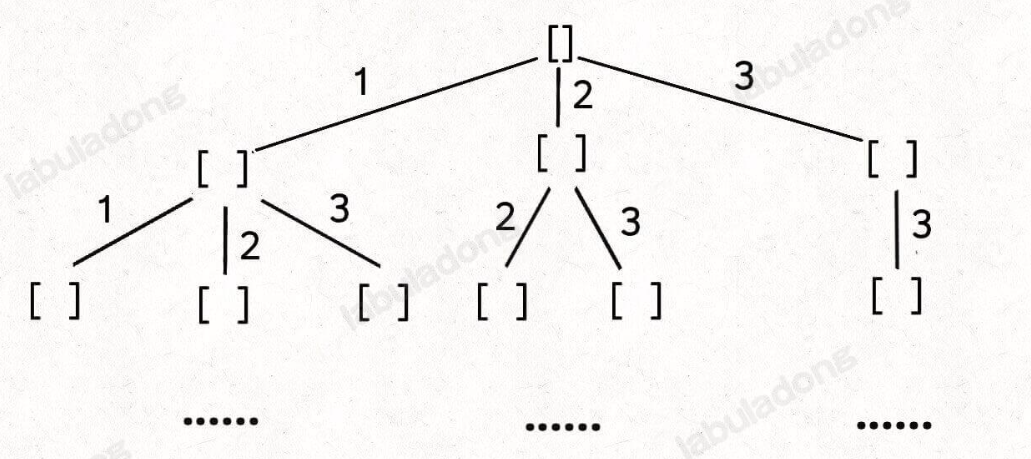
\includegraphics[width=0.7\linewidth]{pics/sub_multi}
\end{center}

	\item multi select permutation, Code is very easy, don't use used array. The time complexity is power(n, n). That is the only question which has so high time complexity. 
	

\end{itemize}

\subsubsection{duplicate, single select}
\begin{itemize}
	
	\item For combination, need to sort, then trim(prune) a branch which doesn't meet condition. For combination, first sort, then use a condition to trim
\begin{lstlisting}
	....
	for (int i = start; i < len; ++i) {
		if(i>start && arr[i] == arr[i-1]) // trimming happens in these two 
			continue;                     // statements, so we need to sort first. 
		result.push_back(arr[i]);  
		sub(arr, len, i + 1, result);
		result.pop_back();
	}	
	....
\end{lstlisting}

\begin{center}
	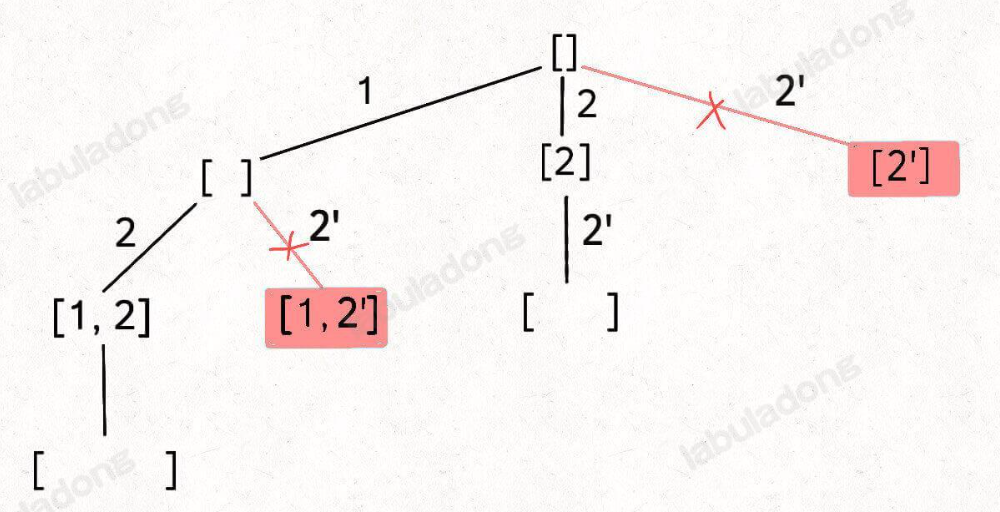
\includegraphics[width=0.7\linewidth]{pics/com_duplicate}
\end{center}
	

	\item For permutation, need to sort, then trim(prune) a branch which doesn't meet condition. 
\begin{lstlisting}
	....
	for (int i = start; i < len; ++i) {
		if(i>start && arr[i] == arr[i-1] && !used[i-1]) // trimming happens in these two 
			continue;                                // statements, so we need to sort first. 
		result.push_back(arr[i]);  
		sub(arr, len, i + 1, result);
		result.pop_back();
	}	
	....
\end{lstlisting}
	\item How to understand \verb|!used[i-1]|? 
	\begin{center}
		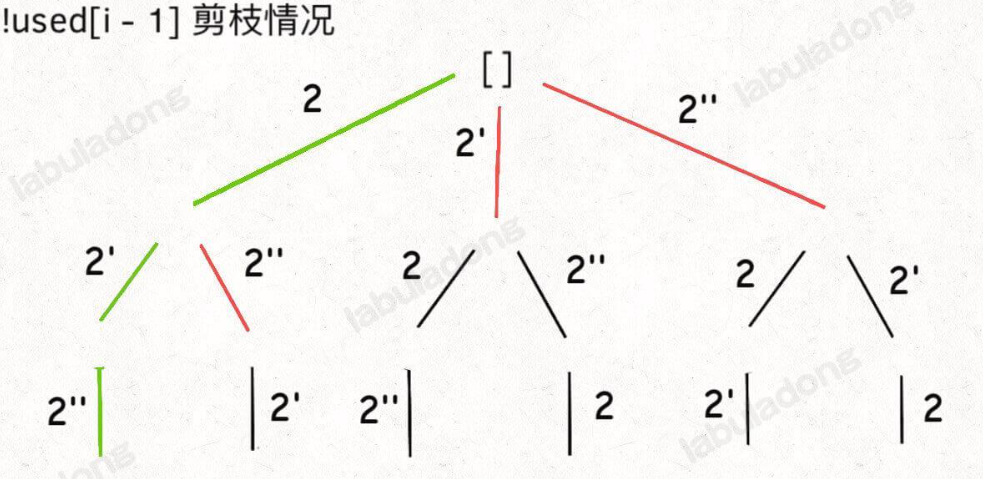
\includegraphics[width=0.7\linewidth]{pics/per_duplicate}
	\end{center}
	

\end{itemize}

\subsubsection{parenthesis}
\begin{itemize}
	\item The trimming idea can be applied in parenthesis problem, the basic problem is also permutation problem, but you need to trimming the branch. 
	anytime, left parenthesis should be greater or equal right parenthesis. 
\begin{lstlisting}

vector<string> generateParenthesis(int n) {
	vector<string> res;  //all results
	
	string track;
	// left and right parenthesis number are both n
	backtrack(n, n, track, res);
	return res;
}


void backtrack(int left, int right, 
string& track, vector<string>& res) {
	//left is less right, illegal.
	if (right < left) return;
	
	if (left < 0 || right < 0) return;
	// all is 0, get a legal result.
	if (left == 0 && right == 0) {
		res.push_back(track);
		return;
	}
	
	// try to put a left 
	track.push_back('('); 
	backtrack(left - 1, right, track, res);
	track.pop_back(); 
	
	// try to put a right.
	track.push_back(')'); 
	backtrack(left, right - 1, track, res);
	track.pop_back(); 
}
\end{lstlisting}
\end{itemize}

\subsubsection{summary}
\begin{itemize}
	
	\item four code compare: They are the most common used code template for back trace, you need to understand and 
\begin{enumerate}
	\item code 1: multi tree, call  call backtrace(i),  backtrace(i-1), backtrace(i-2)... //This will cause a multi branch tree, and the first level has n branches, 
	//The second level has n-1 branches, untill the last level has only 1 branches.   O(n*n)
\begin{lstlisting}
	for(i ..n )
	backtrace( i+1)
\end{lstlisting}
	
	\begin{center}
		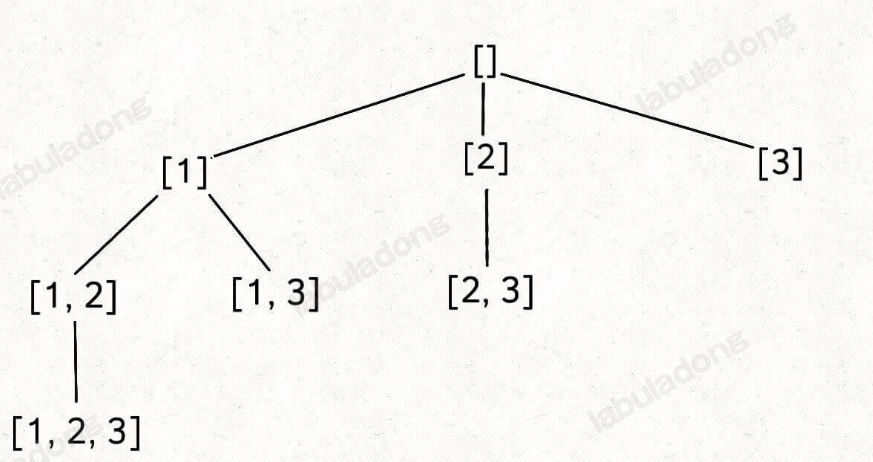
\includegraphics[width=0.7\linewidth]{pics/sub}
	\end{center}
	
	\item code 2: multi tree, on each level,  i, i-1,  i-2 backtrace O(n!)
\begin{lstlisting}
	for(j = i ..n )  // on i level, each backtrace trun (n-i) times. 
		backtrace( i+1)
\end{lstlisting}

	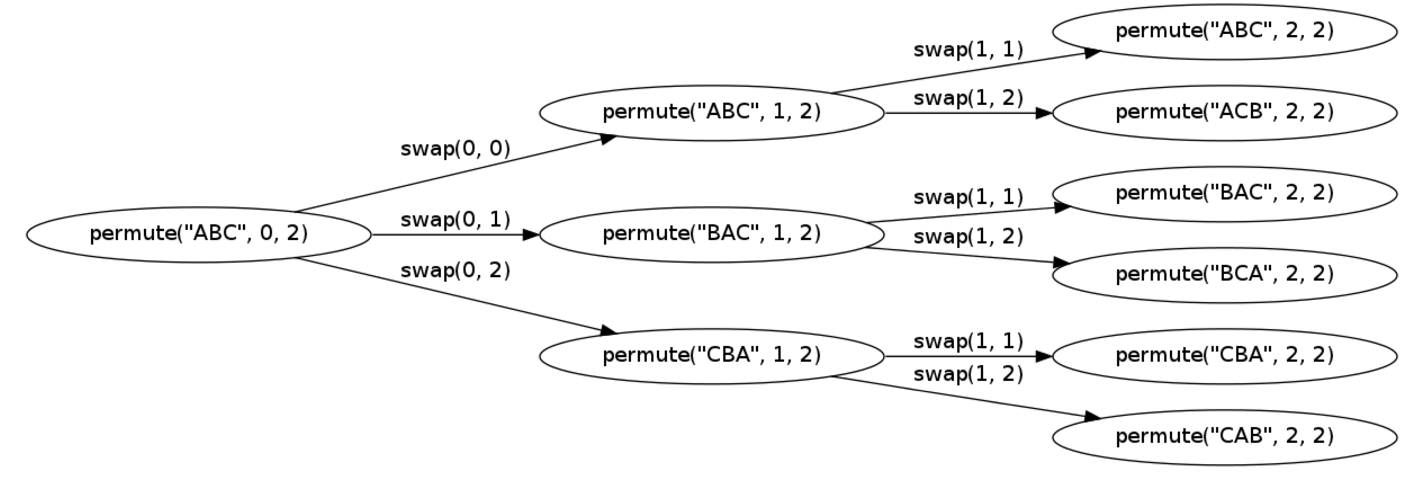
\includegraphics[scale=0.25]{pics/permutation.png}

	\item code 3: binary tree, global result, need reverse
	
	\item code 4: binary tree, stack partial result, don't need reverse. global result.
\end{enumerate}

\end{itemize}


\section{branch and bound}
\begin{itemize}
\item Backtracking:
\begin{enumerate}
\item It is used to find all possible solutions available to the problem.
\item It traverse tree by DFS(Depth First Search).
\item It realizes that it has made a bad choice \& undoes the last choice by backing up.
\item It search the state space tree until it found a solution.
\item It involves feasibility function.
\end{enumerate}


\item Branch-and-Bound
\begin{enumerate}
\item It is used to solve optimization problem.
\item It may traverse the tree in any manner, DFS or BFS.
\item It realizes that it already has a better optimal solution that the pre-solution leads to so it abandons that pre-solution.
\item It completely searches the state space tree to get optimal solution.
\item It involves bounding function.

\item Searches a solution space that is often organized as a tree (like backtracking)
\item Usually searches a tree in a breadth-first / least-cost manner (unlike backtracking)

\end{enumerate}

\item Difference between DFS and backtracking is:
\begin{enumerate}
\item Backtracking is a more general purpose algorithm. Depth-First search is a specific form of backtracking related to searching tree or graphic structures.  
\item For a problem, answer space can be described as a tree graphic structure, such as 0/1 backpack problem. at this time, backtracking use DFS to search the answer space, and use questions related condition to prune the sub-tree and com back. So in this way, you can think backtracking = DFS+prune. 

\item For mouse raze, because, prune is "no next neighbor", just like DFS, so DFS and backtracking are the totally same.
\end{enumerate}

\item Difference between branch-bound  and backtracking is about size
\begin{enumerate}
\item backtracking use stack and only add one child each time, so it use less memory compared with branch-bound
\item branch-bound store all possible child in queue, so if answer is near root, it will find answer quickly. 

\item win in size, but lose in time. backtracking will 1) find answer slowly, 2) branch-bound will find optimal answer. 
\end{enumerate}

\item dp and bound code for 0-1 back pack.  dp only can deal with integral weight. but bound can deal with float value. This code can run and print out all the value, it can help you to understand the idea behind these two important algorithms. 

\begin{lstlisting}
// C++ program to solve knapsack problem using
// branch and bound
#include <algorithm>
#include <queue>
#include <stack>
#include <iostream>
using namespace std;

// Structure for Item which store weight and corresponding
// value of Item
struct Item
{
	float weight;
	int value;
};

// Node structure to store information of decision
// tree
struct Node
{
	// level  --> Level of node in decision tree (or index
	//             in arr[]
	// profit --> Profit of nodes on path from root to this
	//            node (including this node)
	// bound ---> Upper bound of maximum profit in subtree
	//            of this node/
	int level, profit, bound;
	float weight;
};

// Comparison function to sort Item according to
// val/weight ratio
bool cmp(Item a, Item b)
{
	double r1 = (double)a.value / a.weight;
	double r2 = (double)b.value / b.weight;
	return r1 > r2;
}

// Returns bound of profit in subtree rooted with u.
// This function mainly uses Greedy solution to find
// an upper bound on maximum profit.
int bound(Node u, int n, int W, Item arr[])
{
	// if weight overcomes the knapsack capacity, return
	// 0 as expected bound
	if (u.weight >= W)
	return 0;
	
	// initialize bound on profit by current profit
	int profit_bound = u.profit;
	
	// start including items from index 1 more to current
	// item index
	int j = u.level + 1;
	int totweight = u.weight;
	
	// checking index condition and knapsack capacity
	// condition
	while ((j < n) && (totweight + arr[j].weight <= W))
	{
		totweight += arr[j].weight;
		profit_bound += arr[j].value;
		j++;
	}
	
	// If k is not n, include last item partially for
	// upper bound on profit
	if (j < n)
	profit_bound += (W - totweight) * arr[j].value /
	arr[j].weight;
	
	return profit_bound;
}

// Returns maximum profit we can get with capacity W
int knapsack(int W, Item arr[], int n)
{
	// sorting Item on basis of value per unit
	// weight.
	sort(arr, arr + n, cmp);
	
	// make a queue for traversing the node
	queue<Node> Q;
	Node u, v;
	
	// dummy node at starting
	u.level = -1;
	u.profit = u.weight = 0;
	Q.push(u);
	
	// One by one extract an item from decision tree
	// compute profit of all children of extracted item
	// and keep saving maxProfit
	int maxProfit = 0;
	while (!Q.empty())
	{
		// Dequeue a node
		u = Q.front();
		Q.pop();
		
		// If it is starting node, assign level 0
		if (u.level == -1)
		v.level = 0;
		
		// If there is nothing on next level
		if (u.level == n - 1)
		continue;
		
		// Else if not last node, then increment level,
		// and compute profit of children nodes.
		v.level = u.level + 1;
		
		// Taking current level's item add current
		// level's weight and value to node u's
		// weight and value
		v.weight = u.weight + arr[v.level].weight;
		v.profit = u.profit + arr[v.level].value;
		
		// If cumulated weight is less than W and
		// profit is greater than previous profit,
		// update maxprofit
		if (v.weight <= W && v.profit > maxProfit)
		maxProfit = v.profit;
		
		// Get the upper bound on profit to decide
		// whether to add v to Q or not.
		v.bound = bound(v, n, W, arr);
		cout << "look here" << v.weight << " " << v.bound <<" "<<maxProfit<<endl;
		
		// If bound value is greater than profit,
		// then only push into queue for further
		// consideration
		if (v.bound > maxProfit)
		Q.push(v);
		
		// Do the same thing,  but Without taking
		// the item in knapsack
		v.weight = u.weight;
		v.profit = u.profit;
		v.bound = bound(v, n, W, arr);
		if (v.bound > maxProfit)
		Q.push(v);
	}
	
	return maxProfit;
}

// driver program to test above function
int knapsack_back(int W, Item arr[], int n)
{
	// sorting Item on basis of value per unit
	// weight.
	sort(arr, arr + n, cmp);
	
	// make a queue for traversing the node
	stack<Node> S;
	Node u, v;
	
	// dummy node at starting
	u.level = -1;
	u.profit = u.weight = 0;
	S.push(u);
	
	// One by one extract an item from decision tree
	// compute profit of all children of extracted item
	// and keep saving maxProfit
	int maxProfit = 0;
	while (!S.empty())
	{
		// Dequeue a node
		u = S.top();
		S.pop();
		
		// If it is starting node, assign level 0
		if (u.level == -1)
		v.level = 0;
		
		// If there is nothing on next level
		if (u.level == n - 1)
		continue;
		
		// Else if not last node, then increment level,
		// and compute profit of children nodes.
		v.level = u.level + 1;
		
		
		// Do the same thing,  but Without taking
		// the item in knapsack
		v.weight = u.weight;
		v.profit = u.profit;
		S.push(v);
		
		
		// Taking current level's item add current
		// level's weight and value to node u's
		// weight and value
		v.weight = u.weight + arr[v.level].weight;
		v.profit = u.profit + arr[v.level].value;
		
		// If cumulated weight is less than W and
		// profit is greater than previous profit,
		// update maxprofit
		if (v.weight <= W && v.profit > maxProfit)
		maxProfit = v.profit;
		
		
		// If bound value is greater than profit,
		// then only push into queue for further
		// consideration
		
		S.push(v);
		
		
	}
	
	return maxProfit;
}


int knapsack_dp() {
	// base case 
	//{2, 40}, { 3.14, 50 }, { 1.98, 100 }, { 5, 95 }, { 3, 30 }
	int W = 10;
	int N = 5;
	int val[] = {40, 50, 100, 95, 30};
	int wt[] = { 2, 4, 2, 5, 3 };
	int dp[6][11];
	for (int i = 0; i <= N; i++) {
		for (int w = 0; w <= W; w++) {
			if (i == 0)
			dp[i][w] = 0;
			if (w == 0)
			dp[i][w] = 0;
		}
	}
	for (int i = 1; i <= N; i++) {
		for (int w = 1; w <= W; w++) {
			if (w - wt[i - 1] < 0) {
				
				dp[i][w] = dp[i - 1][w];
			}
			else {
				
				dp[i][w] = max(
				dp[i - 1][w - wt[i - 1]] + val[i - 1],
				dp[i - 1][w]
				);
			}
		}
	}
	
	for (int i = 1; i <= N; i++) {
		for (int w = 1; w <= W; w++) {
			cout << dp[i][w] << " ";
		}
		cout << endl;
	}
	
	return dp[N][W];
}


int main()
{
	int W = 10;   // Weight of knapsack
	Item arr[] = { {2, 40}, {3.14, 50}, {1.98, 100},
		{5, 95}, {3, 30} };
	int n = sizeof(arr) / sizeof(arr[0]);
	
	cout << "Maximum possible profit = "
	<< knapsack(W, arr, n) << endl;
	
	//dp 
	knapsack_dp();
	
	//back track
	cout<<"back track"<< knapsack_back(W, arr, n) << endl;	
	return 0;
}
\end{lstlisting}


\item eight queen
\begin{lstlisting}
	vector<vector<string>> res;
	vector<vector<string>> solveNQueens(int n) {
		
		// '.' is  void, 'Q' is queen
		vector<string> board(n, string(n, '.'));
		backtrack(board, 0);
		return res;
	}
	
	
	void backtrack(vector<string>& board, int row) {
		// base case
		if (row == board.size()) {
			res.push_back(board);
			return;
		}
		
		int n = board[row].size();
		for (int col = 0; col < n; col++) {
			// exclude
			if (!isValid(board, row, col)) {
				continue;
			}
			// make decision
			board[row][col] = 'Q';
			// go deeper
			backtrack(board, row + 1);
			// reverse
			board[row][col] = '.';
		}
	}
\end{lstlisting}

\item recursive 0-1 pack pack. \textbf{this is back trace, but why don't we have reverse decision? because in eight queen, we use reference parameter pass it to function(all function share). Here, we use stack, in each level, we have saved the local variable( you can think that it has been reversed by poping stack.) } That is the difference.  Another important thing is that for 0-1 pack and eight queen,  we need a logically recursive tree. So we need to simulate a "level" conception.  \textbf{0-1 pack stack solution, we save level information to the each node. 0-1 recursive solution, we use int i (array index)as level information. in eight queen, we use row information as level information }. level is the level information in the recursive solution tree.  
\begin{lstlisting}
public int maxW = Integer.MIN_VALUE; 
// cw current weight, i: current item
// call with f(0, 0, a, 10, 100)
public void f(int i, int cw, int[] items, int n, int w) {
	if (cw == w || i == n) { // cw==w is full or select all items
		if (cw > maxW) maxW = cw;
		return;
	}
	f(i+1, cw, items, n, w);
	if (cw + items[i] <= w) {// bigger than w, give up
		f(i+1,cw + items[i], items, n, w);
	}
}
2.
\end{lstlisting}


\item A example can be see in ref PPT.  container and ship problems. 

\end{itemize}

\section{code template}
\begin{enumerate}
	\item binary search
	\item BFS
	\item DFS
	\item slide windows
	\item DP
\end{enumerate}


\chapter{Summary}
\section{array and link}
\begin{itemize}
	\item %右面最大差, leader, 等数组问题, 需要保持一个min, or max, 从左面或右面扫描
	\item mono stack
	\item mono queue. 
	\item %三个链表问题, delete current node, 只需要删除后面一个temp, middle point, (fast && fast->next不是空); reverse lisk, trail, middle, lead 三个指针。
	
	\item %circular queue,里面是一个数组, front指向空, front==rear is empty, (rear+1)\%length == front 是满。基于这些,就可以写出push and pop 了。 
	
	\item heap (child-1)/2 is parent.  Parent*2+1 is left child, parent*2+2 is right child.
\end{itemize}
\section{dp}
\begin{itemize}
	\item %动态规划问题的一般形式就是求最值。 既然是要求最值,核心问题是什么呢?求解动态规划的核心问题是穷举。 明确 base case -> 明确「状态」-> 明确「选择」 -> 定义 dp 数组/函数的含义。 我把这部分理论总结为“一个模型三个特征”。
	
	\item \iffalse
		 首先,我们来看,什么是“一个模型”?它指的是动态规划适合解决的问题的模型。我把这个模型定义为“多阶段决策最优解模型”。下面我具体来给你讲讲。
	我们一般是用动态规划来解决最优问题。而解决问题的过程,需要经历多个决策阶段。每个决策阶段都对应着一组状态。然后我们寻找一组决策序列,经过这组
	决策序列,能够产生最终期望求解的最优值。
	现在,我们再来看,什么是“三个特征”?它们分别是最优子结构、无后效性和重复子问题。这三个概念比较抽象,我来逐一详细解释一下。
	1.最优子结构
	最优子结构指的是,问题的最优解包含子问题的最优解。反过来说就是,我们可以通过子问题的最优解,推导出问题的最优解。如果我们把最优子结构,对应到
	我们前面定义的动态规划问题模型上,那我们也可以理解为,后面阶段的状态可以通过前面阶段的状态推导出来。
	2.无后效性
	无后效性有两层含义,第一层含义是,在推导后面阶段的状态的时候,我们只关心前面阶段的状态值,不关心这个状态是怎么一步一步推导出来的。第二层含义
	是,某阶段状态一旦确定,就不受之后阶段的决策影响。无后效性是一个非常“宽松”的要求。只要满足前面提到的动态规划问题模型,其实基本上都会满足无后
	效性。
	3.重复子问题
	这个概念比较好理解。前面一节,我已经多次提过。如果用一句话概括一下,那就是,不同的决策序列,到达某个相同的阶段时,可能会产生重复的状态。
	
	\item 写 backtrack 函数时,需要维护走过的「路径」和当前可以做的「选择列表」,当触发「结束条件」时,将「路径」记入结果集。
	
	
	\begin{lstlisting}
		result = []
		def backtrack(路径, 选择列表):
		if 满足结束条件:
		result.add(路径)
		return
		
		for 选择 in 选择列表:
		做选择
		backtrack(路径, 选择列表)
		撤销选择
	\end{lstlisting}
	
	
	\item 1、确定 base case,这个很简单,显然目标金额 amount 为 0 时算法返回 0,因为不需要任何硬币就已经凑出目标金额了。
	
	2、确定「状态」,也就是原问题和子问题中会变化的变量。由于硬币数量无限,硬币的面额也是题目给定的,只有目标金额会不断地向 base case 靠近,所以唯一的「状态」就是目标金额 amount。
	
	3、确定「选择」,也就是导致「状态」产生变化的行为。目标金额为什么变化呢,因为你在选择硬币,你每选择一枚硬币,就相当于减少了目标金额。所以说所有硬币的面值,就是你的「选择」。
	
	4、明确 dp 函数/数组的定义。我们这里讲的是自顶向下的解法,所以会有一个递归的 dp 函数,一般来说函数的参数就是状态转移中会变化的量,也就是上面说到的「状态」;函数的返回值就是题目要求我们计算的量。就本题来说,状态只有一个,即「目标金额」,题目要求我们计算凑出目标金额所需的最少硬币数量。
	
	
	\item 当然这也不是动态规划问题,旨在说明,最优子结构并不是动态规划独有的一种性质,能求最值的问题大部分都具有这个性质;但反过来,最优子结构性质作为动态规划问题的必要条件,一定是让你求最值的,以后碰到那种恶心人的最值题,思路往动态规划想就对了,这就是套路。
	
	\item 动态规划有一下几步:
	1. 第一步就是把当前问题变成子问题, 一旦变为子问题,定义状态转移方程, 也就是当前问题的答案是如何通过子问题的组合(转变)而来的。  
	2. 决定用top down dp(子问题, 子问题状态1, 子问题状态2.)  或者bottom up: dp[子问题], [子问题状态1], [子问题状态2] 
	3, 然后根据dp的含义决定遍历的方向和base case
	4, 套用模板代码
	
	下面给出一些常用的例子, 鸡蛋, m子序列,和最小。 0/1背包, 股票。 
	
	为什么n层丢鸡蛋需要,对于i, 需要从0到i-1个子问题一起来算, 但是股票, 只需要考虑前一个状态呢? 一点注意, 股票的k代表的是最大允许的交易次数,不是现在已经交易完的次数。 是一种状态描述。 
	\textbf(根据问题定义出dp, 然后把dp[i-1], 然后尝试看看是否能把dp[i-1]组合成dp, 一般就是两个可能, 和前面所有状态有关,(鸡蛋), 和前面两个状态有关(股票). ) 
	\textbf(根据问题定义出dp, 然后把dp[i-1], 然后尝试看看是否能把dp[i-1]组合成dp, 一般就是两个可能, 和前面所有状态有关,结果组合(鸡蛋), 和前面两个状态有关(股票), 动作组合, 当前的状态可以由买, 或者不买转化而来。  ) 
	
	
	


	\item 股票
	\begin{lstlisting}
		for (int i = 0; i < n; i++) 
		for (int k = max_k; k >= 1; k--) {
			if (i - 1 == -1) {
				// 处理 i = -1 时的 base case
				dp[i][k][0] = 0;
				dp[i][k][1] = -prices[i];
				continue;
			}
			dp[i][k][0] = Math.max(dp[i-1][k][0], dp[i-1][k][1] + prices[i]);
			dp[i][k][1] = Math.max(dp[i-1][k][1], dp[i-1][k-1][0] - prices[i]);   // k-1 here. 三维数组,跑到下一层了。  参考上面的图。
		}
		return dp[n - 1][max_k][0];
	\end{lstlisting}

		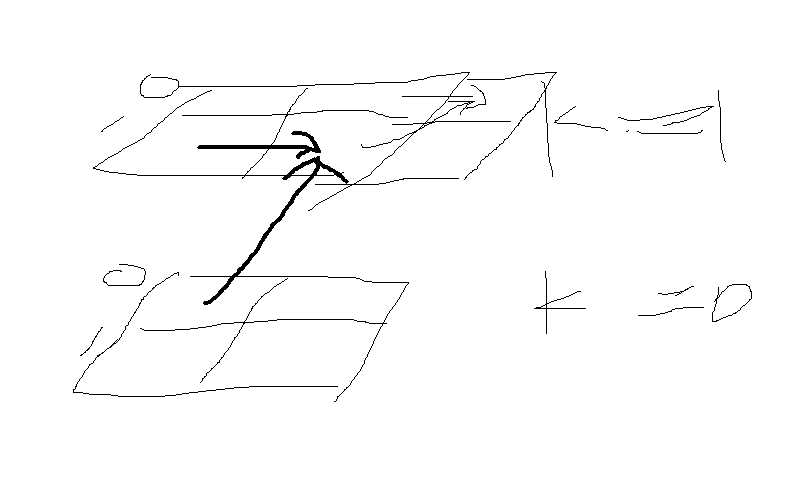
\includegraphics[width=0.7\linewidth]{pics/stock.png}
		
	\item 三个问题: matrix 和气球问题, 二维数组,答案在右上角, 需要使用倾斜遍历或者反向遍历。转换方程也几乎一致。
	
\begin{lstlisting}
	for (int i = n; i >= 0; i--) {
		// j 应该从左往右
		for (int j = i + 1; j < n + 2; j++) {
			// 最后戳破的气球是哪个?
			for (int k = i + 1; k < j; k++) {
				// 择优做选择
				dp[i][j] = Math.max(
				dp[i][j], 
				dp[i][k] + dp[k][j] + points[i]*points[j]*points[k]
				);
			}
		}
	}
\end{lstlisting}
另外一个问题是正则表达式和编辑距离, 结果在右下角, 正向遍历。 子函数代表一种编辑或匹配动作。
\begin{lstlisting}
bool dp(string& s, int i, string& p, int j) {
	if (s[i] == p[j] || p[j] == '.') {
		// 匹配
		if (j < p.size() - 1 && p[j + 1] == '*') {
			// 1.1 通配符匹配 0 次或多次
			return dp(s, i, p, j + 2)
			|| dp(s, i + 1, p, j);
		} else {
			// 1.2 常规匹配 1 次
			return dp(s, i + 1, p, j + 1);
		}
	} else {
		// 不匹配
		if (j < p.size() - 1 && p[j + 1] == '*') {
			// 2.1 通配符匹配 0 次
			return dp(s, i, p, j + 2);
		} else {
			// 2.2 无法继续匹配
			return false;
		}
	}
}

// 定义:返回 s1[0..i] 和 s2[0..j] 的最小编辑距离
int dp(String s1, int i, String s2, int j) {
	// base case
	if (i == -1) return j + 1;
	if (j == -1) return i + 1;
	
	if (s1.charAt(i) == s2.charAt(j)) {
		return dp(s1, i - 1, s2, j - 1); // 啥都不做
	}
	return min(
	dp(s1, i, s2, j - 1) + 1,    // 插入
	dp(s1, i - 1, s2, j) + 1,    // 删除
	dp(s1, i - 1, s2, j - 1) + 1 // 替换
	);
}

\end{lstlisting}
另外一个问题就是鸡蛋和最小子集和, 答案在右下角, 需要利用k遍历前面所有的, 然后所有最大的可能中,区一个最小的。 (至少需要。。。)
子集分割是, 思路就是鸡蛋的思路, 
\begin{lstlisting}
	
	for (int i = 1; i <= n; ++i) {
		for (int j = 1; j <= min(i, m); ++j) {
			if (j == 1) {
				dp[i][j] = sum[i];
			} else {
				for (int k = 1; k <= i - 1; ++k) {
					dp[i][j] = min(dp[i][j], max(dp[k][j - 1], sum[i] - sum[k]));
				}
			}
		}
	}
\end{lstlisting}

另外一个问题就是背包和换零钱二, 答案在右下角,选择是有限的几个(物品或者钱)。

面试的时候优先用top down, 递归方式。 关键是遍历所有选项,根据选项改变状态后, 把新状态传入子问题。 然后在对结果进行处理,有点后序遍历的味道。 这一点很重要。
\begin{lstlisting}
int knapSack(int W, int wt[], int val[], int n)
{
	
	// Base Case
	if (n == 0 || W == 0)
	return 0;
	
	// If weight of the nth item is more
	// than Knapsack capacity W, then
	// this item cannot be included
	// in the optimal solution
	if (wt[n - 1] > W)
	return knapSack(W, wt, val, n - 1);
	
	// Return the maximum of two cases:
	// (1) nth item included
	// (2) not included
	else
	//选项有两个,所以不用写for了, 根据选项改变了状态,然后把状态传入递归调用,返回的结果进行max. 
	return max(
	val[n - 1]
	+ knapSack(W - wt[n - 1], 
	wt, val, n - 1),
	knapSack(W, wt, val, n - 1));
}	
\end{lstlisting}

另外一个问题就是 lcs, 编辑距离和最长回文子序列。 不同的状态转移, 遍历方向和初始条件, 具体的细节可以参考前面dp一章。 


		
\end{itemize}

\section{backtrace}
\begin{itemize}
	\item 形式一、元素无重不可复选,即 nums 中的元素都是唯一的,每个元素最多只能被使用一次,这也是最基本的形式。
	
	以组合为例,如果输入 nums = [2,3,6,7],和为 7 的组合应该只有 [7]。
	
	形式二、元素可重不可复选,即 nums 中的元素可以存在重复,每个元素最多只能被使用一次。
	
	以组合为例,如果输入 nums = [2,5,2,1,2],和为 7 的组合应该有两种 [2,2,2,1] 和 [5,2]。
	
	形式三、元素无重可复选,即 nums 中的元素都是唯一的,每个元素可以被使用若干次。
	
	以组合为例,如果输入 nums = [2,3,6,7],和为 7 的组合应该有两种 [2,2,3] 和 [7]。
	
	当然,也可以说有第四种形式,即元素可重可复选。但既然元素可复选,那又何必存在重复元素呢?元素去重之后就等同于形式三,所以这种情况不用考虑。
	上面用组合问题举的例子,但排列、组合、子集问题都可以有这三种基本形式,所以共有 9 种变化。
	
	\item 1) use ,我们使用 start 参数控制树枝的生长避免产生重复的子集,用 track 记录根节点到每个节点的路径的值,同时在前序位置把每个节点的路径值收集起来,完成回溯树的遍历就收集了所有子集:
	
	\begin{lstlisting}
		List<List<Integer>> res = new LinkedList<>();
		// 记录回溯算法的递归路径
		LinkedList<Integer> track = new LinkedList<>();
		
		// 主函数
		public List<List<Integer>> subsets(int[] nums) {
			backtrack(nums, 0);
			return res;
		}
		
		// 回溯算法核心函数,遍历子集问题的回溯树
		void backtrack(int[] nums, int start) {
			
			// 前序位置,每个节点的值都是一个子集
			res.add(new LinkedList<>(track));
			
			// 回溯算法标准框架
			for (int i = start; i < nums.length; i++) {
				// 做选择
				track.addLast(nums[i]);
				// 通过 start 参数控制树枝的遍历,避免产生重复的子集
				backtrack(nums, i + 1);
				// 撤销选择
				track.removeLast();
			}
		}
	\end{lstlisting}
	
	2) 现在你只需要把第 2 层(根节点视为第 0 层)的节点收集起来,就是大小为 2 的所有组合:
	
	3) 排列,  没有start, 用used
	
	\begin{lstlisting}
		List<List<Integer>> res = new LinkedList<>();
		// 记录回溯算法的递归路径
		LinkedList<Integer> track = new LinkedList<>();
		// track 中的元素会被标记为 true
		boolean[] used;
		
		/* 主函数,输入一组不重复的数字,返回它们的全排列 */
		public List<List<Integer>> permute(int[] nums) {
			used = new boolean[nums.length];
			backtrack(nums);
			return res;
		}
		
		// 回溯算法核心函数
		void backtrack(int[] nums) {
			// base case,到达叶子节点
			if (track.size() == nums.length) {
				// 收集叶子节点上的值
				res.add(new LinkedList(track));
				return;
			}
			
			// 回溯算法标准框架
			for (int i = 0; i < nums.length; i++) {
				// 已经存在 track 中的元素,不能重复选择
				if (used[i]) {
					continue;
				}
				// 做选择
				used[i] = true;
				track.addLast(nums[i]);
				// 进入下一层回溯树
				backtrack(nums);
				// 取消选择
				track.removeLast();
				used[i] = false;
			}
		}
	\end{lstlisting}
	
	4) 体现在代码上,需要先进行排序,让相同的元素靠在一起,如果发现 nums[i] == nums[i-1],则跳过:
	5) 同 2
	6)  if (i > 0 && nums[i] == nums[i - 1] && !used[i - 1]) {
		// 如果前面的相邻相等元素没有用过,则跳过
		continue;
	}
	
	7)// 可重组合的回溯算法框架
	void backtrack(int[] nums, int start) {
		for (int i = start; i < nums.length; i++) {
			// ...
			// 递归遍历下一层回溯树,注意参数
			backtrack(nums, i);
			// ...
		}
	} 这样这棵回溯树会永远生长下去,所以我们的递归函数需要设置合适的 base case 以结束算法,即路径和大于 target 时就没必要再遍历下去了。
	
	8) 同5
	9) 不用used. 
	
	\item 
	\begin{lstlisting}
		// 二叉树遍历框架
		void traverse(TreeNode root) {
			traverse(root.left);
			traverse(root.right);
		}
		
		// 二维矩阵遍历框架
		void dfs(int[][] grid, int i, int j, boolean[][] visited) {
			int m = grid.length, n = grid[0].length;
			if (i < 0 || j < 0 || i >= m || j >= n) {
				// 超出索引边界
				return;
			}
			if (visited[i][j]) {
				// 已遍历过 (i, j)
				return;
			}
			// 进入节点 (i, j)
			visited[i][j] = true;
			dfs(grid, i - 1, j, visited); // 上
			dfs(grid, i + 1, j, visited); // 下
			dfs(grid, i, j - 1, visited); // 左
			dfs(grid, i, j + 1, visited); // 右
		}
	\end{lstlisting}

	\item 所有自己, 就有两种观点,一个是球, 一个是桶。 会有两种形状的树, 但是结果一样。  桶观点是偏多叉树。 可以这么理解。 分为有1和没有1, 在没有1里面再分有2没有2.  1, 2, 3, 4都没有, 就单独选5.  
	
	\item 利用桶的观点, 可以解决分割K个等和的子集. 1) 注意k, 这个可以类比与股票买卖中的交易次数, 可以把他用在(动态, 回溯中) , 满足了target, 就把k-1. 2) 第二个思想就是用桶的观点去回溯生成组合子集。 3) 第三个观点是return false用于剪枝
	这是一个很有代表性的题目, 貌似不能用dp求解, 只能
\begin{lstlisting}
class Solution {
	public:
	bool canPartitionKSubsets(vector<int>& nums, int k) {
		int sum = accumulate(nums.begin(), nums.end(), 0);
		if (sum % k != 0) return false;
		sort(nums.begin(), nums.end(), greater<int>());
		vector<bool> visited(nums.size(), false);
		return helper(nums, k, sum / k, 0, 0, visited);
	}
	bool helper(vector<int>& nums, int k, int target, int start, int curSum, vector<bool>& visited) {
		if (k == 1) return true;
		if (curSum > target) return false; //第三个观点是return false用于剪枝
		if (curSum == target) return helper(nums, k - 1, target, 0, 0, visited);  
		for (int i = start; i < nums.size(); ++i) {
			if (visited[i]) continue;
			visited[i] = true;
			if (helper(nums, k, target, i + 1, curSum + nums[i], visited)) return true;
			visited[i] = false;
		}
		return false;
	}
};
\end{lstlisting}
	
	
\end{itemize}

\section{tree}
\begin{itemize}
	\item 只要是递归, 一定要有base case, 如果函数有值, 一定要用return.  很重要
	
	\item 滑动窗口,模板代码
	
	\item  while 模式程序
	\begin{lstlisting}
		init flag;
		while(flag != ***){
			...
			update flag
		}
	\end{lstlisting}

	\item 有的树需要输入两个节点。
	
	\item 如果可以用全局变量,最好用全局变量, 然后把递归函数的返回值定位 void, 这样可以避免很多return 和复杂的逻辑。 两个例子就是leetcode 的 left leaves sum 和 word search.
	
\item 1、是否可以通过遍历一遍二叉树得到答案?如果可以,用一个 traverse 函数配合外部变量来实现,这叫「遍历」的思维模式。

2、是否可以定义一个递归函数,通过子问题(子树)的答案推导出原问题的答案?如果可以,写出这个递归函数的定义,并充分利用这个函数的返回值,这叫「分解问题」的思维模式。

无论使用哪种思维模式,你都需要思考:

3、如果单独抽出一个二叉树节点,它需要做什么事情?需要在什么时候(前/中/后序位置)做?其他的节点不用你操心,递归函数会帮你在所有节点上执行相同的操作。

\item 全局变量, 引用变量, 局部变量, 返回变量, 四个变量用在树递归程序中的区别。

\item 讲到这里,照应一下前文:遇到子树问题,首先想到的是给函数设置返回值,然后在后序位置做文章。

反过来,如果你写出了类似一开始的那种递归套递归的解法,大概率也需要反思是不是可以通过后序遍历优化了。

\begin{lstlisting}
	// 遍历二叉树
	void traverse(TreeNode root) {
		if (root == null) {
			return;
		}
		// 对每个节点计算直径
		int leftMax = maxDepth(root.left);  //递归套递归
		int rightMax = maxDepth(root.right);
		int myDiameter = leftMax + rightMax;
		// 更新全局最大直径
		maxDiameter = Math.max(maxDiameter, myDiameter);
		
		traverse(root.left);
		traverse(root.right);
	}
\end{lstlisting}

\item 二叉树的构造问题一般都是使用「分解问题」的思路:构造整棵树 = 根节点 + 构造左子树 + 构造右子树。

\item 返回节点的有两道题, 一个是公共祖先,一个是删除BST的某个值的节点。

\item 	二叉树题目的递归解法可以分两类思路,第一类是遍历一遍二叉树得出答案,第二类是通过分解问题计算出答案,这两类思路分别对应着 回溯算法核心框架 和 动态规划核心框架。


\item  中序位置主要用在 BST 场景中,你完全可以把 BST 的中序遍历认为是遍历有序数组。

前序位置本身其实没有什么特别的性质,之所以你发现好像很多题都是在前序位置写代码,实际上是因为我们习惯把那些对前中后序位置不敏感的代码写在前序位置罢了。

你可以发现,前序位置的代码执行是自顶向下的,而后序位置的代码执行是自底向上的: 但这里面大有玄妙,意味着前序位置的代码只能从函数参数中获取父节点传递来的数据,而后序位置的代码不仅可以获取参数数据,还可以获取到子树通过函数返回值传递回来的数据。

	
\end{itemize}

\section{dc}
\begin{itemize}
	\item 二分思想一个应用是板子上点最近距离, 可以利用一个子问题来剪掉一些候选点。另外一个应用是利用归并排序计算右侧小的元素, labuladon 有介绍。根本思想还是二分, 具体上是因为归并排序有序性, 所以可以利用这个特点计算右侧小于的元素。 比较有特点。	
\end{itemize}

\begin{itemize}

\section{other}
\begin{itemize}
	\item 	数据结构的存储方式只有两种:数组(顺序存储)和链表(链式存储)。 数据结构种类很多,但它们存在的目的都是在不同的应用场景,尽可能高效地增删查改。
	
	\item 	我的建议是直接在递归函数内部打印关键值,配合缩进,直观地观察递归函数执行情况。
	
	\item 位操作: 四个基本操作,两个移动。 如何set, clear, toggle, check 某个位? 如何clear 最左,最右位? 
	
	\begin{lstlisting}
		int msb = 0;
		n = n / 2;
		while (n != 0) {
			n = n / 2;
			msb++;
		}
	\end{lstlisting}

\item slow, fast代码 实现的remove 和unique.  不等于就copy, 然后slow加1. partition 也是这个思路, 只不过是不能copy, 而是switch. 
	\begin{lstlisting}
int removeDuplicates(int[] nums) {
	if (nums.length == 0) {
		return 0;
	}
	int slow = 0, fast = 0;
	while (fast < nums.length) {
		if (nums[fast] != nums[slow]) {
			slow++;
			// 维护 nums[0..slow] 无重复
			nums[slow] = nums[fast];
		}
		fast++;
	}
	// 数组长度为索引 + 1
	return slow + 1;
}
	\end{lstlisting}

	\begin{lstlisting}
	int removeElement(int[] nums, int val) {
		int fast = 0, slow = 0;
		while (fast < nums.length) {
			if (nums[fast] != val) {
				nums[slow] = nums[fast];
				slow++;
			}
			fast++;
		}
		return slow;
	}
\end{lstlisting}

\end{itemize}
	

\section{greed}
\begin{itemize}

\item 时间调度7个题: 1)至少需要几个会议室? 启点排序,然后用结束时间放于最小堆最小堆。 2)一个会议室最多安排几个会议? 会议终点排序,然后用终点删掉相交的线段(唯一一个终点排序

)3) 删掉覆盖区间, 起点升序排列,终点降序排列。 只维护left and right.
\begin{lstlisting}
if (left <= intv[0] && right >= intv[1]) {
	res++;
}
// 情况二,找到相交区间,合并
if (right >= intv[0] && right <= intv[1]) {
	right = intv[1];
}
// 情况三,完全不相交,更新起点和终点
if (right < intv[0]) {
	left = intv[0];
	right = intv[1];
}
\end{lstlisting}
4) 合并区间, 和删除覆盖区间的原理一样。
\begin{lstlisting}
res.append(intervals[0])

for i in range(1, len(intervals)):
	curr = intervals[i]
	# res 中最后一个元素的引用
	last = res[-1]
	if curr[0] <= last[1]:
		# 找到最大的 end
		last[1] = max(last[1], curr[1])
	else:
		# 处理下一个待合并区间
		res.append(curr)
return res
\end{lstlisting}

5) 最小视频 我们会比较所有起点小于clips[0][1]的区间,根据贪心策略,它们中终点最大的那个区间就是第二个会被选中的视频。

然后可以通过第二个视频区间贪心选择出第三个视频,以此类推,直到覆盖区间[0, T],或者无法覆盖返回 -1。

6) 两个区间队列交集。
\begin{lstlisting}
while i < len(A) and j < len(B):
a1, a2 = A[i][0], A[i][1]
b1, b2 = B[j][0], B[j][1]
# 两个区间存在交集
if b2 >= a1 and a2 >= b1:
	# 计算出交集,加入 res
	res.append([max(a1, b1), min(a2, b2)])
	# 指针前进
	if b2 < a2: j += 1
	else:       i += 1
\end{lstlisting}

\end{itemize}
	
\section{template code}
	\item 
\begin{lstlisting}
	/* 滑动窗口算法框架 */
	void slidingWindow(string s, string t) {
		unordered_map<char, int> need, window;
		for (char c : t) need[c]++;
		
		int left = 0, right = 0;
		int valid = 0; 
		while (right < s.size()) {
			// c 是将移入窗口的字符
			char c = s[right];
			// 增大窗口
			right++;
			// 进行窗口内数据的一系列更新
			...
			
			/*** debug 输出的位置 ***/
			printf("window: [%d, %d)\n", left, right);
			/********************/
			
			// 判断左侧窗口是否要收缩
			while (window needs shrink) {
				// d 是将移出窗口的字符
				char d = s[left];
				// 缩小窗口
				left++;
				// 进行窗口内数据的一系列更新
				...
			}
		}
	}
\end{lstlisting}
	
	\item BFS, DFS template code
	\item dp, inorder, reverse order and diaginal traverse
	
	\item why palindrome and matrix need two dimension array. 
\begin{lstlisting}
for(int l = 2; l<n ; l++)
	for(int i = 0; i<n -1;i++)
	   int j = 1+i-1 ...
\end{lstlisting}
	
	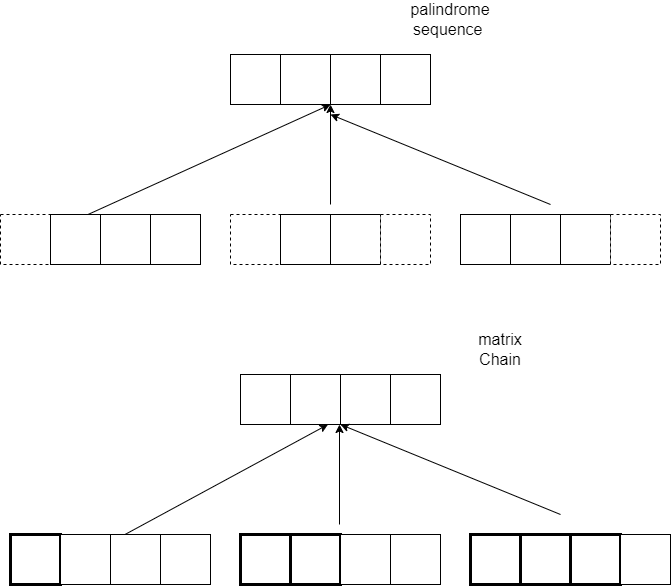
\includegraphics[scale=0.25]{pics/dp.drawio.png}
	
	\item back trace template code
	\item binary search 
	\item tree's recursion idea
	\item 移动窗口代码。
	
	\item merge
\begin{lstlisting}
 // 用于辅助合并有序数组
private static int[] temp;

public static void sort(int[] nums) {
	// 先给辅助数组开辟内存空间
	temp = new int[nums.length];
	// 排序整个数组(原地修改)
	sort(nums, 0, nums.length - 1);
}

// 定义:将子数组 nums[lo..hi] 进行排序
private static void sort(int[] nums, int lo, int hi) {
	if (lo == hi) {
		// 单个元素不用排序
		return;
	}
	// 这样写是为了防止溢出,效果等同于 (hi + lo) / 2
	int mid = lo + (hi - lo) / 2;
	// 先对左半部分数组 nums[lo..mid] 排序
	sort(nums, lo, mid);
	// 再对右半部分数组 nums[mid+1..hi] 排序
	sort(nums, mid + 1, hi);
	// 将两部分有序数组合并成一个有序数组
	merge(nums, lo, mid, hi);
}

// 将 nums[lo..mid] 和 nums[mid+1..hi] 这两个有序数组合并成一个有序数组
private static void merge(int[] nums, int lo, int mid, int hi) {
	// 先把 nums[lo..hi] 复制到辅助数组中
	// 以便合并后的结果能够直接存入 nums
	for (int i = lo; i <= hi; i++) {
		temp[i] = nums[i];
	}
	
	// 数组双指针技巧,合并两个有序数组
	int i = lo, j = mid + 1;
	for (int p = lo; p <= hi; p++) {
		if (i == mid + 1) {
			// 左半边数组已全部被合并
			nums[p] = temp[j++];
		} else if (j == hi + 1) {
			// 右半边数组已全部被合并
			nums[p] = temp[i++];
		} else if (temp[i] > temp[j]) {
			nums[p] = temp[j++];
		} else {
			nums[p] = temp[i++];
		}
	}
}
}
\end{lstlisting}

	\item uf code, use recursive find is very tricky :)
\begin{lstlisting}
	class UF {
		// 连通分量个数
		private int count;
		// 存储每个节点的父节点
		private int[] parent;
		
		// n 为图中节点的个数
		public UF(int n) {
			this.count = n;
			parent = new int[n];
			for (int i = 0; i < n; i++) {
				parent[i] = i;
			}
		}
		
		// 将节点 p 和节点 q 连通
		public void union(int p, int q) {
			int rootP = find(p);
			int rootQ = find(q);
			
			if (rootP == rootQ)
			return;
			
			parent[rootQ] = rootP;
			// 两个连通分量合并成一个连通分量
			count--;
		}
		
		// 判断节点 p 和节点 q 是否连通
		public boolean connected(int p, int q) {
			int rootP = find(p);
			int rootQ = find(q);
			return rootP == rootQ;
		}
		
		public int find(int x) {
			if (parent[x] != x) {
				parent[x] = find(parent[x]);
			}
			return parent[x];
		}
		
		// 返回图中的连通分量个数
		public int count() {
			return count;
		}
	}
\end{lstlisting}


	\item 二维数组的初始化, 二维数组用于背包, 还有动态规划问题。 矩阵和. base case都是零。

\begin{lstlisting}
	vector<vector<int> > matrix;
	matrix.resize(m);
	for(auto &e : matrix)
		e.resize(n, 0);
\end{lstlisting}

	\item 数据结构设计, 1) hash list 2) FV 频率值 -> hash  hash list 用于LRU LFU. 
	
	\item 括号问题, 1) 合法性(数数) + 栈, 2) 生成(回溯)
	
	\item 链表中dummy node的使用
	
	\item 二维数组遍历。 岛屿问题。
\begin{lstlisting}
	// 从 (i, j) 开始,将与之相邻的陆地都变成海⽔
	void dfs(char[][] grid, int i, int j) {
		int m = grid.length, n = grid[0].length;
		if (i < 0 || j < 0 || i >= m || j >= n) {
			// 超出索引边界
			return;
		}
		if (grid[i][j] == '0') {
			// 已经是海⽔了
			return;
		}
		// 将 (i, j) 变成海⽔
		grid[i][j] = '0';
		// 淹没上下左右的陆地
		dfs(grid, i + 1, j);
		dfs(grid, i, j + 1);
		dfs(grid, i - 1, j);
		dfs(grid, i, j - 1);
	}
}
\end{lstlisting}

\item 我们一般是通过 \% 运算符求模(余数),来模拟环形特效:
\begin{lstlisting}
int[] arr = {1,2,3,4,5};
int n = arr.length, index = 0;
while (true) {
	// 在环形数组中转圈
	print(arr[index % n]);
	index++;
}

int[] nextGreaterElements(int[] nums) {
	int n = nums.length;
	int[] res = new int[n];
	Stack<Integer> s = new Stack<>();
	// 数组长度加倍模拟环形数组
	for (int i = 2 * n - 1; i >= 0; i--) {
		// 索引 i 要求模,其他的和模板一样
		while (!s.isEmpty() && s.peek() <= nums[i % n]) {
		s.pop();
	}
	res[i % n] = s.isEmpty() ? -1 : s.peek();
	s.push(nums[i % n]);
}
return res;
}
\end{lstlisting}

\item C++ does not offer a collection template with the behavior that would mimic Java's LinkedHashMap<K,V>, so you would need to maintain the order separately from the mapping.

This can be achieved by keeping the data in a std::list<std::pair<K,V>>, and keeping a separate std::unordered_map<k,std::list<std::pair<K,V>>::iterator> map for quick look-up of the item by key:

\begin{enumerate}
	\item On adding an item, add the corresponding key/value pair to the end of the list, and map the key to the iterator std::prev(list.end()).
	
	\item On removing an item by key, look up its iterator, remove it from the list, and then remove the mapping.
	
	\item On replacing an item, look up list iterator from the unordered map first, and then replace its content with a new key-value pair.
	
	\item On iterating the values, simply iterate std::list<std::pair<K,V>>.
\end{enumerate}

	
\end{itemize}

\section{project}
\begin{itemize}
	\item drop of knowledge C++, sixth edition. includes all modern C++ 17/20 features. This year, I will add test and internet two chapters.  Such as move semantic,  smart pointer, concurrency, brace initialization and generic programming. 
	
	\item A compiler project. Intermediate representation, Whirl to LLVM. 
	
	\item A Trade Repository or Swap Data Repository is an entity that centrally collects and maintains the records of over-the-counter (OTC) derivatives. CFTC. Commodity Futures Trading Commission.   Athena is a cross-asset platform transforming technology at JP Morgan. It delivers innovative and efficient applications to a wide range of the firm's businesses, including sales, trading, operations, risk and research. Athena combined the best of open source technologies
	
	\item There are two main types of RFID tags: battery-operated and passive. 
	
\fi

\end{itemize}


\ifx \allfiles \undefined
%\end{CJK*}
\end{document}
\fi
